%% Generated by Sphinx.
\def\sphinxdocclass{report}
\documentclass[a4paper,11pt,english,openany,oneside]{sphinxmanual}
\ifdefined\pdfpxdimen
   \let\sphinxpxdimen\pdfpxdimen\else\newdimen\sphinxpxdimen
\fi \sphinxpxdimen=.75bp\relax
\ifdefined\pdfimageresolution
    \pdfimageresolution= \numexpr \dimexpr1in\relax/\sphinxpxdimen\relax
\fi
\newdimen\sphinxremdimen\sphinxremdimen = 11pt
%% let collapsible pdf bookmarks panel have high depth per default
\PassOptionsToPackage{bookmarksdepth=5}{hyperref}

\PassOptionsToPackage{booktabs}{sphinx}

\PassOptionsToPackage{warn}{textcomp}


\usepackage{cmap}
\usepackage{xeCJK}
\usepackage{amsmath,amssymb,amstext}
\usepackage{babel}



\setmainfont{FreeSerif}[
  Extension      = .otf,
  UprightFont    = *,
  ItalicFont     = *Italic,
  BoldFont       = *Bold,
  BoldItalicFont = *BoldItalic
]
\setsansfont{FreeSans}[
  Extension      = .otf,
  UprightFont    = *,
  ItalicFont     = *Oblique,
  BoldFont       = *Bold,
  BoldItalicFont = *BoldOblique,
]
\setmonofont{FreeMono}[Scale=0.9,
  Extension      = .otf,
  UprightFont    = *,
  ItalicFont     = *Oblique,
  BoldFont       = *Bold,
  BoldItalicFont = *BoldOblique,
]



\usepackage[Sonny]{fncychap}
\usepackage[,numfigreset=1,mathnumfig,mathnumsep={.}]{sphinx}

\fvset{fontsize=\small,formatcom=\xeCJKVerbAddon}
\usepackage{geometry}


% Include hyperref last.
\usepackage{hyperref}
% Fix anchor placement for figures with captions.
\usepackage{hypcap}% it must be loaded after hyperref.
% Set up styles of URL: it should be placed after hyperref.
\urlstyle{same}

\addto\captionsenglish{\renewcommand{\contentsname}{目录}}

\usepackage{sphinxmessages}
\setcounter{tocdepth}{3}
\setcounter{secnumdepth}{3}


% ===== 中文支持 =====
\usepackage{xeCJK}
\usepackage[fontset=windows]{ctex}

% ===== 页面边距与页眉空间分配 =====
\usepackage{geometry}
\geometry{
    left=25mm,
    right=25mm,
    top=30mm,
    bottom=25mm,
    headheight=25pt, % 留足页眉高度
    headsep=8mm      % 页眉与正文的距离
}

% ===== 图片路径 =====
\graphicspath{{images/}}

% ===== 禁止图表浮动 =====
\usepackage{float}
\usepackage{placeins}

\makeatletter
\def\fps@figure{H}
\def\fps@table{H}
\def\fps@sphinxfigure{H}
\def\fps@sphinxTable{H}
\makeatother

% ==== 强制图片后换行 ===
\usepackage{etoolbox}
\AtEndEnvironment{figure}{\par\noindent}
\AtEndEnvironment{sphinxfigure}{\par\noindent}

% ===== 代码高亮 =====
\usepackage{listings}

% ===== PDF书签 =====
\usepackage{bookmark}

% ===== 自定义变量 =====
\newcommand{\docversion}{V01}
\newcommand{\docname}{iM-D硬件用户手册}

% ===== 页眉页脚 (恢复 LastPage 避免??) =====
\usepackage{fancyhdr}
\usepackage{lastpage} 

% 1. 重定义 Sphinx 的正文页样式 (normal)
\fancypagestyle{normal}{
    \fancyhf{}  
    \fancyhead[L]{\raisebox{-0.15cm}{
\includegraphics[height=0.7cm]{Logo.png}}}
    \fancyhead[R]{\nouppercase{\leftmark}}  
    \fancyfoot[L]{版本 \docversion}
    % 使用最稳定的 LastPage
    \fancyfoot[C]{\thepage/\pageref*{LastPage}}
    \fancyfoot[R]{\docname}
    \renewcommand{\headrulewidth}{0.4pt} 
    \renewcommand{\footrulewidth}{0.4pt}
}

% 2. 重定义 Sphinx 的章节起始页样式 (plain)
\fancypagestyle{plain}{
    \fancyhf{}
    \fancyhead[L]{\raisebox{-0.15cm}{
\includegraphics[height=0.7cm]{Logo.png}}}
    \fancyfoot[L]{版本 \docversion}
    \fancyfoot[C]{\thepage/\pageref*{LastPage}}
    \fancyfoot[R]{\docname}
    \renewcommand{\headrulewidth}{0pt}   
    \renewcommand{\footrulewidth}{0.4pt}
}

% ===== 标题样式 =====
\usepackage{titlesec}
\usepackage{xcolor}

% 定义红色
\definecolor{TitleRed}{HTML}{D80C1E}

% 章节间距
\titlespacing*{\chapter}{0pt}{-30pt}{20pt}

% Chapter
\titleformat{\chapter}
{\Huge\bfseries\color{TitleRed}}
{\thechapter}{0.5em}{}

% Section
\titleformat{\section}
{\Large\bfseries\color{TitleRed}}
{\thesection}{0.5em}{}

% Subsection
\titleformat{\subsection}
{\large\bfseries\color{TitleRed}}
{\thesubsection}{0.5em}{}

% Subsubsection
\titleformat{\subsubsection}
{\normalsize\bfseries\color{TitleRed}}
{\thesubsubsection}{0.5em}{}

% ===== 超链接颜色 =====
\usepackage{hyperref}

\hypersetup{
colorlinks=true,
linkcolor=blue,
urlcolor=blue,
citecolor=blue
}

% ===== 所有目录页变黑，正文恢复蓝色 (强力黑盒覆盖版) =====

% 1. 主目录
\let\origsphinxtableofcontents\sphinxtableofcontents
\renewcommand{\sphinxtableofcontents}{
    \begingroup
    \cleardoublepage
    \pagenumbering{Roman}
    \pagestyle{plain} 
    \hypersetup{linkcolor=black}
    \origsphinxtableofcontents
    \clearpage
    \endgroup
    \pagenumbering{arabic}
    \pagestyle{normal}
}

% 2. 图目录
\let\origlistoffigures\listoffigures
\renewcommand{\listoffigures}{
    \begingroup
    \hypersetup{linkcolor=black}
    \origlistoffigures
    \endgroup
}

% 3. 表目录
\let\origlistoftables\listoftables
\renewcommand{\listoftables}{
    \begingroup
    \hypersetup{linkcolor=black}
    \origlistoftables
    \endgroup
}

% ===== 表格样式 =====
\usepackage{colortbl}
\usepackage{longtable}
\usepackage{booktabs}

\definecolor{tableheader}{RGB}{200,0,0}
\definecolor{tableborder}{RGB}{160,160,160}

\arrayrulecolor{tableborder}

% 表头样式
\renewcommand{\sphinxstyletheadfamily}{
\color{white}\bfseries
}

\newcommand{\sphinxstyletheadbackground}{
\rowcolor{tableheader}
}

\appto\sphinxstyletheadfamily{\sphinxstyletheadbackground}

% ===== 表格跨页与宽度控制 =====
\usepackage{tabularx}
\usepackage{ltablex}
\keepXColumns

% 表格自动换行
\renewcommand{\tabularxcolumn}[1]{m{#1}}

% 表格不要超出页边距
\setlength{\LTleft}{0pt}
\setlength{\LTright}{0pt}

% ===== 代码块分页优化 =====
\sphinxsetup{
verbatimwithframe=false
}

\usepackage{tocloft}

% ===== 中文图表名称 =====
\AtBeginDocument{
    \renewcommand{\figurename}{图}
    \renewcommand{\tablename}{表}
    \renewcommand{\listfigurename}{图目录}
    \renewcommand{\listtablename}{表目录}
    
    % 防止图表目录编号和名称重叠
    \setlength{\cftfignumwidth}{3em}
    \setlength{\cfttabnumwidth}{3em}
}



\title{iM-D硬件用户手册}
\date{2026 年 03 月 30 日}
\release{V01}
\author{JAKA}
\newcommand{\sphinxlogo}{\vbox{}}
\renewcommand{\releasename}{版本}
\makeindex
\begin{document}

\ifdefined\shorthandoff
  \ifnum\catcode`\=\string=\active\shorthandoff{=}\fi
  \ifnum\catcode`\"=\active\shorthandoff{"}\fi
\fi

\pagestyle{empty}
\begin{titlepage}
    \thispagestyle{empty}
    \centering

\vspace*{1cm}

    % 顶部 JAKA 图片
    
\includegraphics[width=0.4\textwidth]{Logo.png} \\[1cm]

    % 硬件用户手册
    {\huge 硬件用户手册\par}
    \vspace{1cm}

    % 产品图
    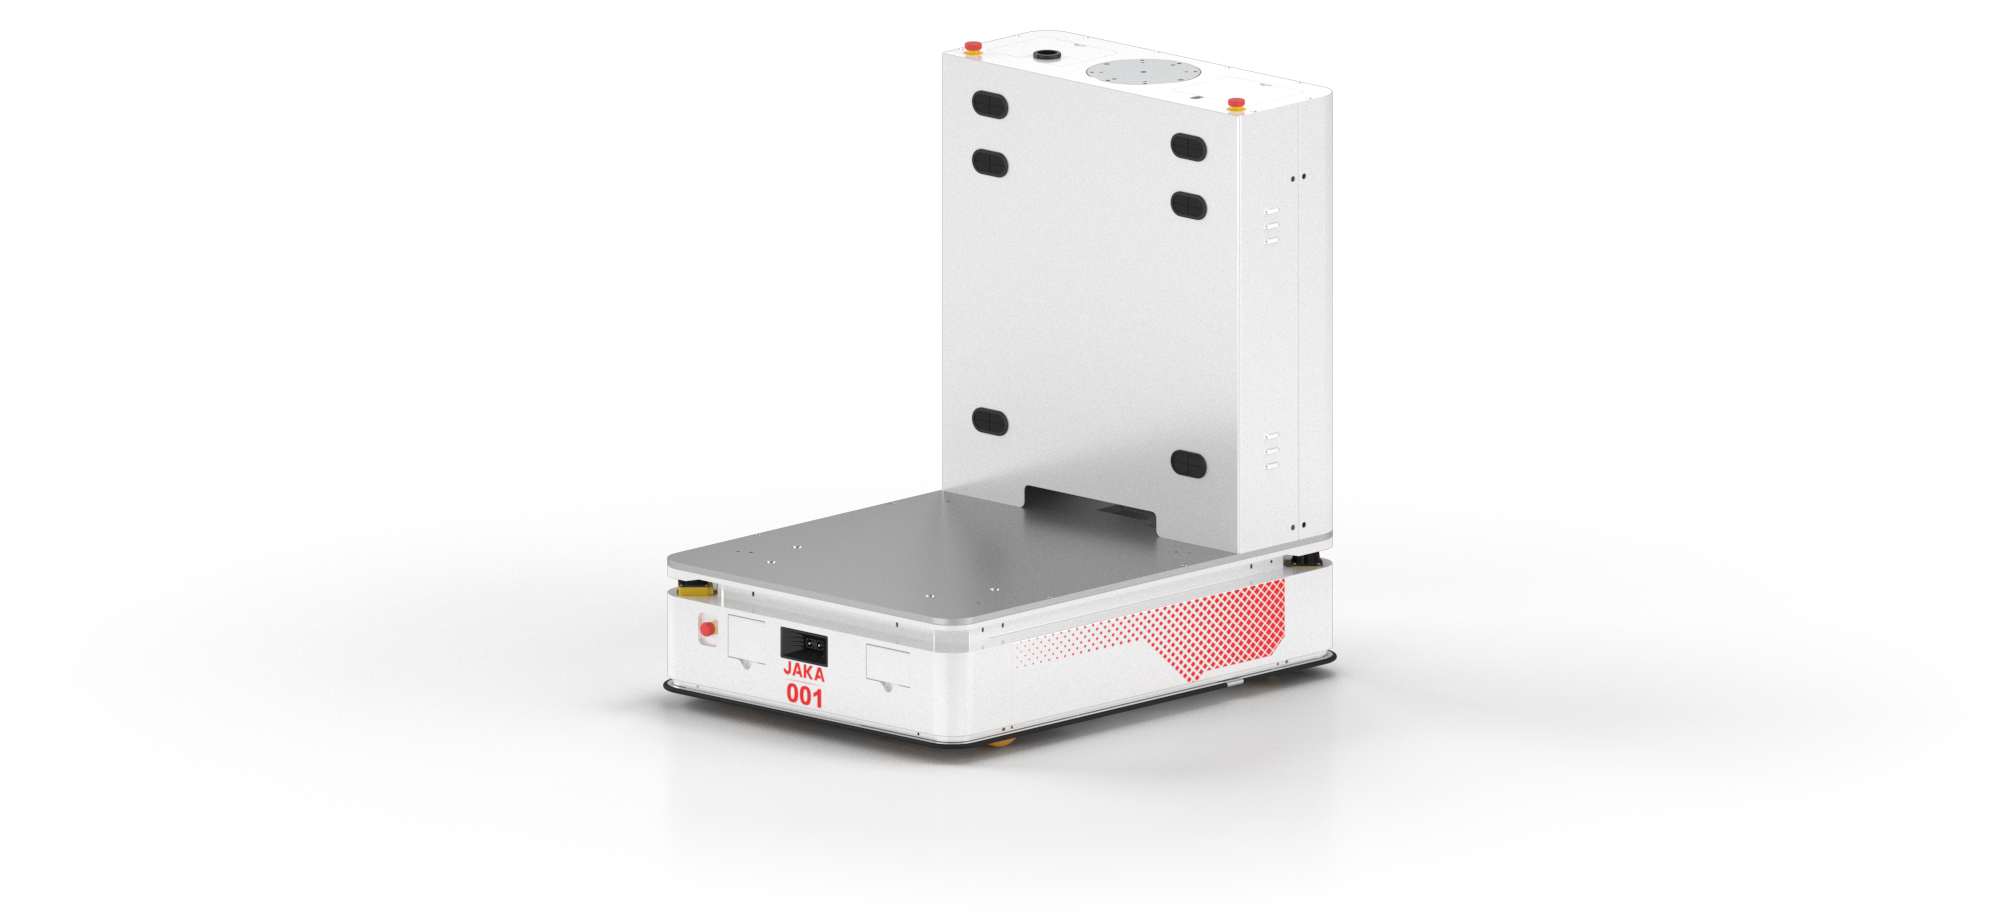
\includegraphics[width=1.0\textwidth]{iM-D.png} \\[1cm]
    
    % 型号名称
    {\LARGE JAKA iM-D\par}
    \vspace{0.5cm}
    
    % 版本信息
    {\large 翻译版本（zh）\par}
    {\large 文档版本：\docversion\par}

    \vspace{\fill}
    
    % 底部信息（右对齐）
    \begin{flushright}
        \large
        机器人：Zu，Pro，S，A系列 \\
        控制柜：RoboHub \\
        软件：V3.3.8及以上版本Coboπ App \\
    \end{flushright}
    
    \vspace{1cm}
\end{titlepage}
\pagestyle{plain}
\sphinxtableofcontents
\pagestyle{normal}
\phantomsection\label{\detokenize{index::doc}}


\sphinxAtStartPar
本手册是节卡机器人股份有限公司（后文统称为“节卡”或“JAKA”）的专有财产，其版权及解释权归JAKA及其关联公司所有。未经JAKA的书面同意，其他任何方不得以任何形式使用其内容。

\sphinxAtStartPar
JAKA会定期对手册进行修正和完善，其内容可能会更新，恕不另行通知。使用本手册前请认真核对实际产品信息。

\sphinxAtStartPar
本手册适用于JAKA推出的全部产品和/或服务（后文统称为“产品”），手册所包含的信息按产品“现状”提供，受中华人民共和国法律（不包括香港、澳门与台湾地区法律）的约束并依据其解释，在法律允许的最大范围内，本手册不构成JAKA任何形式的明示或暗示的陈述或保证，亦不构成对JAKA有关产品的适销性、适用于特定目的、达到预期效果以及不侵权的保证。JAKA对本手册中仍然可能出现的任何错误、遗漏以及对使用本手册及其所介绍产品而引起的意外或间接伤害概不负责。安装、使用产品前，请仔细阅读本手册。

\sphinxAtStartPar
本手册图片仅供参考，请以实物为准。

\sphinxAtStartPar
若JAKA产品出现被改造或者拆卸的情况，JAKA不负责无偿售后工作。

\sphinxAtStartPar
JAKA提醒用户在使用、维修JAKA机器人时必须使用安全设备，必须遵守安全条款。

\sphinxAtStartPar
JAKA的程序设计者、机器人系统的设计和调试者，必须熟悉JAKA机器人的编程方式和系统应用安装。

\sphinxAtStartPar
\sphinxstylestrong{更多信息}

\sphinxAtStartPar
如果您还想了解更多的产品信息，请扫描下方二维码访问我们的官网www.jaka.com。

\begin{figure}[H]
\centering

\noindent\sphinxincludegraphics{{官网二维码}.png}
\end{figure}

\sphinxstepscope


\chapter{前言}
\label{\detokenize{02 _u524d_u8a00:id1}}\label{\detokenize{02 _u524d_u8a00::doc}}
\sphinxAtStartPar
JAKA iM\sphinxhyphen{}D是L型移动底盘，专为工业场景中高柔性作业设计。
集成激光雷达、AI视觉传感器，构建多模态感知系统，实现毫秒级环境感知与智能避障，保障人机协作安全。
支持快速部署与基于强化学习的模型持续演进，适应快速换产需求。
依托JAKA成熟协作机器人平台，iM\sphinxhyphen{}D兼具高可靠性、易用性与丰富生态接口，助力企业实现降本增效与智能化升级。


\chapter{重要安全说明}
\label{\detokenize{02 _u524d_u8a00:id2}}
\sphinxAtStartPar
根据 2006/42/EC 欧盟机械指令，JAKA 机器人属于 \sphinxstylestrong{半成品机械} ，每次安装机器人后都必须执行风险评估。请必须遵守第二章中的所有安全规范。

\sphinxstepscope


\chapter{手册概述}
\label{\detokenize{04 _u624b_u518c_u6982_u8ff0:id1}}\label{\detokenize{04 _u624b_u518c_u6982_u8ff0::doc}}

\section{关于本手册}
\label{\detokenize{04 _u624b_u518c_u6982_u8ff0:id2}}
\sphinxAtStartPar
本手册包含以下内容：
\begin{itemize}
\item {} 
\sphinxAtStartPar
机器人的使用注意事项

\item {} 
\sphinxAtStartPar
机器人的安装与调试

\item {} 
\sphinxAtStartPar
机器人的清洁与维护

\end{itemize}


\section{手册阅读对象}
\label{\detokenize{04 _u624b_u518c_u6982_u8ff0:id3}}
\sphinxAtStartPar
本手册面向：
\begin{itemize}
\item {} 
\sphinxAtStartPar
安装人员

\item {} 
\sphinxAtStartPar
调试人员

\item {} 
\sphinxAtStartPar
维护人员

\item {} 
\sphinxAtStartPar
集成商

\end{itemize}


\section{参考信息}
\label{\detokenize{04 _u624b_u518c_u6982_u8ff0:id4}}
\sphinxAtStartPar
本手册中引用的文档：
\begin{itemize}
\item {} 
\sphinxAtStartPar
JAKA Coboπ软件用户手册

\item {} 
\sphinxAtStartPar
JAKA Zu硬件用户手册

\item {} 
\sphinxAtStartPar
JAKA Pro硬件用户手册

\item {} 
\sphinxAtStartPar
JAKA S硬件用户手册

\item {} 
\sphinxAtStartPar
JAKA A硬件用户手册

\item {} 
\sphinxAtStartPar
JAKA K1硬件用户手册

\end{itemize}

\begin{sphinxadmonition}{note}{备注:}
\sphinxAtStartPar
以上文档可从 \sphinxhref{https://www.jaka.com/zh}{JAKA官网} 获得。
\end{sphinxadmonition}


\section{人员要求}
\label{\detokenize{04 _u624b_u518c_u6982_u8ff0:id5}}
\sphinxAtStartPar
本手册面向用户应：
\begin{itemize}
\item {} 
\sphinxAtStartPar
接受过JAKA的培训并具备机械、了解电子安装/维修/维护工作所需的知识。

\item {} 
\sphinxAtStartPar
接受过应对紧急情况或和异常情况的培训。

\end{itemize}

\sphinxstepscope


\chapter{安全规范}
\label{\detokenize{05 _u5b89_u5168_u89c4_u8303:id1}}\label{\detokenize{05 _u5b89_u5168_u89c4_u8303:id2}}\label{\detokenize{05 _u5b89_u5168_u89c4_u8303::doc}}

\section{简介}
\label{\detokenize{05 _u5b89_u5168_u89c4_u8303:id3}}
\sphinxAtStartPar
本章主要介绍了使用移动底盘或移动底盘系统时应遵守的安全原则和规范。用户应仔细阅读本手册的安全方面相关内容，并严格遵守。操作人员应充分认识到移动底盘系统的复杂性和危险性，应特别注意与警告标志相关的内容。


\section{安全警告标志说明}
\label{\detokenize{05 _u5b89_u5168_u89c4_u8303:id4}}
\sphinxAtStartPar
本手册的危险等级规定使用如下警示标志进行说明，有关安全的内容，请严格遵守。


\begin{savenotes}\sphinxattablestart
\sphinxthistablewithglobalstyle
\centering
\sphinxcapstartof{table}
\sphinxthecaptionisattop
\sphinxcaption{安全标识说明}\label{\detokenize{05 _u5b89_u5168_u89c4_u8303:id16}}
\sphinxaftertopcaption
\begin{tabular}[t]{\X{20}{100}\X{80}{100}}
\sphinxtoprule
\begin{varwidth}[t]{\sphinxcolwidth{1}{2}}
\sphinxstyletheadfamily \sphinxAtStartPar
\sphinxstylestrong{标识}
\sphinxbeforeendvarwidth
\end{varwidth}%
&\begin{varwidth}[t]{\sphinxcolwidth{1}{2}}
\sphinxstyletheadfamily \sphinxAtStartPar
\sphinxstylestrong{说明}
\sphinxbeforeendvarwidth
\end{varwidth}%
\\
\sphinxmidrule
\sphinxtableatstartofbodyhook\begin{varwidth}[t]{\sphinxcolwidth{1}{2}}
\sphinxAtStartPar
\sphinxstylestrong{警告：带电}
\sphinxbeforeendvarwidth
\end{varwidth}%
&\begin{varwidth}[t]{\sphinxcolwidth{1}{2}}
\sphinxAtStartPar
这个标志表示可能引发危险的用电情况，若不避免，可导致人员伤害或设备严重损坏。
\sphinxbeforeendvarwidth
\end{varwidth}%
\\
\sphinxhline\begin{varwidth}[t]{\sphinxcolwidth{1}{2}}
\sphinxAtStartPar
\sphinxstylestrong{警告}
\sphinxbeforeendvarwidth
\end{varwidth}%
&\begin{varwidth}[t]{\sphinxcolwidth{1}{2}}
\sphinxAtStartPar
这个标志表示可能引发危险的情况，若不避免，可导致人员伤害或设备严重损坏。
\sphinxbeforeendvarwidth
\end{varwidth}%
\\
\sphinxhline\begin{varwidth}[t]{\sphinxcolwidth{1}{2}}
\sphinxAtStartPar
\sphinxstylestrong{警告：热表面}
\sphinxbeforeendvarwidth
\end{varwidth}%
&\begin{varwidth}[t]{\sphinxcolwidth{1}{2}}
\sphinxAtStartPar
这个标志表示可能引发危险的热表面，若接触，可造成人员伤害。
\sphinxbeforeendvarwidth
\end{varwidth}%
\\
\sphinxhline\begin{varwidth}[t]{\sphinxcolwidth{1}{2}}
\sphinxAtStartPar
\sphinxstylestrong{注意}
\sphinxbeforeendvarwidth
\end{varwidth}%
&\begin{varwidth}[t]{\sphinxcolwidth{1}{2}}
\sphinxAtStartPar
这个标志表示重要事实和状况。
\sphinxbeforeendvarwidth
\end{varwidth}%
\\
\sphinxhline\begin{varwidth}[t]{\sphinxcolwidth{1}{2}}
\sphinxAtStartPar
\sphinxstylestrong{备注}
\sphinxbeforeendvarwidth
\end{varwidth}%
&\begin{varwidth}[t]{\sphinxcolwidth{1}{2}}
\sphinxAtStartPar
此标志用于说明附加信息。
\sphinxbeforeendvarwidth
\end{varwidth}%
\\
\sphinxbottomrule
\end{tabular}
\sphinxtableafterendhook\par
\sphinxattableend\end{savenotes}


\section{警告及提醒}
\label{\detokenize{05 _u5b89_u5168_u89c4_u8303:id5}}
\sphinxAtStartPar
本节主要为保护操作人员以及在第一次安装时需要注意的相关事项。用户需要仔细阅读本手册的安全警告事项，但是有很多的可能性存在，很多事项描述不可能面面俱到，我们尽可能描述各种情况。


\begin{savenotes}\sphinxattablestart
\sphinxthistablewithglobalstyle
\centering
\sphinxcapstartof{table}
\sphinxthecaptionisattop
\sphinxcaption{通用警告标识}\label{\detokenize{05 _u5b89_u5168_u89c4_u8303:id17}}
\sphinxaftertopcaption
\begin{tabular}[t]{\X{20}{100}\X{80}{100}}
\sphinxtoprule
\begin{varwidth}[t]{\sphinxcolwidth{1}{2}}
\sphinxstyletheadfamily \sphinxAtStartPar
\sphinxstylestrong{标识}
\sphinxbeforeendvarwidth
\end{varwidth}%
&\begin{varwidth}[t]{\sphinxcolwidth{1}{2}}
\sphinxstyletheadfamily \sphinxAtStartPar
\sphinxstylestrong{说明}
\sphinxbeforeendvarwidth
\end{varwidth}%
\\
\sphinxmidrule
\sphinxtableatstartofbodyhook\begin{varwidth}[t]{\sphinxcolwidth{1}{2}}

\noindent\sphinxincludegraphics[width=1.5cm]{{触电}.png}
\sphinxbeforeendvarwidth
\end{varwidth}%
&\begin{varwidth}[t]{\sphinxcolwidth{1}{2}}
\sphinxAtStartPar
\sphinxstylestrong{警告：带电}
\begin{itemize}
\item {} 
\sphinxAtStartPar
必须按照本手册中的说明和警告安装移动底盘和所有电气设备。

\item {} 
\sphinxAtStartPar
电源切断开关的安装高度为0.6～1.9 m（23.622\textasciitilde{}74.803 in），确保在出现意外的情况下，能够及时方便地切断电源。

\item {} 
\sphinxAtStartPar
接触带电电气部件存在遭电击的危险，请勿在移动底盘通电时触摸其内部任何组件。

\item {} 
\sphinxAtStartPar
在移动底盘运转过程中，保证控制柜电源线和移动底盘电源线可靠连接。严禁在工作模式下带电插拔电源线及端子。

\end{itemize}
\sphinxbeforeendvarwidth
\end{varwidth}%
\\
\sphinxhline\begin{varwidth}[t]{\sphinxcolwidth{1}{2}}

\noindent\sphinxincludegraphics[width=1.5cm]{{危险}.png}
\sphinxbeforeendvarwidth
\end{varwidth}%
&\begin{varwidth}[t]{\sphinxcolwidth{1}{2}}
\sphinxAtStartPar
\sphinxstylestrong{警告：}
\begin{itemize}
\item {} 
\sphinxAtStartPar
需要专业调试人员对移动底盘按照规范进行安装和调试。

\item {} 
\sphinxAtStartPar
移动底盘参数的设置和更改须由有许可的人员进行，并防止未授权的人员更改参数。

\item {} 
\sphinxAtStartPar
需要具有移动底盘操作资格的人员检查每个安全功能，并确保参数和程序是正确的，才能启动移动底盘。

\item {} 
\sphinxAtStartPar
初次使用时，需要对移动底盘的防护系统、设备和系统的完整性，以及操作的安全性进行检查，以确保没有任何损伤。

\item {} 
\sphinxAtStartPar
将移动底盘与不同的机械连接起来可能加重危险或引发新的危险。始终对整个安装进行全面的风险评估。

\item {} 
\sphinxAtStartPar
切勿改动移动底盘。对移动底盘的改动有可能造成集成商无法预测的危险。如果移动底盘以任何方式被改变或改动，JAKA不承担任何责任。

\end{itemize}
\sphinxbeforeendvarwidth
\end{varwidth}%
\\
\sphinxbottomrule
\end{tabular}
\sphinxtableafterendhook\par
\sphinxattableend\end{savenotes}


\begin{savenotes}\sphinxattablestart
\sphinxthistablewithglobalstyle
\centering
\sphinxcapstartof{table}
\sphinxthecaptionisattop
\sphinxcaption{通用警告标识}\label{\detokenize{05 _u5b89_u5168_u89c4_u8303:id18}}
\sphinxaftertopcaption
\begin{tabular}[t]{\X{20}{100}\X{80}{100}}
\sphinxtoprule
\begin{varwidth}[t]{\sphinxcolwidth{1}{2}}
\sphinxstyletheadfamily \sphinxAtStartPar
\sphinxstylestrong{标识}
\sphinxbeforeendvarwidth
\end{varwidth}%
&\begin{varwidth}[t]{\sphinxcolwidth{1}{2}}
\sphinxstyletheadfamily \sphinxAtStartPar
\sphinxstylestrong{说明}
\sphinxbeforeendvarwidth
\end{varwidth}%
\\
\sphinxmidrule
\sphinxtableatstartofbodyhook\begin{varwidth}[t]{\sphinxcolwidth{1}{2}}

\noindent\sphinxincludegraphics[width=1.5cm]{{危险}.png}
\sphinxbeforeendvarwidth
\end{varwidth}%
&\begin{varwidth}[t]{\sphinxcolwidth{1}{2}}
\sphinxAtStartPar
\sphinxstylestrong{警告}
\begin{itemize}
\item {} 
\sphinxAtStartPar
移动底盘可能碾压人员脚部，造成伤害。必须在移动底盘作业区域内穿着安全鞋。

\item {} 
\sphinxAtStartPar
移动底盘可能撞入有人站立的梯子、脚手架或类似设备，导致人员坠落受伤及设备损坏。禁止在移动底盘工作环境中放置梯子、脚手架或类似设备。

\item {} 
\sphinxAtStartPar
当移动底盘停靠至货架时，站在其旁边的人员存在受到碰撞进而受伤的风险。必须使用警示胶带或类似标识，将对接区域明确标记为操作危险区域，并告知所有人员在移动底盘对接时不得站立于危险区域内。

\item {} 
\sphinxAtStartPar
在移动底盘自楼梯驶下或驶过地面上的坑洞时存在导致人员严重受伤、移动底盘和设备严重损坏的风险。
\begin{itemize}
\item {} 
\sphinxAtStartPar
将所有下行楼梯和坑洞标记为地图上的禁止区域。

\item {} 
\sphinxAtStartPar
在移动底盘操作区中的下行楼梯和坑洞周围安装实体障碍。如果移动底盘操作区附近不存在安全隐患因素，则仅标明禁止区域即可。

\item {} 
\sphinxAtStartPar
及时更新地图。

\item {} 
\sphinxAtStartPar
通知相关人员，移动底盘无法及时检测下行楼梯和地面上的坑洞，进而令其停止操作。

\end{itemize}

\end{itemize}
\sphinxbeforeendvarwidth
\end{varwidth}%
\\
\sphinxbottomrule
\end{tabular}
\sphinxtableafterendhook\par
\sphinxattableend\end{savenotes}


\section{拟定用途}
\label{\detokenize{05 _u5b89_u5168_u89c4_u8303:id6}}
\sphinxAtStartPar
JAKA iM\sphinxhyphen{}D设计用于（人员无法进入的受限空间）室内工业环境中进行调试和使用。

\sphinxAtStartPar
适用场景包括但不限于：
\begin{itemize}
\item {} 
\sphinxAtStartPar
多工位上下料

\item {} 
\sphinxAtStartPar
自动分拣

\item {} 
\sphinxAtStartPar
零部件转运

\item {} 
\sphinxAtStartPar
检测

\item {} 
\sphinxAtStartPar
巡逻

\end{itemize}


\section{责任与风险}
\label{\detokenize{05 _u5b89_u5168_u89c4_u8303:id7}}
\sphinxAtStartPar
\sphinxstylestrong{责任}

\sphinxAtStartPar
该手册信息不涉及如何设计、安装及操作移动底盘的所有应用，也不涉及所有可能对移动底盘系统的安全造成影响的周边设备。

\sphinxAtStartPar
JAKA移动底盘的使用者有责任确保遵循相关的切实可行的国家法律法规，确保完整的移动底盘应用中不存在任何重大危险。

\sphinxAtStartPar
该手册包含的所有安全方面的信息都不得视为JAKA的保证，即使遵守所有的安全指示，操作人员所造成的伤害或损害依然有可能发生。

\sphinxAtStartPar
JAKA会不断致力于提升本公司移动底盘的性能以及可靠性，本公司对本手册中存在的错误或者遗漏的信息概不负责，并且保留对本手册的最终解释权。

\sphinxAtStartPar
\sphinxstylestrong{风险}

\sphinxAtStartPar
在操作人员与移动底盘之间存在交互关系时就必然存在直接或者间接的肢体接触关系。接触时必须有足够的自我保护意识，使用者在使用本公司移动底盘时需要谨慎考虑使用工况。以下为可能出现的危险情况：
\begin{itemize}
\item {} 
\sphinxAtStartPar
搬运时移动底盘掉落砸伤人员的情况；

\item {} 
\sphinxAtStartPar
由于移动底盘固定螺钉或螺栓松动导致伤人的情况；

\item {} 
\sphinxAtStartPar
移动底盘工作时出现夹伤手指、碰撞伤人的情况；

\item {} 
\sphinxAtStartPar
移动底盘出现故障没有及时修理而出现的伤人情况；

\item {} 
\sphinxAtStartPar
使用尖锐末端执行器或工具连接端时可能存在危险的情况；

\item {} 
\sphinxAtStartPar
移动底盘在有毒或者腐蚀性的环境中运转时存在伤人的情况；

\item {} 
\sphinxAtStartPar
移动底盘在强磁场环境中的情况。

\end{itemize}


\section{防护措施要求}
\label{\detokenize{05 _u5b89_u5168_u89c4_u8303:id8}}
\sphinxAtStartPar
在安装JAKA移动底盘前，应根据当地及国家标准配置适当的防护装置。禁止在未安装适当防护装置的情况下启用各组件。安装、调试或维修后，须对防护装置进行功能测试。

\sphinxAtStartPar
集成JAKA移动底盘至设备时，以下标准可作为参考（未穷举）：
\begin{itemize}
\item {} 
\sphinxAtStartPar
2006/42/EC机械指令

\item {} 
\sphinxAtStartPar
2014/30/EU电磁兼容指令

\item {} 
\sphinxAtStartPar
ISO 10218\sphinxhyphen{}1 工业移动底盘安全要求 第1部分：移动底盘

\item {} 
\sphinxAtStartPar
ISO 10218\sphinxhyphen{}2 工业移动底盘安全要求 第2部分：移动底盘系统与集成

\item {} 
\sphinxAtStartPar
ISO 13849\sphinxhyphen{}1 机械安全 控制系统安全相关部件 第1部分：设计通用原则

\item {} 
\sphinxAtStartPar
ISO/TS 15066 协作移动底盘安全要求

\item {} 
\sphinxAtStartPar
ISO 13857 机械安全 防止上下肢触及危险区域的安全距离

\item {} 
\sphinxAtStartPar
ISO 14120 机械安全 防护装置 固定与可移动防护装置的设计及构造通用要求

\item {} 
\sphinxAtStartPar
EN ISO 13854 机械安全 避免人体部位被挤压的最小间距

\item {} 
\sphinxAtStartPar
ISO 13855 机械安全 防护装置定位与人体部位接近速度的关系

\item {} 
\sphinxAtStartPar
NFPA 79 工业机械电气标准

\item {} 
\sphinxAtStartPar
NFPA 70 国家电气规范

\item {} 
\sphinxAtStartPar
U\sphinxhyphen{} 1740 移动底盘及设备安全标准

\item {} 
\sphinxAtStartPar
U\sphinxhyphen{} 2011 工厂自动化设备标准

\end{itemize}

\sphinxAtStartPar
操作JAKA移动底盘前，需针对具体应用进行风险评估并采取相应安全措施。

\begin{sphinxadmonition}{warning}{警告:}
\sphinxAtStartPar
\sphinxstylestrong{设备意外运行风险}
\begin{itemize}
\item {} 
\sphinxAtStartPar
必须配置符合当地及国家标准的功能性安全防护装置。

\item {} 
\sphinxAtStartPar
确保依据EN/ISO 12100标准在设计阶段完成并落实风险评估。

\item {} 
\sphinxAtStartPar
系统首次运行前，需执行所有基于危害与风险分析的安全措施。

\end{itemize}

\sphinxAtStartPar
未遵循上述要求可能导致人员死亡、重伤或设备损坏。
\end{sphinxadmonition}


\section{可预见误用}
\label{\detokenize{05 _u5b89_u5168_u89c4_u8303:id9}}
\sphinxAtStartPar
任何偏离预期用途的使用均被视为误用。其中包括但不限于：
\begin{itemize}
\item {} 
\sphinxAtStartPar
使用移动底盘运送人员。

\item {} 
\sphinxAtStartPar
在移动底盘规格以外的斜坡上使用移动底盘。

\item {} 
\sphinxAtStartPar
超出最大有效载荷。

\item {} 
\sphinxAtStartPar
将急停按钮用于非急停的任何操作。

\item {} 
\sphinxAtStartPar
将移动底盘用于医疗和攸关生命的应用。

\item {} 
\sphinxAtStartPar
在允许的工作参数和环境规范之外操作移动底盘。

\item {} 
\sphinxAtStartPar
在潜在爆炸性环境中使用移动底盘。

\item {} 
\sphinxAtStartPar
在室外使用移动底盘。

\end{itemize}


\section{剩余风险}
\label{\detokenize{05 _u5b89_u5168_u89c4_u8303:id10}}
\sphinxAtStartPar
JAKA已识别出以下潜在危险：
\begin{itemize}
\item {} 
\sphinxAtStartPar
运行时接近风险：当移动底盘在运行中，若您进入其运动路径或靠近移动底盘，存在被碾压、卷入、卡住或撞击的危险。

\item {} 
\sphinxAtStartPar
接触运行部件风险：若在移动底盘运行时与其发生接触，可能导致肢体被挤压或活动空间受限。

\item {} 
\sphinxAtStartPar
停靠货架风险：当移动底盘停靠至托盘货架时，若您站立在其路径上或向其靠近，存在被碾压、卷入、受限或撞击的风险。

\item {} 
\sphinxAtStartPar
举升作业风险：在机械臂取放托盘的过程中，移动底盘与货架之间可能形成挤压点，存在肢体被夹伤的风险。请留意移动底盘身上的安全警示贴纸。

\item {} 
\sphinxAtStartPar
物品放置偏差风险：若因定位故障导致物品被放置在指定区域之外，您可能面临被挤压或行动受阻的风险。

\item {} 
\sphinxAtStartPar
非法访问风险：未经授权的人员访问移动底盘控制系统，可能导致设备失控。请务必加强产品的IT网络安全防护。

\end{itemize}

\begin{sphinxadmonition}{warning}{警告:}
\sphinxAtStartPar
特定的移动底盘应用场景可能存在本文未涵盖的其他重大危险。未识别相关风险可能导致人员伤亡或设备损坏。因此，在系统调试阶段，您有责任全面识别并评估您所搭建的移动底盘系统可能存在的所有潜在危险。
\end{sphinxadmonition}


\section{紧急停止}
\label{\detokenize{05 _u5b89_u5168_u89c4_u8303:id11}}
\sphinxAtStartPar
当发生紧急情况时，按下急停按钮，可以立即停止移动底盘的一切运动。紧急停机不可用作风险降低措施，但可视为次级保护设备，仅供危急情况下使用。正常情况下如需停止移动底盘运动，请使用其他方式。经过风险评估后，如需加装急停按钮，急停按钮必须符合IEC\sphinxhyphen{}60947\sphinxhyphen{}5\sphinxhyphen{}5的要求。

\begin{sphinxadmonition}{warning}{警告:}
\sphinxAtStartPar
当按下紧急停止按钮时，移动底盘系统将切断移动底盘电源，在此情况下，虽然各关节之间的刹车装置会⾃动锁定关节，但在重力作用下，移动底盘本体仍会存在向下轻微幅度的移动，此时存在夹伤或碰撞人体的风险。
\end{sphinxadmonition}


\section{紧急驱动}
\label{\detokenize{05 _u5b89_u5168_u89c4_u8303:id12}}\label{\detokenize{05 _u5b89_u5168_u89c4_u8303:id13}}
\sphinxAtStartPar
移动底盘处于急停状态时，长按3秒位于移动底盘上的 \sphinxstylestrong{抱闸释放按钮} ，指示灯蓝色常亮，即可恢复运动。

\begin{figure}[H]
\centering
\capstart

\noindent\sphinxincludegraphics[width=6cm]{{按下释放抱闸按钮}.pdf}
\caption{底盘释放抱闸}\label{\detokenize{05 _u5b89_u5168_u89c4_u8303:id19}}\end{figure}


\section{标签及位置}
\label{\detokenize{05 _u5b89_u5168_u89c4_u8303:id14}}\label{\detokenize{05 _u5b89_u5168_u89c4_u8303:id15}}
\sphinxAtStartPar
下图为iM\sphinxhyphen{}D上的安全警示标签及铭牌。操作时请务必遵守标签上的说明和警告，以确保安全。请不要随意撕毁标签，小心处理贴有标签的部件或装置以及附近区域，以免损坏标签。标签仅作为示意。

\begin{figure}[H]
\centering
\capstart

\noindent\sphinxincludegraphics[width=14cm]{{iM-D铭牌位置}.pdf}
\caption{iM\sphinxhyphen{}D铭牌位置}\label{\detokenize{05 _u5b89_u5168_u89c4_u8303:id20}}\end{figure}




\begin{savenotes}\sphinxattablestart
\sphinxthistablewithglobalstyle
\centering
\sphinxcapstartof{table}
\sphinxthecaptionisattop
\sphinxcaption{铭牌及标签描述}\label{\detokenize{05 _u5b89_u5168_u89c4_u8303:id21}}
\sphinxaftertopcaption
\begin{tabular}[t]{\X{20}{100}\X{60}{100}\X{20}{100}}
\sphinxtoprule
\begin{varwidth}[t]{\sphinxcolwidth{1}{3}}
\sphinxstyletheadfamily \sphinxAtStartPar
\sphinxstylestrong{序号}
\sphinxbeforeendvarwidth
\end{varwidth}%
&\begin{varwidth}[t]{\sphinxcolwidth{1}{3}}
\sphinxstyletheadfamily \sphinxAtStartPar
\sphinxstylestrong{标签}
\sphinxbeforeendvarwidth
\end{varwidth}%
&\begin{varwidth}[t]{\sphinxcolwidth{1}{3}}
\sphinxstyletheadfamily \sphinxAtStartPar
\sphinxstylestrong{解释}
\sphinxbeforeendvarwidth
\end{varwidth}%
\\
\sphinxmidrule
\sphinxtableatstartofbodyhook\begin{varwidth}[t]{\sphinxcolwidth{1}{3}}
\sphinxAtStartPar
A
\sphinxbeforeendvarwidth
\end{varwidth}%
&\begin{varwidth}[t]{\sphinxcolwidth{1}{3}}

\noindent\sphinxincludegraphics[width=6cm]{{iM-D铭牌}.pdf}
\sphinxbeforeendvarwidth
\end{varwidth}%
&\begin{varwidth}[t]{\sphinxcolwidth{1}{3}}
\sphinxAtStartPar
iM\sphinxhyphen{}D铭牌
\sphinxbeforeendvarwidth
\end{varwidth}%
\\
\sphinxhline\begin{varwidth}[t]{\sphinxcolwidth{1}{3}}
\sphinxAtStartPar
B
\sphinxbeforeendvarwidth
\end{varwidth}%
&\begin{varwidth}[t]{\sphinxcolwidth{1}{3}}

\noindent\sphinxincludegraphics[width=1.5cm]{{撞击}.png}
\sphinxbeforeendvarwidth
\end{varwidth}%
&\begin{varwidth}[t]{\sphinxcolwidth{1}{3}}
\sphinxAtStartPar
当心撞击
\sphinxbeforeendvarwidth
\end{varwidth}%
\\
\sphinxhline\begin{varwidth}[t]{\sphinxcolwidth{1}{3}}
\sphinxAtStartPar
C
\sphinxbeforeendvarwidth
\end{varwidth}%
&\begin{varwidth}[t]{\sphinxcolwidth{1}{3}}

\noindent\sphinxincludegraphics[width=1.5cm]{{夹手}.png}
\sphinxbeforeendvarwidth
\end{varwidth}%
&\begin{varwidth}[t]{\sphinxcolwidth{1}{3}}
\sphinxAtStartPar
当心夹手
\sphinxbeforeendvarwidth
\end{varwidth}%
\\
\sphinxhline\begin{varwidth}[t]{\sphinxcolwidth{1}{3}}
\sphinxAtStartPar
D
\sphinxbeforeendvarwidth
\end{varwidth}%
&\begin{varwidth}[t]{\sphinxcolwidth{1}{3}}

\noindent\sphinxincludegraphics[width=1.5cm]{{触电}.png}
\sphinxbeforeendvarwidth
\end{varwidth}%
&\begin{varwidth}[t]{\sphinxcolwidth{1}{3}}
\sphinxAtStartPar
当心触电
\sphinxbeforeendvarwidth
\end{varwidth}%
\\
\sphinxhline\begin{varwidth}[t]{\sphinxcolwidth{1}{3}}
\sphinxAtStartPar
E
\sphinxbeforeendvarwidth
\end{varwidth}%
&\begin{varwidth}[t]{\sphinxcolwidth{1}{3}}

\noindent\sphinxincludegraphics[width=1.5cm]{{热表面}.png}
\sphinxbeforeendvarwidth
\end{varwidth}%
&\begin{varwidth}[t]{\sphinxcolwidth{1}{3}}
\sphinxAtStartPar
当心高温表面
\sphinxbeforeendvarwidth
\end{varwidth}%
\\
\sphinxbottomrule
\end{tabular}
\sphinxtableafterendhook\par
\sphinxattableend\end{savenotes}

\sphinxstepscope


\chapter{系统概览}
\label{\detokenize{06 _u7cfb_u7edf_u6982_u8ff0:id1}}\label{\detokenize{06 _u7cfb_u7edf_u6982_u8ff0:id2}}\label{\detokenize{06 _u7cfb_u7edf_u6982_u8ff0::doc}}
\sphinxAtStartPar
iM\sphinxhyphen{}D移动底盘可集成到机器人系统中使用，可搭配JAKA 5kg，12kg，18kg负载的机器人。


\section{部件概览}
\label{\detokenize{06 _u7cfb_u7edf_u6982_u8ff0:id3}}\label{\detokenize{06 _u7cfb_u7edf_u6982_u8ff0:id4}}
\sphinxAtStartPar
iM\sphinxhyphen{}D移动底盘用于实现复合机器人的自主移动。包括以下部件：

\begin{figure}[H]
\centering
\capstart

\noindent\sphinxincludegraphics[width=15cm]{{iM-D部件组成}.pdf}
\caption{iM\sphinxhyphen{}D部件组成}\label{\detokenize{06 _u7cfb_u7edf_u6982_u8ff0:id5}}\end{figure}
\begin{enumerate}
\sphinxsetlistlabels{\arabic}{enumi}{enumii}{}{.}%
\item {} 
\sphinxAtStartPar
控制面板（ {\hyperref[\detokenize{07 _u6280_u672f_u89c4_u683c:id38}]{\sphinxcrossref{\DUrole{std}{\DUrole{std-ref}{控制面板}}}}} ）

\item {} 
\sphinxAtStartPar
按钮（ {\hyperref[\detokenize{07 _u6280_u672f_u89c4_u683c:id20}]{\sphinxcrossref{\DUrole{std}{\DUrole{std-ref}{按钮}}}}} ）

\item {} 
\sphinxAtStartPar
指示灯（ {\hyperref[\detokenize{07 _u6280_u672f_u89c4_u683c:id16}]{\sphinxcrossref{\DUrole{std}{\DUrole{std-ref}{指示灯}}}}} ）

\item {} 
\sphinxAtStartPar
3D深度相机（ {\hyperref[\detokenize{_u9009_u914d_u8bbe_u5907:d}]{\sphinxcrossref{\DUrole{std}{\DUrole{std-ref}{3D深度相机}}}}} ）

\item {} 
\sphinxAtStartPar
激光雷达（ {\hyperref[\detokenize{07 _u6280_u672f_u89c4_u683c:id30}]{\sphinxcrossref{\DUrole{std}{\DUrole{std-ref}{激光雷达}}}}} ）

\item {} 
\sphinxAtStartPar
电源接口（ {\hyperref[\detokenize{08 _u5b89_u88c5_u4e0e_u8c03_u8bd5:id11}]{\sphinxcrossref{\DUrole{std}{\DUrole{std-ref}{电气连接}}}}} ）

\item {} 
\sphinxAtStartPar
安全触边（ {\hyperref[\detokenize{07 _u6280_u672f_u89c4_u683c:id32}]{\sphinxcrossref{\DUrole{std}{\DUrole{std-ref}{安全触边}}}}} ）

\item {} 
\sphinxAtStartPar
电池仓（ {\hyperref[\detokenize{08 _u5b89_u88c5_u4e0e_u8c03_u8bd5:id23}]{\sphinxcrossref{\DUrole{std}{\DUrole{std-ref}{更换电池}}}}} ）

\item {} 
\sphinxAtStartPar
背包（ {\hyperref[\detokenize{_u9009_u914d_u8bbe_u5907:id28}]{\sphinxcrossref{\DUrole{std}{\DUrole{std-ref}{背包}}}}} ）

\item {} 
\sphinxAtStartPar
读码器（ {\hyperref[\detokenize{07 _u6280_u672f_u89c4_u683c:id34}]{\sphinxcrossref{\DUrole{std}{\DUrole{std-ref}{读码器}}}}} ）

\end{enumerate}

\begin{sphinxadmonition}{note}{备注:}
\sphinxAtStartPar
3D深度相机和背包为选配件，需单独购买。
\end{sphinxadmonition}

\sphinxstepscope


\chapter{快速入门}
\label{\detokenize{06-1 _u5feb_u901f_u5165_u95e8:id1}}\label{\detokenize{06-1 _u5feb_u901f_u5165_u95e8:id2}}\label{\detokenize{06-1 _u5feb_u901f_u5165_u95e8::doc}}

\begin{savenotes}\sphinxattablestart
\sphinxthistablewithglobalstyle
\centering
\sphinxcapstartof{table}
\sphinxthecaptionisattop
\sphinxcaption{快速入门}\label{\detokenize{06-1 _u5feb_u901f_u5165_u95e8:id3}}
\sphinxaftertopcaption
\begin{tabular}[t]{\X{10}{100}\X{60}{100}\X{30}{100}}
\sphinxtoprule
\begin{varwidth}[t]{\sphinxcolwidth{1}{3}}
\sphinxstyletheadfamily \sphinxAtStartPar
\sphinxstylestrong{序号}
\sphinxbeforeendvarwidth
\end{varwidth}%
&\begin{varwidth}[t]{\sphinxcolwidth{1}{3}}
\sphinxstyletheadfamily \sphinxAtStartPar
\sphinxstylestrong{操作}
\sphinxbeforeendvarwidth
\end{varwidth}%
&\begin{varwidth}[t]{\sphinxcolwidth{1}{3}}
\sphinxstyletheadfamily \sphinxAtStartPar
\sphinxstylestrong{参考}
\sphinxbeforeendvarwidth
\end{varwidth}%
\\
\sphinxmidrule
\sphinxtableatstartofbodyhook\begin{varwidth}[t]{\sphinxcolwidth{1}{3}}
\sphinxAtStartPar
1
\sphinxbeforeendvarwidth
\end{varwidth}%
&\begin{varwidth}[t]{\sphinxcolwidth{1}{3}}
\sphinxAtStartPar
拆开移动底盘包装，并取出移动底盘。

\begin{sphinxadmonition}{note}{备注:}
\sphinxAtStartPar
如后续有再次运输需求，请务必保存好原包装。
\end{sphinxadmonition}
\sphinxbeforeendvarwidth
\end{varwidth}%
&\begin{varwidth}[t]{\sphinxcolwidth{1}{3}}
\sphinxAtStartPar
参考 {\hyperref[\detokenize{08 _u5b89_u88c5_u4e0e_u8c03_u8bd5:id9}]{\sphinxcrossref{\DUrole{std}{\DUrole{std-ref}{拆包及搬运}}}}}
\sphinxbeforeendvarwidth
\end{varwidth}%
\\
\sphinxhline\begin{varwidth}[t]{\sphinxcolwidth{1}{3}}
\sphinxAtStartPar
2
\sphinxbeforeendvarwidth
\end{varwidth}%
&\begin{varwidth}[t]{\sphinxcolwidth{1}{3}}
\sphinxAtStartPar
安装末端工具至机械臂（如需）。
\sphinxbeforeendvarwidth
\end{varwidth}%
&\begin{varwidth}[t]{\sphinxcolwidth{1}{3}}
\sphinxAtStartPar
参考机器人硬件用户手册
\sphinxbeforeendvarwidth
\end{varwidth}%
\\
\sphinxhline\begin{varwidth}[t]{\sphinxcolwidth{1}{3}}
\sphinxAtStartPar
3
\sphinxbeforeendvarwidth
\end{varwidth}%
&\begin{varwidth}[t]{\sphinxcolwidth{1}{3}}
\sphinxAtStartPar
打开移动底盘右侧的电池仓，拨动电源开关，使其处于 \sphinxstylestrong{I} 位置。
\sphinxbeforeendvarwidth
\end{varwidth}%
&\begin{varwidth}[t]{\sphinxcolwidth{1}{3}}
\sphinxAtStartPar
参考 {\hyperref[\detokenize{08 _u5b89_u88c5_u4e0e_u8c03_u8bd5:id41}]{\sphinxcrossref{\DUrole{std}{\DUrole{std-ref}{启动底盘}}}}}
\sphinxbeforeendvarwidth
\end{varwidth}%
\\
\sphinxhline\begin{varwidth}[t]{\sphinxcolwidth{1}{3}}
\sphinxAtStartPar
4
\sphinxbeforeendvarwidth
\end{varwidth}%
&\begin{varwidth}[t]{\sphinxcolwidth{1}{3}}
\sphinxAtStartPar
按下移动底盘背面的电源按钮，整机指示灯青色呼吸，此时，上电完成。
\sphinxbeforeendvarwidth
\end{varwidth}%
&\begin{varwidth}[t]{\sphinxcolwidth{1}{3}}
\sphinxAtStartPar
参考 {\hyperref[\detokenize{07 _u6280_u672f_u89c4_u683c:id22}]{\sphinxcrossref{\DUrole{std}{\DUrole{std-ref}{功能按钮}}}}}
\sphinxbeforeendvarwidth
\end{varwidth}%
\\
\sphinxhline\begin{varwidth}[t]{\sphinxcolwidth{1}{3}}
\sphinxAtStartPar
5
\sphinxbeforeendvarwidth
\end{varwidth}%
&\begin{varwidth}[t]{\sphinxcolwidth{1}{3}}
\sphinxAtStartPar
连接网络：将网线连接至移动底盘的网口。
\sphinxbeforeendvarwidth
\end{varwidth}%
&\begin{varwidth}[t]{\sphinxcolwidth{1}{3}}
\sphinxAtStartPar
参考 {\hyperref[\detokenize{08 _u5b89_u88c5_u4e0e_u8c03_u8bd5:id25}]{\sphinxcrossref{\DUrole{std}{\DUrole{std-ref}{用户接口}}}}}
\sphinxbeforeendvarwidth
\end{varwidth}%
\\
\sphinxhline\begin{varwidth}[t]{\sphinxcolwidth{1}{3}}
\sphinxAtStartPar
6
\sphinxbeforeendvarwidth
\end{varwidth}%
&\begin{varwidth}[t]{\sphinxcolwidth{1}{3}}
\sphinxAtStartPar
连接移动底盘：有以下两种版本的软件供使用
\begin{itemize}
\item {} 
\sphinxAtStartPar
App版：下载并打开JAKA Coboπ，连接移动底盘。

\item {} 
\sphinxAtStartPar
网页版：打开浏览器，输入所连接网口IP，进入Coboπ登录界面，连接移动底盘。

\end{itemize}
\sphinxbeforeendvarwidth
\end{varwidth}%
&\begin{varwidth}[t]{\sphinxcolwidth{1}{3}}
\sphinxAtStartPar
参考
\begin{itemize}
\item {} 
\sphinxAtStartPar
{\hyperref[\detokenize{08 _u5b89_u88c5_u4e0e_u8c03_u8bd5:id25}]{\sphinxcrossref{\DUrole{std}{\DUrole{std-ref}{用户接口}}}}}

\item {} 
\sphinxAtStartPar
软件用户手册

\end{itemize}
\sphinxbeforeendvarwidth
\end{varwidth}%
\\
\sphinxhline\begin{varwidth}[t]{\sphinxcolwidth{1}{3}}
\sphinxAtStartPar
7
\sphinxbeforeendvarwidth
\end{varwidth}%
&\begin{varwidth}[t]{\sphinxcolwidth{1}{3}}
\sphinxAtStartPar
机械臂上电：在 \sphinxstylestrong{主页} 点击 \sphinxstylestrong{电源} 按钮，机械臂上电。
\sphinxbeforeendvarwidth
\end{varwidth}%
&\begin{varwidth}[t]{\sphinxcolwidth{1}{3}}
\sphinxAtStartPar
参考软件用户手册
\sphinxbeforeendvarwidth
\end{varwidth}%
\\
\sphinxhline\begin{varwidth}[t]{\sphinxcolwidth{1}{3}}
\sphinxAtStartPar
8
\sphinxbeforeendvarwidth
\end{varwidth}%
&\begin{varwidth}[t]{\sphinxcolwidth{1}{3}}
\sphinxAtStartPar
机械臂上使能：点击 \sphinxstylestrong{使能} 按钮，给机械臂上使能。
\sphinxbeforeendvarwidth
\end{varwidth}%
&\begin{varwidth}[t]{\sphinxcolwidth{1}{3}}
\sphinxAtStartPar
参考软件用户手册
\sphinxbeforeendvarwidth
\end{varwidth}%
\\
\sphinxhline\begin{varwidth}[t]{\sphinxcolwidth{1}{3}}
\sphinxAtStartPar
9
\sphinxbeforeendvarwidth
\end{varwidth}%
&\begin{varwidth}[t]{\sphinxcolwidth{1}{3}}
\sphinxAtStartPar
启用底盘工艺包：点击 \sphinxstylestrong{应用} > \sphinxstylestrong{工艺包} >, 找到 \sphinxstylestrong{JAKA\_AGV\_Kit} ,切换 \sphinxstylestrong{ON/OFF} 开关，启用此工艺包。
\sphinxbeforeendvarwidth
\end{varwidth}%
&\begin{varwidth}[t]{\sphinxcolwidth{1}{3}}
\sphinxAtStartPar
参考软件用户手册
\sphinxbeforeendvarwidth
\end{varwidth}%
\\
\sphinxhline\begin{varwidth}[t]{\sphinxcolwidth{1}{3}}
\sphinxAtStartPar
10
\sphinxbeforeendvarwidth
\end{varwidth}%
&\begin{varwidth}[t]{\sphinxcolwidth{1}{3}}
\sphinxAtStartPar
创建地图：进入AKA\_AGV\_Kit工艺包, 点击 \sphinxstylestrong{地图} 按钮，进入 \sphinxstylestrong{地图管理} 界面，点击 \sphinxstylestrong{新建地图} ，根据现场情况移动底盘进行扫图。扫图结束后，点击 \sphinxstylestrong{创建地图} ，并命名，完成后，点击 \sphinxstylestrong{确认} 。
\sphinxbeforeendvarwidth
\end{varwidth}%
&\begin{varwidth}[t]{\sphinxcolwidth{1}{3}}
\sphinxAtStartPar
参考软件用户手册
\sphinxbeforeendvarwidth
\end{varwidth}%
\\
\sphinxhline\begin{varwidth}[t]{\sphinxcolwidth{1}{3}}
\sphinxAtStartPar
11
\sphinxbeforeendvarwidth
\end{varwidth}%
&\begin{varwidth}[t]{\sphinxcolwidth{1}{3}}
\sphinxAtStartPar
创建站点：在 \sphinxstylestrong{地图管理} 界面，点击 \sphinxstylestrong{编辑} 按钮，进入 \sphinxstylestrong{站点管理界面} 。将移动底盘移动至目标位置，点击 \sphinxstylestrong{添加站点} ，点击 \sphinxstylestrong{保存} 。
\sphinxbeforeendvarwidth
\end{varwidth}%
&\begin{varwidth}[t]{\sphinxcolwidth{1}{3}}
\sphinxAtStartPar
参考软件用户手册
\sphinxbeforeendvarwidth
\end{varwidth}%
\\
\sphinxbottomrule
\end{tabular}
\sphinxtableafterendhook\par
\sphinxattableend\end{savenotes}

\sphinxstepscope


\chapter{技术规格}
\label{\detokenize{07 _u6280_u672f_u89c4_u683c:id1}}\label{\detokenize{07 _u6280_u672f_u89c4_u683c:id2}}\label{\detokenize{07 _u6280_u672f_u89c4_u683c::doc}}

\section{技术参数}
\label{\detokenize{07 _u6280_u672f_u89c4_u683c:id3}}\label{\detokenize{07 _u6280_u672f_u89c4_u683c:id4}}

\begin{savenotes}
\sphinxatlongtablestart
\sphinxthistablewithglobalstyle
\makeatletter
  \LTleft \@totalleftmargin plus1fill
  \LTright\dimexpr\columnwidth-\@totalleftmargin-\linewidth\relax plus1fill
\makeatother
\begin{longtable}{\X{50}{100}\X{50}{100}}
\sphinxthelongtablecaptionisattop
\caption{技术参数\strut}\label{\detokenize{07 _u6280_u672f_u89c4_u683c:id46}}\\*[\sphinxlongtablecapskipadjust]
\sphinxtoprule
\begin{varwidth}[t]{\sphinxcolwidth{1}{2}}
\sphinxstyletheadfamily \sphinxAtStartPar
项目
\sphinxbeforeendvarwidth
\end{varwidth}%
&\begin{varwidth}[t]{\sphinxcolwidth{1}{2}}
\sphinxstyletheadfamily \sphinxAtStartPar
规格
\sphinxbeforeendvarwidth
\end{varwidth}%
\\
\sphinxmidrule
\endfirsthead

\multicolumn{2}{c}{\sphinxnorowcolor
    \makebox[0pt]{\sphinxtablecontinued{\tablename\ \thetable{} \textendash{} 接上页}}%
}\\
\sphinxtoprule
\begin{varwidth}[t]{\sphinxcolwidth{1}{2}}
\sphinxstyletheadfamily \sphinxAtStartPar
项目
\sphinxbeforeendvarwidth
\end{varwidth}%
&\begin{varwidth}[t]{\sphinxcolwidth{1}{2}}
\sphinxstyletheadfamily \sphinxAtStartPar
规格
\sphinxbeforeendvarwidth
\end{varwidth}%
\\
\sphinxmidrule
\endhead

\sphinxbottomrule
\multicolumn{2}{r}{\sphinxnorowcolor
    \makebox[0pt][r]{\sphinxtablecontinued{续下页}}%
}\\
\endfoot

\endlastfoot
\sphinxtableatstartofbodyhook
\begin{varwidth}[t]{\sphinxcolwidth{1}{2}}
\sphinxAtStartPar
基础参数
\sphinxbeforeendvarwidth
\end{varwidth}%
&\begin{varwidth}[t]{\sphinxcolwidth{1}{2}}
\sphinxbeforeendvarwidth
\end{varwidth}%
\\
\sphinxhline\begin{varwidth}[t]{\sphinxcolwidth{1}{2}}
\sphinxAtStartPar
最大载荷
\sphinxbeforeendvarwidth
\end{varwidth}%
&\begin{varwidth}[t]{\sphinxcolwidth{1}{2}}
\sphinxAtStartPar
400kg
\sphinxbeforeendvarwidth
\end{varwidth}%
\\
\sphinxhline\begin{varwidth}[t]{\sphinxcolwidth{1}{2}}
\sphinxAtStartPar
重量
\sphinxbeforeendvarwidth
\end{varwidth}%
&\begin{varwidth}[t]{\sphinxcolwidth{1}{2}}
\sphinxAtStartPar
320kg
\sphinxbeforeendvarwidth
\end{varwidth}%
\\
\sphinxhline\begin{varwidth}[t]{\sphinxcolwidth{1}{2}}
\sphinxAtStartPar
材质
\sphinxbeforeendvarwidth
\end{varwidth}%
&\begin{varwidth}[t]{\sphinxcolwidth{1}{2}}
\sphinxAtStartPar
钢
\sphinxbeforeendvarwidth
\end{varwidth}%
\\
\sphinxhline\begin{varwidth}[t]{\sphinxcolwidth{1}{2}}
\sphinxAtStartPar
底盘外形尺寸（长度×宽度×高度）
\sphinxbeforeendvarwidth
\end{varwidth}%
&\begin{varwidth}[t]{\sphinxcolwidth{1}{2}}
\sphinxAtStartPar
1096*696*995mm
\sphinxbeforeendvarwidth
\end{varwidth}%
\\
\sphinxhline\begin{varwidth}[t]{\sphinxcolwidth{1}{2}}
\sphinxAtStartPar
底盘负载面尺寸
\sphinxbeforeendvarwidth
\end{varwidth}%
&\begin{varwidth}[t]{\sphinxcolwidth{1}{2}}
\sphinxAtStartPar
680*817.5mm
\sphinxbeforeendvarwidth
\end{varwidth}%
\\
\sphinxhline\begin{varwidth}[t]{\sphinxcolwidth{1}{2}}
\sphinxAtStartPar
底盘离地间隙
\sphinxbeforeendvarwidth
\end{varwidth}%
&\begin{varwidth}[t]{\sphinxcolwidth{1}{2}}
\sphinxAtStartPar
25mm
\sphinxbeforeendvarwidth
\end{varwidth}%
\\
\sphinxhline\begin{varwidth}[t]{\sphinxcolwidth{1}{2}}
\sphinxAtStartPar
驱动类型
\sphinxbeforeendvarwidth
\end{varwidth}%
&\begin{varwidth}[t]{\sphinxcolwidth{1}{2}}
\sphinxAtStartPar
双轮差速驱动
\sphinxbeforeendvarwidth
\end{varwidth}%
\\
\sphinxhline\begin{varwidth}[t]{\sphinxcolwidth{1}{2}}
\sphinxAtStartPar
导航方式
\sphinxbeforeendvarwidth
\end{varwidth}%
&\begin{varwidth}[t]{\sphinxcolwidth{1}{2}}
\sphinxAtStartPar
前后双激光SLAM导航
\sphinxbeforeendvarwidth
\end{varwidth}%
\\
\sphinxhline\begin{varwidth}[t]{\sphinxcolwidth{1}{2}}
\sphinxAtStartPar
控制方式
\sphinxbeforeendvarwidth
\end{varwidth}%
&\begin{varwidth}[t]{\sphinxcolwidth{1}{2}}
\sphinxAtStartPar
JAKA Coboπ软件；SDK
\sphinxbeforeendvarwidth
\end{varwidth}%
\\
\sphinxhline\begin{varwidth}[t]{\sphinxcolwidth{1}{2}}
\sphinxAtStartPar
平均功率
\sphinxbeforeendvarwidth
\end{varwidth}%
&\begin{varwidth}[t]{\sphinxcolwidth{1}{2}}
\sphinxAtStartPar
600W
\sphinxbeforeendvarwidth
\end{varwidth}%
\\
\sphinxhline\begin{varwidth}[t]{\sphinxcolwidth{1}{2}}
\sphinxAtStartPar
最大功率
\sphinxbeforeendvarwidth
\end{varwidth}%
&\begin{varwidth}[t]{\sphinxcolwidth{1}{2}}
\sphinxAtStartPar
1200W
\sphinxbeforeendvarwidth
\end{varwidth}%
\\
\sphinxhline\begin{varwidth}[t]{\sphinxcolwidth{1}{2}}
\sphinxAtStartPar
用户接口
\sphinxbeforeendvarwidth
\end{varwidth}%
&\begin{varwidth}[t]{\sphinxcolwidth{1}{2}}
\sphinxAtStartPar
DI*8；DO*8；RS485*2；USB*1；RJ45*2；HDMI*1
\sphinxbeforeendvarwidth
\end{varwidth}%
\\
\sphinxhline\begin{varwidth}[t]{\sphinxcolwidth{1}{2}}
\sphinxAtStartPar
IP等级
\sphinxbeforeendvarwidth
\end{varwidth}%
&\begin{varwidth}[t]{\sphinxcolwidth{1}{2}}
\sphinxAtStartPar
IP20
\sphinxbeforeendvarwidth
\end{varwidth}%
\\
\sphinxhline\begin{varwidth}[t]{\sphinxcolwidth{1}{2}}
\sphinxAtStartPar
底盘运动性能
\sphinxbeforeendvarwidth
\end{varwidth}%
&\begin{varwidth}[t]{\sphinxcolwidth{1}{2}}
\sphinxbeforeendvarwidth
\end{varwidth}%
\\
\sphinxhline\begin{varwidth}[t]{\sphinxcolwidth{1}{2}}
\sphinxAtStartPar
可越过最大间隙
\sphinxbeforeendvarwidth
\end{varwidth}%
&\begin{varwidth}[t]{\sphinxcolwidth{1}{2}}
\sphinxAtStartPar
30mm
\sphinxbeforeendvarwidth
\end{varwidth}%
\\
\sphinxhline\begin{varwidth}[t]{\sphinxcolwidth{1}{2}}
\sphinxAtStartPar
可越过最高台阶
\sphinxbeforeendvarwidth
\end{varwidth}%
&\begin{varwidth}[t]{\sphinxcolwidth{1}{2}}
\sphinxAtStartPar
10mm
\sphinxbeforeendvarwidth
\end{varwidth}%
\\
\sphinxhline\begin{varwidth}[t]{\sphinxcolwidth{1}{2}}
\sphinxAtStartPar
最大爬坡
\sphinxbeforeendvarwidth
\end{varwidth}%
&\begin{varwidth}[t]{\sphinxcolwidth{1}{2}}
\sphinxAtStartPar
3° /  5\%
\sphinxbeforeendvarwidth
\end{varwidth}%
\\
\sphinxhline\begin{varwidth}[t]{\sphinxcolwidth{1}{2}}
\sphinxAtStartPar
最大速度
\sphinxbeforeendvarwidth
\end{varwidth}%
&\begin{varwidth}[t]{\sphinxcolwidth{1}{2}}
\sphinxAtStartPar
1.5m/s
\sphinxbeforeendvarwidth
\end{varwidth}%
\\
\sphinxhline\begin{varwidth}[t]{\sphinxcolwidth{1}{2}}
\sphinxAtStartPar
前进额定速度
\sphinxbeforeendvarwidth
\end{varwidth}%
&\begin{varwidth}[t]{\sphinxcolwidth{1}{2}}
\sphinxAtStartPar
0.8m/s
\sphinxbeforeendvarwidth
\end{varwidth}%
\\
\sphinxhline\begin{varwidth}[t]{\sphinxcolwidth{1}{2}}
\sphinxAtStartPar
后退额定速度
\sphinxbeforeendvarwidth
\end{varwidth}%
&\begin{varwidth}[t]{\sphinxcolwidth{1}{2}}
\sphinxAtStartPar
0.3m/s
\sphinxbeforeendvarwidth
\end{varwidth}%
\\
\sphinxhline\begin{varwidth}[t]{\sphinxcolwidth{1}{2}}
\sphinxAtStartPar
最大加速度
\sphinxbeforeendvarwidth
\end{varwidth}%
&\begin{varwidth}[t]{\sphinxcolwidth{1}{2}}
\sphinxAtStartPar
0.3m/s²
\sphinxbeforeendvarwidth
\end{varwidth}%
\\
\sphinxhline\begin{varwidth}[t]{\sphinxcolwidth{1}{2}}
\sphinxAtStartPar
定位精度
\sphinxbeforeendvarwidth
\end{varwidth}%
&\begin{varwidth}[t]{\sphinxcolwidth{1}{2}}
\sphinxAtStartPar
±10mm
\sphinxbeforeendvarwidth
\end{varwidth}%
\\
\sphinxhline\begin{varwidth}[t]{\sphinxcolwidth{1}{2}}
\sphinxAtStartPar
对接精度
\sphinxbeforeendvarwidth
\end{varwidth}%
&\begin{varwidth}[t]{\sphinxcolwidth{1}{2}}
\sphinxAtStartPar
±5mm
\sphinxbeforeendvarwidth
\end{varwidth}%
\\
\sphinxhline\begin{varwidth}[t]{\sphinxcolwidth{1}{2}}
\sphinxAtStartPar
旋转直径
\sphinxbeforeendvarwidth
\end{varwidth}%
&\begin{varwidth}[t]{\sphinxcolwidth{1}{2}}
\sphinxAtStartPar
φ1250mm
\sphinxbeforeendvarwidth
\end{varwidth}%
\\
\sphinxhline\begin{varwidth}[t]{\sphinxcolwidth{1}{2}}
\sphinxAtStartPar
电池性能
\sphinxbeforeendvarwidth
\end{varwidth}%
&\begin{varwidth}[t]{\sphinxcolwidth{1}{2}}
\sphinxbeforeendvarwidth
\end{varwidth}%
\\
\sphinxhline\begin{varwidth}[t]{\sphinxcolwidth{1}{2}}
\sphinxAtStartPar
电池类型
\sphinxbeforeendvarwidth
\end{varwidth}%
&\begin{varwidth}[t]{\sphinxcolwidth{1}{2}}
\sphinxAtStartPar
磷酸铁锂
\sphinxbeforeendvarwidth
\end{varwidth}%
\\
\sphinxhline\begin{varwidth}[t]{\sphinxcolwidth{1}{2}}
\sphinxAtStartPar
额定电压
\sphinxbeforeendvarwidth
\end{varwidth}%
&\begin{varwidth}[t]{\sphinxcolwidth{1}{2}}
\sphinxAtStartPar
48V
\sphinxbeforeendvarwidth
\end{varwidth}%
\\
\sphinxhline\begin{varwidth}[t]{\sphinxcolwidth{1}{2}}
\sphinxAtStartPar
最大充电电压
\sphinxbeforeendvarwidth
\end{varwidth}%
&\begin{varwidth}[t]{\sphinxcolwidth{1}{2}}
\sphinxAtStartPar
54.75V
\sphinxbeforeendvarwidth
\end{varwidth}%
\\
\sphinxhline\begin{varwidth}[t]{\sphinxcolwidth{1}{2}}
\sphinxAtStartPar
放电截止电压
\sphinxbeforeendvarwidth
\end{varwidth}%
&\begin{varwidth}[t]{\sphinxcolwidth{1}{2}}
\sphinxAtStartPar
37.5V
\sphinxbeforeendvarwidth
\end{varwidth}%
\\
\sphinxhline\begin{varwidth}[t]{\sphinxcolwidth{1}{2}}
\sphinxAtStartPar
最大电流
\sphinxbeforeendvarwidth
\end{varwidth}%
&\begin{varwidth}[t]{\sphinxcolwidth{1}{2}}
\sphinxAtStartPar
60A
\sphinxbeforeendvarwidth
\end{varwidth}%
\\
\sphinxhline\begin{varwidth}[t]{\sphinxcolwidth{1}{2}}
\sphinxAtStartPar
充电循环次数
\sphinxbeforeendvarwidth
\end{varwidth}%
&\begin{varwidth}[t]{\sphinxcolwidth{1}{2}}
\sphinxAtStartPar
2000次，80\%DOD
\sphinxbeforeendvarwidth
\end{varwidth}%
\\
\sphinxhline\begin{varwidth}[t]{\sphinxcolwidth{1}{2}}
\sphinxAtStartPar
电池容量
\sphinxbeforeendvarwidth
\end{varwidth}%
&\begin{varwidth}[t]{\sphinxcolwidth{1}{2}}
\sphinxAtStartPar
30Ah*2
\sphinxbeforeendvarwidth
\end{varwidth}%
\\
\sphinxhline\begin{varwidth}[t]{\sphinxcolwidth{1}{2}}
\sphinxAtStartPar
额定工况工作时长
\sphinxbeforeendvarwidth
\end{varwidth}%
&\begin{varwidth}[t]{\sphinxcolwidth{1}{2}}
\sphinxAtStartPar
8h
\sphinxbeforeendvarwidth
\end{varwidth}%
\\
\sphinxhline\begin{varwidth}[t]{\sphinxcolwidth{1}{2}}
\sphinxAtStartPar
空载工作时长
\sphinxbeforeendvarwidth
\end{varwidth}%
&\begin{varwidth}[t]{\sphinxcolwidth{1}{2}}
\sphinxAtStartPar
12h
\sphinxbeforeendvarwidth
\end{varwidth}%
\\
\sphinxhline\begin{varwidth}[t]{\sphinxcolwidth{1}{2}}
\sphinxAtStartPar
完全放电后充电时长
\sphinxbeforeendvarwidth
\end{varwidth}%
&\begin{varwidth}[t]{\sphinxcolwidth{1}{2}}
\sphinxAtStartPar
2h
\sphinxbeforeendvarwidth
\end{varwidth}%
\\
\sphinxhline\begin{varwidth}[t]{\sphinxcolwidth{1}{2}}
\sphinxAtStartPar
电池重量（单个）
\sphinxbeforeendvarwidth
\end{varwidth}%
&\begin{varwidth}[t]{\sphinxcolwidth{1}{2}}
\sphinxAtStartPar
13±3kg
\sphinxbeforeendvarwidth
\end{varwidth}%
\\
\sphinxhline\begin{varwidth}[t]{\sphinxcolwidth{1}{2}}
\sphinxAtStartPar
电池尺寸（长度×宽度×高度）
\sphinxbeforeendvarwidth
\end{varwidth}%
&\begin{varwidth}[t]{\sphinxcolwidth{1}{2}}
\sphinxAtStartPar
565*160*110mm
\sphinxbeforeendvarwidth
\end{varwidth}%
\\
\sphinxhline\begin{varwidth}[t]{\sphinxcolwidth{1}{2}}
\sphinxAtStartPar
充电器连接线长度
\sphinxbeforeendvarwidth
\end{varwidth}%
&\begin{varwidth}[t]{\sphinxcolwidth{1}{2}}
\sphinxAtStartPar
1.5m
\sphinxbeforeendvarwidth
\end{varwidth}%
\\
\sphinxhline\begin{varwidth}[t]{\sphinxcolwidth{1}{2}}
\sphinxAtStartPar
安全防护
\sphinxbeforeendvarwidth
\end{varwidth}%
&\begin{varwidth}[t]{\sphinxcolwidth{1}{2}}
\sphinxbeforeendvarwidth
\end{varwidth}%
\\
\sphinxhline\begin{varwidth}[t]{\sphinxcolwidth{1}{2}}
\sphinxAtStartPar
激光雷达
\sphinxbeforeendvarwidth
\end{varwidth}%
&\begin{varwidth}[t]{\sphinxcolwidth{1}{2}}
\sphinxAtStartPar
2个
\sphinxbeforeendvarwidth
\end{varwidth}%
\\
\sphinxhline\begin{varwidth}[t]{\sphinxcolwidth{1}{2}}
\sphinxAtStartPar
读码器
\sphinxbeforeendvarwidth
\end{varwidth}%
&\begin{varwidth}[t]{\sphinxcolwidth{1}{2}}
\sphinxAtStartPar
1个
\sphinxbeforeendvarwidth
\end{varwidth}%
\\
\sphinxhline\begin{varwidth}[t]{\sphinxcolwidth{1}{2}}
\sphinxAtStartPar
3D相机
\sphinxbeforeendvarwidth
\end{varwidth}%
&\begin{varwidth}[t]{\sphinxcolwidth{1}{2}}
\sphinxAtStartPar
2个（选配）
\sphinxbeforeendvarwidth
\end{varwidth}%
\\
\sphinxhline\begin{varwidth}[t]{\sphinxcolwidth{1}{2}}
\sphinxAtStartPar
安全触边
\sphinxbeforeendvarwidth
\end{varwidth}%
&\begin{varwidth}[t]{\sphinxcolwidth{1}{2}}
\sphinxAtStartPar
2个
\sphinxbeforeendvarwidth
\end{varwidth}%
\\
\sphinxhline\begin{varwidth}[t]{\sphinxcolwidth{1}{2}}
\sphinxAtStartPar
急停按钮
\sphinxbeforeendvarwidth
\end{varwidth}%
&\begin{varwidth}[t]{\sphinxcolwidth{1}{2}}
\sphinxAtStartPar
4个
\sphinxbeforeendvarwidth
\end{varwidth}%
\\
\sphinxhline\begin{varwidth}[t]{\sphinxcolwidth{1}{2}}
\sphinxAtStartPar
环境
\sphinxbeforeendvarwidth
\end{varwidth}%
&\begin{varwidth}[t]{\sphinxcolwidth{1}{2}}
\sphinxbeforeendvarwidth
\end{varwidth}%
\\
\sphinxhline\begin{varwidth}[t]{\sphinxcolwidth{1}{2}}
\sphinxAtStartPar
温度范围
\sphinxbeforeendvarwidth
\end{varwidth}%
&\begin{varwidth}[t]{\sphinxcolwidth{1}{2}}
\sphinxAtStartPar
0\sphinxhyphen{}50°C
\sphinxbeforeendvarwidth
\end{varwidth}%
\\
\sphinxhline\begin{varwidth}[t]{\sphinxcolwidth{1}{2}}
\sphinxAtStartPar
湿度范围
\sphinxbeforeendvarwidth
\end{varwidth}%
&\begin{varwidth}[t]{\sphinxcolwidth{1}{2}}
\sphinxAtStartPar
10\sphinxhyphen{}90\%RH
\sphinxbeforeendvarwidth
\end{varwidth}%
\\
\sphinxhline\begin{varwidth}[t]{\sphinxcolwidth{1}{2}}
\sphinxAtStartPar
使用海拔
\sphinxbeforeendvarwidth
\end{varwidth}%
&\begin{varwidth}[t]{\sphinxcolwidth{1}{2}}
\sphinxAtStartPar
≤1000m
\sphinxbeforeendvarwidth
\end{varwidth}%
\\
\sphinxbottomrule
\end{longtable}
\sphinxtableafterendhook
\sphinxatlongtableend
\end{savenotes}


\section{电气规格}
\label{\detokenize{07 _u6280_u672f_u89c4_u683c:id5}}\label{\detokenize{07 _u6280_u672f_u89c4_u683c:id6}}

\subsection{充电器电气规格}
\label{\detokenize{07 _u6280_u672f_u89c4_u683c:id7}}\label{\detokenize{07 _u6280_u672f_u89c4_u683c:id8}}
\sphinxAtStartPar
充电器电气规格如下。


\begin{savenotes}\sphinxattablestart
\sphinxthistablewithglobalstyle
\centering
\sphinxcapstartof{table}
\sphinxthecaptionisattop
\sphinxcaption{充电器参数}\label{\detokenize{07 _u6280_u672f_u89c4_u683c:id47}}
\sphinxaftertopcaption
\begin{tabular}[t]{\X{50}{100}\X{50}{100}}
\sphinxtoprule
\begin{varwidth}[t]{\sphinxcolwidth{1}{2}}
\sphinxstyletheadfamily \sphinxAtStartPar
项目
\sphinxbeforeendvarwidth
\end{varwidth}%
&\begin{varwidth}[t]{\sphinxcolwidth{1}{2}}
\sphinxstyletheadfamily \sphinxAtStartPar
规格
\sphinxbeforeendvarwidth
\end{varwidth}%
\\
\sphinxmidrule
\sphinxtableatstartofbodyhook\begin{varwidth}[t]{\sphinxcolwidth{1}{2}}
\sphinxAtStartPar
输入
\sphinxbeforeendvarwidth
\end{varwidth}%
&\begin{varwidth}[t]{\sphinxcolwidth{1}{2}}
\sphinxbeforeendvarwidth
\end{varwidth}%
\\
\sphinxhline\begin{varwidth}[t]{\sphinxcolwidth{1}{2}}
\sphinxAtStartPar
额定输入电压
\sphinxbeforeendvarwidth
\end{varwidth}%
&\begin{varwidth}[t]{\sphinxcolwidth{1}{2}}
\sphinxAtStartPar
220VAC
\sphinxbeforeendvarwidth
\end{varwidth}%
\\
\sphinxhline\begin{varwidth}[t]{\sphinxcolwidth{1}{2}}
\sphinxAtStartPar
输入电压范围
\sphinxbeforeendvarwidth
\end{varwidth}%
&\begin{varwidth}[t]{\sphinxcolwidth{1}{2}}
\sphinxAtStartPar
±10\%
\sphinxbeforeendvarwidth
\end{varwidth}%
\\
\sphinxhline\begin{varwidth}[t]{\sphinxcolwidth{1}{2}}
\sphinxAtStartPar
频率范围
\sphinxbeforeendvarwidth
\end{varwidth}%
&\begin{varwidth}[t]{\sphinxcolwidth{1}{2}}
\sphinxAtStartPar
47\sphinxhyphen{}63 Hz
\sphinxbeforeendvarwidth
\end{varwidth}%
\\
\sphinxhline\begin{varwidth}[t]{\sphinxcolwidth{1}{2}}
\sphinxAtStartPar
输入电流
\sphinxbeforeendvarwidth
\end{varwidth}%
&\begin{varwidth}[t]{\sphinxcolwidth{1}{2}}
\sphinxAtStartPar
≤15A
\sphinxbeforeendvarwidth
\end{varwidth}%
\\
\sphinxhline\begin{varwidth}[t]{\sphinxcolwidth{1}{2}}
\sphinxAtStartPar
效率
\sphinxbeforeendvarwidth
\end{varwidth}%
&\begin{varwidth}[t]{\sphinxcolwidth{1}{2}}
\sphinxAtStartPar
≥91.5\%
\sphinxbeforeendvarwidth
\end{varwidth}%
\\
\sphinxhline\begin{varwidth}[t]{\sphinxcolwidth{1}{2}}
\sphinxAtStartPar
功率因数
\sphinxbeforeendvarwidth
\end{varwidth}%
&\begin{varwidth}[t]{\sphinxcolwidth{1}{2}}
\sphinxAtStartPar
≥0.99
\sphinxbeforeendvarwidth
\end{varwidth}%
\\
\sphinxhline\begin{varwidth}[t]{\sphinxcolwidth{1}{2}}
\sphinxAtStartPar
输出
\sphinxbeforeendvarwidth
\end{varwidth}%
&\begin{varwidth}[t]{\sphinxcolwidth{1}{2}}
\sphinxbeforeendvarwidth
\end{varwidth}%
\\
\sphinxhline\begin{varwidth}[t]{\sphinxcolwidth{1}{2}}
\sphinxAtStartPar
额定输出电压
\sphinxbeforeendvarwidth
\end{varwidth}%
&\begin{varwidth}[t]{\sphinxcolwidth{1}{2}}
\sphinxAtStartPar
48VDC
\sphinxbeforeendvarwidth
\end{varwidth}%
\\
\sphinxhline\begin{varwidth}[t]{\sphinxcolwidth{1}{2}}
\sphinxAtStartPar
输出电压范围
\sphinxbeforeendvarwidth
\end{varwidth}%
&\begin{varwidth}[t]{\sphinxcolwidth{1}{2}}
\sphinxAtStartPar
10\sphinxhyphen{}54.8V
\sphinxbeforeendvarwidth
\end{varwidth}%
\\
\sphinxhline\begin{varwidth}[t]{\sphinxcolwidth{1}{2}}
\sphinxAtStartPar
额定输出电流
\sphinxbeforeendvarwidth
\end{varwidth}%
&\begin{varwidth}[t]{\sphinxcolwidth{1}{2}}
\sphinxAtStartPar
30A
\sphinxbeforeendvarwidth
\end{varwidth}%
\\
\sphinxhline\begin{varwidth}[t]{\sphinxcolwidth{1}{2}}
\sphinxAtStartPar
最大输出功率
\sphinxbeforeendvarwidth
\end{varwidth}%
&\begin{varwidth}[t]{\sphinxcolwidth{1}{2}}
\sphinxAtStartPar
1800W
\sphinxbeforeendvarwidth
\end{varwidth}%
\\
\sphinxbottomrule
\end{tabular}
\sphinxtableafterendhook\par
\sphinxattableend\end{savenotes}


\subsection{用户接口线束规格}
\label{\detokenize{07 _u6280_u672f_u89c4_u683c:id9}}\label{\detokenize{07 _u6280_u672f_u89c4_u683c:id10}}
\sphinxAtStartPar
移动底盘配备四根线束，用于连接RS485接口、DIO\_USER接口、DC24V\_USER接口和DC48V\_USER接口，接口定义和接线说明见 {\hyperref[\detokenize{08 _u5b89_u88c5_u4e0e_u8c03_u8bd5:id25}]{\sphinxcrossref{\DUrole{std}{\DUrole{std-ref}{用户接口}}}}} 。

\sphinxAtStartPar
四根线束的规格如下：


\begin{savenotes}\sphinxattablestart
\sphinxthistablewithglobalstyle
\centering
\sphinxcapstartof{table}
\sphinxthecaptionisattop
\sphinxcaption{RS485接口线束规格}\label{\detokenize{07 _u6280_u672f_u89c4_u683c:id48}}
\sphinxaftertopcaption
\begin{tabular}[t]{\X{20}{100}\X{20}{100}\X{15}{100}\X{15}{100}\X{15}{100}\X{15}{100}}
\sphinxtoprule
\begin{varwidth}[t]{\sphinxcolwidth{1}{6}}
\sphinxstyletheadfamily \sphinxAtStartPar
\sphinxstylestrong{接口名称}
\sphinxbeforeendvarwidth
\end{varwidth}%
&\begin{varwidth}[t]{\sphinxcolwidth{1}{6}}
\sphinxstyletheadfamily \sphinxAtStartPar
\sphinxstylestrong{端子型号（底盘）}
\sphinxbeforeendvarwidth
\end{varwidth}%
&\begin{varwidth}[t]{\sphinxcolwidth{1}{6}}
\sphinxstyletheadfamily \sphinxAtStartPar
\sphinxstylestrong{端子型号（用户）}
\sphinxbeforeendvarwidth
\end{varwidth}%
&\begin{varwidth}[t]{\sphinxcolwidth{1}{6}}
\sphinxstyletheadfamily \sphinxAtStartPar
\sphinxstylestrong{线束长度}
\sphinxbeforeendvarwidth
\end{varwidth}%
&\begin{varwidth}[t]{\sphinxcolwidth{1}{6}}
\sphinxstyletheadfamily \sphinxAtStartPar
\sphinxstylestrong{线缆面积}
\sphinxbeforeendvarwidth
\end{varwidth}%
&\begin{varwidth}[t]{\sphinxcolwidth{1}{6}}
\sphinxstyletheadfamily \sphinxAtStartPar
\sphinxstylestrong{剥线长度}
\sphinxbeforeendvarwidth
\end{varwidth}%
\\
\sphinxmidrule
\sphinxtableatstartofbodyhook\begin{varwidth}[t]{\sphinxcolwidth{1}{6}}
\sphinxAtStartPar
RS485接口
\sphinxbeforeendvarwidth
\end{varwidth}%
&\begin{varwidth}[t]{\sphinxcolwidth{1}{6}}
\sphinxAtStartPar
DF62\sphinxhyphen{}2428SCF，HIROSE
\sphinxbeforeendvarwidth
\end{varwidth}%
&\begin{varwidth}[t]{\sphinxcolwidth{1}{6}}
\sphinxAtStartPar
E0512
\sphinxbeforeendvarwidth
\end{varwidth}%
&\begin{varwidth}[t]{\sphinxcolwidth{1}{6}}
\sphinxAtStartPar
300mm
\sphinxbeforeendvarwidth
\end{varwidth}%
&\begin{varwidth}[t]{\sphinxcolwidth{1}{6}}
\sphinxAtStartPar
24AWG
\sphinxbeforeendvarwidth
\end{varwidth}%
&\begin{varwidth}[t]{\sphinxcolwidth{1}{6}}
\sphinxAtStartPar
12mm
\sphinxbeforeendvarwidth
\end{varwidth}%
\\
\sphinxhline\begin{varwidth}[t]{\sphinxcolwidth{1}{6}}
\sphinxAtStartPar
DIO\_USER接口
\sphinxbeforeendvarwidth
\end{varwidth}%
&\begin{varwidth}[t]{\sphinxcolwidth{1}{6}}
\sphinxAtStartPar
DF62\sphinxhyphen{}2428SCF，HIROSE
\sphinxbeforeendvarwidth
\end{varwidth}%
&\begin{varwidth}[t]{\sphinxcolwidth{1}{6}}
\sphinxAtStartPar
E0312
\sphinxbeforeendvarwidth
\end{varwidth}%
&\begin{varwidth}[t]{\sphinxcolwidth{1}{6}}
\sphinxAtStartPar
300mm
\sphinxbeforeendvarwidth
\end{varwidth}%
&\begin{varwidth}[t]{\sphinxcolwidth{1}{6}}
\sphinxAtStartPar
28AWG
\sphinxbeforeendvarwidth
\end{varwidth}%
&\begin{varwidth}[t]{\sphinxcolwidth{1}{6}}
\sphinxAtStartPar
12mm
\sphinxbeforeendvarwidth
\end{varwidth}%
\\
\sphinxhline\begin{varwidth}[t]{\sphinxcolwidth{1}{6}}
\sphinxAtStartPar
DC24V\_USER接口
\sphinxbeforeendvarwidth
\end{varwidth}%
&\begin{varwidth}[t]{\sphinxcolwidth{1}{6}}
\sphinxAtStartPar
XT60H\sphinxhyphen{}M，Amass
\sphinxbeforeendvarwidth
\end{varwidth}%
&\begin{varwidth}[t]{\sphinxcolwidth{1}{6}}
\sphinxAtStartPar
E0512
\sphinxbeforeendvarwidth
\end{varwidth}%
&\begin{varwidth}[t]{\sphinxcolwidth{1}{6}}
\sphinxAtStartPar
300mm
\sphinxbeforeendvarwidth
\end{varwidth}%
&\begin{varwidth}[t]{\sphinxcolwidth{1}{6}}
\sphinxAtStartPar
20AWG
\sphinxbeforeendvarwidth
\end{varwidth}%
&\begin{varwidth}[t]{\sphinxcolwidth{1}{6}}
\sphinxAtStartPar
12mm
\sphinxbeforeendvarwidth
\end{varwidth}%
\\
\sphinxhline\begin{varwidth}[t]{\sphinxcolwidth{1}{6}}
\sphinxAtStartPar
DC48V\_USER接口
\sphinxbeforeendvarwidth
\end{varwidth}%
&\begin{varwidth}[t]{\sphinxcolwidth{1}{6}}
\sphinxAtStartPar
XT90H\sphinxhyphen{}M，Amass
\sphinxbeforeendvarwidth
\end{varwidth}%
&\begin{varwidth}[t]{\sphinxcolwidth{1}{6}}
\sphinxAtStartPar
E4012
\sphinxbeforeendvarwidth
\end{varwidth}%
&\begin{varwidth}[t]{\sphinxcolwidth{1}{6}}
\sphinxAtStartPar
300mm
\sphinxbeforeendvarwidth
\end{varwidth}%
&\begin{varwidth}[t]{\sphinxcolwidth{1}{6}}
\sphinxAtStartPar
12AWG
\sphinxbeforeendvarwidth
\end{varwidth}%
&\begin{varwidth}[t]{\sphinxcolwidth{1}{6}}
\sphinxAtStartPar
12mm
\sphinxbeforeendvarwidth
\end{varwidth}%
\\
\sphinxbottomrule
\end{tabular}
\sphinxtableafterendhook\par
\sphinxattableend\end{savenotes}


\subsection{受EDS影响}
\label{\detokenize{07 _u6280_u672f_u89c4_u683c:eds}}\label{\detokenize{07 _u6280_u672f_u89c4_u683c:id11}}
\sphinxAtStartPar
ESD（静电放电）是电势不同的两个物体间的静电传导，它可以通过直接接触传导，也可以通过感应电场传导。搬运部件或其容器时，未接地的人员可能会传导大量的静电荷。这一放电过程可能会损坏灵敏的电子装置。
使用下列任一方案预防上述现象：
\begin{itemize}
\item {} 
\sphinxAtStartPar
使用腕带。腕带必须经常检查以确保没有损坏并且要正确使用。

\item {} 
\sphinxAtStartPar
使用 ESD 保护地垫。地垫必须通过限流电阻接地。

\item {} 
\sphinxAtStartPar
使用防静电桌垫。此垫应能控制静电放电且必须接地。

\end{itemize}


\subsection{剩余电流}
\label{\detokenize{07 _u6280_u672f_u89c4_u683c:id12}}\label{\detokenize{07 _u6280_u672f_u89c4_u683c:id13}}
\sphinxAtStartPar
请根据以下控制柜剩余电流数据提供外部接地故障保护（剩余电流装置，RCD）：


\begin{savenotes}\sphinxattablestart
\sphinxthistablewithglobalstyle
\centering
\sphinxcapstartof{table}
\sphinxthecaptionisattop
\sphinxcaption{剩余电流}\label{\detokenize{07 _u6280_u672f_u89c4_u683c:id49}}
\sphinxaftertopcaption
\begin{tabular}[t]{\X{50}{100}\X{50}{100}}
\sphinxtoprule
\begin{varwidth}[t]{\sphinxcolwidth{1}{2}}
\sphinxstyletheadfamily \sphinxAtStartPar
\sphinxstylestrong{移动底盘型号}
\sphinxbeforeendvarwidth
\end{varwidth}%
&\begin{varwidth}[t]{\sphinxcolwidth{1}{2}}
\sphinxstyletheadfamily \sphinxAtStartPar
\sphinxstylestrong{控制柜中的剩余电流}
\sphinxbeforeendvarwidth
\end{varwidth}%
\\
\sphinxmidrule
\sphinxtableatstartofbodyhook\begin{varwidth}[t]{\sphinxcolwidth{1}{2}}
\sphinxAtStartPar
iM\sphinxhyphen{}D
\sphinxbeforeendvarwidth
\end{varwidth}%
&\begin{varwidth}[t]{\sphinxcolwidth{1}{2}}
\sphinxAtStartPar
＜30mA
\sphinxbeforeendvarwidth
\end{varwidth}%
\\
\sphinxbottomrule
\end{tabular}
\sphinxtableafterendhook\par
\sphinxattableend\end{savenotes}


\section{机械尺寸}
\label{\detokenize{07 _u6280_u672f_u89c4_u683c:id14}}\label{\detokenize{07 _u6280_u672f_u89c4_u683c:id15}}
\sphinxAtStartPar
iM\sphinxhyphen{}D移动底盘外形尺寸如下图。

\begin{figure}[H]
\centering
\capstart

\noindent\sphinxincludegraphics[width=18cm]{{iM-D尺寸图}.pdf}
\caption{iM\sphinxhyphen{}D尺寸图}\label{\detokenize{07 _u6280_u672f_u89c4_u683c:id50}}\end{figure}


\section{指示灯}
\label{\detokenize{07 _u6280_u672f_u89c4_u683c:id16}}\label{\detokenize{07 _u6280_u672f_u89c4_u683c:id17}}
\sphinxAtStartPar
iM\sphinxhyphen{}D指示灯位于底盘的四周及背面，位置及颜色含义如下。

\begin{figure}[H]
\centering
\capstart

\noindent\sphinxincludegraphics[width=18cm]{{iM-D指示灯位置}.pdf}
\caption{iM\sphinxhyphen{}D指示灯位置}\label{\detokenize{07 _u6280_u672f_u89c4_u683c:id51}}\end{figure}


\begin{savenotes}\sphinxattablestart
\sphinxthistablewithglobalstyle
\centering
\sphinxcapstartof{table}
\sphinxthecaptionisattop
\sphinxcaption{指示灯定义}\label{\detokenize{07 _u6280_u672f_u89c4_u683c:id52}}
\sphinxaftertopcaption
\begin{tabular}[t]{\X{40}{100}\X{60}{100}}
\sphinxtoprule
\begin{varwidth}[t]{\sphinxcolwidth{1}{2}}
\sphinxstyletheadfamily \sphinxAtStartPar
\sphinxstylestrong{颜色}
\sphinxbeforeendvarwidth
\end{varwidth}%
&\begin{varwidth}[t]{\sphinxcolwidth{1}{2}}
\sphinxstyletheadfamily \sphinxAtStartPar
\sphinxstylestrong{状态}
\sphinxbeforeendvarwidth
\end{varwidth}%
\\
\sphinxmidrule
\sphinxtableatstartofbodyhook\begin{varwidth}[t]{\sphinxcolwidth{1}{2}}
\sphinxAtStartPar
红色常亮
\sphinxbeforeendvarwidth
\end{varwidth}%
&\begin{varwidth}[t]{\sphinxcolwidth{1}{2}}
\sphinxAtStartPar
移动底盘急停状态
\sphinxbeforeendvarwidth
\end{varwidth}%
\\
\sphinxhline\begin{varwidth}[t]{\sphinxcolwidth{1}{2}}
\sphinxAtStartPar
黄色常亮
\sphinxbeforeendvarwidth
\end{varwidth}%
&\begin{varwidth}[t]{\sphinxcolwidth{1}{2}}
\sphinxAtStartPar
移动底盘暂停状态
\sphinxbeforeendvarwidth
\end{varwidth}%
\\
\sphinxhline\begin{varwidth}[t]{\sphinxcolwidth{1}{2}}
\sphinxAtStartPar
橙色闪烁
\sphinxbeforeendvarwidth
\end{varwidth}%
&\begin{varwidth}[t]{\sphinxcolwidth{1}{2}}
\sphinxAtStartPar
电池电量≤20\%，且未充电
\sphinxbeforeendvarwidth
\end{varwidth}%
\\
\sphinxhline\begin{varwidth}[t]{\sphinxcolwidth{1}{2}}
\sphinxAtStartPar
橙色呼吸
\sphinxbeforeendvarwidth
\end{varwidth}%
&\begin{varwidth}[t]{\sphinxcolwidth{1}{2}}
\sphinxAtStartPar
电池电量≤20\%，且正在充电
\sphinxbeforeendvarwidth
\end{varwidth}%
\\
\sphinxhline\begin{varwidth}[t]{\sphinxcolwidth{1}{2}}
\sphinxAtStartPar
绿色呼吸
\sphinxbeforeendvarwidth
\end{varwidth}%
&\begin{varwidth}[t]{\sphinxcolwidth{1}{2}}
\sphinxAtStartPar
电池电量≥20\%，且正在充电
\sphinxbeforeendvarwidth
\end{varwidth}%
\\
\sphinxhline\begin{varwidth}[t]{\sphinxcolwidth{1}{2}}
\sphinxAtStartPar
黄绿色常亮
\sphinxbeforeendvarwidth
\end{varwidth}%
&\begin{varwidth}[t]{\sphinxcolwidth{1}{2}}
\sphinxAtStartPar
移动底盘已上电
\sphinxbeforeendvarwidth
\end{varwidth}%
\\
\sphinxhline\begin{varwidth}[t]{\sphinxcolwidth{1}{2}}
\sphinxAtStartPar
绿色常亮
\sphinxbeforeendvarwidth
\end{varwidth}%
&\begin{varwidth}[t]{\sphinxcolwidth{1}{2}}
\sphinxAtStartPar
移动底盘作业中
\sphinxbeforeendvarwidth
\end{varwidth}%
\\
\sphinxhline\begin{varwidth}[t]{\sphinxcolwidth{1}{2}}
\sphinxAtStartPar
黄色闪烁
\sphinxbeforeendvarwidth
\end{varwidth}%
&\begin{varwidth}[t]{\sphinxcolwidth{1}{2}}
\sphinxAtStartPar
移动底盘避障中
\sphinxbeforeendvarwidth
\end{varwidth}%
\\
\sphinxbottomrule
\end{tabular}
\sphinxtableafterendhook\par
\sphinxattableend\end{savenotes}


\subsection{电池指示灯}
\label{\detokenize{07 _u6280_u672f_u89c4_u683c:id18}}\label{\detokenize{07 _u6280_u672f_u89c4_u683c:id19}}
\sphinxAtStartPar
iM\sphinxhyphen{}D由两块电池供电，电池位于移动底盘右侧的电池仓内，每块电池上有四个指示灯，用于指示电池电量。颜色定义如下：

\begin{figure}[H]
\centering
\capstart

\noindent\sphinxincludegraphics[width=7cm]{{电池指示灯位置}.pdf}
\caption{电池指示灯位置}\label{\detokenize{07 _u6280_u672f_u89c4_u683c:id53}}\end{figure}


\begin{savenotes}\sphinxattablestart
\sphinxthistablewithglobalstyle
\centering
\sphinxcapstartof{table}
\sphinxthecaptionisattop
\sphinxcaption{电池指示灯定义}\label{\detokenize{07 _u6280_u672f_u89c4_u683c:id54}}
\sphinxaftertopcaption
\begin{tabular}[t]{\X{40}{100}\X{60}{100}}
\sphinxtoprule
\begin{varwidth}[t]{\sphinxcolwidth{1}{2}}
\sphinxstyletheadfamily \sphinxAtStartPar
\sphinxstylestrong{颜色}
\sphinxbeforeendvarwidth
\end{varwidth}%
&\begin{varwidth}[t]{\sphinxcolwidth{1}{2}}
\sphinxstyletheadfamily \sphinxAtStartPar
\sphinxstylestrong{状态}
\sphinxbeforeendvarwidth
\end{varwidth}%
\\
\sphinxmidrule
\sphinxtableatstartofbodyhook\begin{varwidth}[t]{\sphinxcolwidth{1}{2}}
\sphinxAtStartPar
3个绿色，1个红色
\sphinxbeforeendvarwidth
\end{varwidth}%
&\begin{varwidth}[t]{\sphinxcolwidth{1}{2}}
\sphinxAtStartPar
电池满电
\sphinxbeforeendvarwidth
\end{varwidth}%
\\
\sphinxhline\begin{varwidth}[t]{\sphinxcolwidth{1}{2}}
\sphinxAtStartPar
2个绿色，1个红色
\sphinxbeforeendvarwidth
\end{varwidth}%
&\begin{varwidth}[t]{\sphinxcolwidth{1}{2}}
\sphinxAtStartPar
电池50\%电量
\sphinxbeforeendvarwidth
\end{varwidth}%
\\
\sphinxhline\begin{varwidth}[t]{\sphinxcolwidth{1}{2}}
\sphinxAtStartPar
1个绿色，1个红色
\sphinxbeforeendvarwidth
\end{varwidth}%
&\begin{varwidth}[t]{\sphinxcolwidth{1}{2}}
\sphinxAtStartPar
电池20\%电量
\sphinxbeforeendvarwidth
\end{varwidth}%
\\
\sphinxhline\begin{varwidth}[t]{\sphinxcolwidth{1}{2}}
\sphinxAtStartPar
0个绿色，1个红色
\sphinxbeforeendvarwidth
\end{varwidth}%
&\begin{varwidth}[t]{\sphinxcolwidth{1}{2}}
\sphinxAtStartPar
电池电量告急
\sphinxbeforeendvarwidth
\end{varwidth}%
\\
\sphinxbottomrule
\end{tabular}
\sphinxtableafterendhook\par
\sphinxattableend\end{savenotes}


\section{按钮}
\label{\detokenize{07 _u6280_u672f_u89c4_u683c:id20}}\label{\detokenize{07 _u6280_u672f_u89c4_u683c:id21}}

\subsection{功能按钮}
\label{\detokenize{07 _u6280_u672f_u89c4_u683c:id22}}\label{\detokenize{07 _u6280_u672f_u89c4_u683c:id23}}
\sphinxAtStartPar
iM\sphinxhyphen{}D共有4个功能按钮，位于移动底盘背面，功能定义如下。

\begin{figure}[H]
\centering
\capstart

\noindent\sphinxincludegraphics[width=15cm]{{功能按钮位置}.pdf}
\caption{功能按钮位置}\label{\detokenize{07 _u6280_u672f_u89c4_u683c:id55}}\end{figure}




\begin{savenotes}\sphinxattablestart
\sphinxthistablewithglobalstyle
\centering
\sphinxcapstartof{table}
\sphinxthecaptionisattop
\sphinxcaption{功能按钮定义}\label{\detokenize{07 _u6280_u672f_u89c4_u683c:id56}}
\sphinxaftertopcaption
\begin{tabular}[t]{\X{10}{100}\X{30}{100}\X{60}{100}}
\sphinxtoprule
\begin{varwidth}[t]{\sphinxcolwidth{1}{3}}
\sphinxstyletheadfamily \sphinxAtStartPar
\sphinxstylestrong{序号}
\sphinxbeforeendvarwidth
\end{varwidth}%
&\begin{varwidth}[t]{\sphinxcolwidth{1}{3}}
\sphinxstyletheadfamily \sphinxAtStartPar
\sphinxstylestrong{名称}
\sphinxbeforeendvarwidth
\end{varwidth}%
&\begin{varwidth}[t]{\sphinxcolwidth{1}{3}}
\sphinxstyletheadfamily \sphinxAtStartPar
\sphinxstylestrong{功能}
\sphinxbeforeendvarwidth
\end{varwidth}%
\\
\sphinxmidrule
\sphinxtableatstartofbodyhook\begin{varwidth}[t]{\sphinxcolwidth{1}{3}}
\sphinxAtStartPar
1
\sphinxbeforeendvarwidth
\end{varwidth}%
&\begin{varwidth}[t]{\sphinxcolwidth{1}{3}}
\sphinxAtStartPar
开关按钮（绿色）
\sphinxbeforeendvarwidth
\end{varwidth}%
&\begin{varwidth}[t]{\sphinxcolwidth{1}{3}}
\sphinxAtStartPar
\sphinxstylestrong{开机} ：按下此按钮，iM\sphinxhyphen{}D系统开机，指示先是灯青色呼吸，后变为绿色常亮。

\sphinxAtStartPar
\sphinxstylestrong{关机} ：长按此按钮15秒，iM\sphinxhyphen{}D系统关机，指示灯熄灭。
\sphinxbeforeendvarwidth
\end{varwidth}%
\\
\sphinxhline\begin{varwidth}[t]{\sphinxcolwidth{1}{3}}
\sphinxAtStartPar
2
\sphinxbeforeendvarwidth
\end{varwidth}%
&\begin{varwidth}[t]{\sphinxcolwidth{1}{3}}
\sphinxAtStartPar
释放抱闸按钮（蓝色）
\sphinxbeforeendvarwidth
\end{varwidth}%
&\begin{varwidth}[t]{\sphinxcolwidth{1}{3}}
\sphinxAtStartPar
长按此按钮3秒，iM\sphinxhyphen{}D系统释放抱闸，iM\sphinxhyphen{}D可移动，指示灯蓝色常亮。
\sphinxbeforeendvarwidth
\end{varwidth}%
\\
\sphinxhline\begin{varwidth}[t]{\sphinxcolwidth{1}{3}}
\sphinxAtStartPar
3
\sphinxbeforeendvarwidth
\end{varwidth}%
&\begin{varwidth}[t]{\sphinxcolwidth{1}{3}}
\sphinxAtStartPar
复位按钮（白色）
\sphinxbeforeendvarwidth
\end{varwidth}%
&\begin{varwidth}[t]{\sphinxcolwidth{1}{3}}
\sphinxAtStartPar
处于 \sphinxstylestrong{急停状态} 且急停按钮已释放时，按下此按钮后，等待15秒左右，供电恢复。此时指示灯由白色变为绿色。

\sphinxAtStartPar
处于 \sphinxstylestrong{释放抱闸状态} 时，按下此按钮，抱闸恢复，此时底盘不可移动，指示灯先白色闪烁一次后变为绿色。

\sphinxAtStartPar
处于 \sphinxstylestrong{暂停状态} 时，按下此按钮即可恢复运行。
\sphinxbeforeendvarwidth
\end{varwidth}%
\\
\sphinxhline\begin{varwidth}[t]{\sphinxcolwidth{1}{3}}
\sphinxAtStartPar
4
\sphinxbeforeendvarwidth
\end{varwidth}%
&\begin{varwidth}[t]{\sphinxcolwidth{1}{3}}
\sphinxAtStartPar
暂停/停止按钮（橙色）
\sphinxbeforeendvarwidth
\end{varwidth}%
&\begin{varwidth}[t]{\sphinxcolwidth{1}{3}}
\sphinxAtStartPar
\sphinxstylestrong{暂停} ：设备运行时，按下此按钮，运行暂停，指示灯橙色闪烁一次后变为绿色常亮，按下 \sphinxstylestrong{复位} 按钮即可恢复运行。

\sphinxAtStartPar
\sphinxstylestrong{停止} ：设备运行时，长按此按钮5秒，运行停止。
\sphinxbeforeendvarwidth
\end{varwidth}%
\\
\sphinxbottomrule
\end{tabular}
\sphinxtableafterendhook\par
\sphinxattableend\end{savenotes}


\subsection{急停按钮}
\label{\detokenize{07 _u6280_u672f_u89c4_u683c:id24}}\label{\detokenize{07 _u6280_u672f_u89c4_u683c:id25}}
\sphinxAtStartPar
iM\sphinxhyphen{}D共有4个急停按钮，分别位于移动底盘的左前方、右后方和上面。按下此按钮，iM\sphinxhyphen{}D驱动器断电，指示灯红色慢闪。释放此按钮，指示灯红色常亮。

\begin{figure}[H]
\centering
\capstart

\noindent\sphinxincludegraphics[width=10cm]{{急停按钮位置}.pdf}
\caption{急停按钮位置}\label{\detokenize{07 _u6280_u672f_u89c4_u683c:id57}}\end{figure}


\subsection{电池按钮}
\label{\detokenize{07 _u6280_u672f_u89c4_u683c:id26}}\label{\detokenize{07 _u6280_u672f_u89c4_u683c:id27}}
\sphinxAtStartPar
iM\sphinxhyphen{}D由两块电池供电，电池位于移动底盘右侧的两个电池仓内，每块电池上有一个按钮，按下此按钮，电量指示灯亮起。

\sphinxAtStartPar
按钮位置如下图。

\begin{figure}[H]
\centering
\capstart

\noindent\sphinxincludegraphics[width=7cm]{{电池按钮位置}.pdf}
\caption{电池按钮位置}\label{\detokenize{07 _u6280_u672f_u89c4_u683c:id58}}\end{figure}


\section{障碍物检测}
\label{\detokenize{07 _u6280_u672f_u89c4_u683c:id28}}\label{\detokenize{07 _u6280_u672f_u89c4_u683c:id29}}

\subsection{激光雷达}
\label{\detokenize{07 _u6280_u672f_u89c4_u683c:id30}}\label{\detokenize{07 _u6280_u672f_u89c4_u683c:id31}}
\sphinxAtStartPar
iM\sphinxhyphen{}D移动底盘配有两个激光雷达，位于移动底盘的右前方和左后方。用于扫描地图、导航定位、平面避障。

\begin{figure}[H]
\centering
\capstart

\noindent\sphinxincludegraphics[width=10cm]{{激光雷达位置}.pdf}
\caption{激光雷达位置}\label{\detokenize{07 _u6280_u672f_u89c4_u683c:id59}}\end{figure}

\sphinxAtStartPar
激光雷达检测范围如下：
\begin{itemize}
\item {} 
\sphinxAtStartPar
水平方向上，每个雷达的检测角度范围为\sphinxhyphen{}135\textasciitilde{}135°。

\item {} 
\sphinxAtStartPar
检测障碍物距离范围为1\textasciitilde{}3m。

\end{itemize}

\sphinxAtStartPar
激光雷达存在以下局限性：
\begin{itemize}
\item {} 
\sphinxAtStartPar
仅能检测到距地面186.5±2mm高度平面内的物体。

\item {} 
\sphinxAtStartPar
无法检测透明、半透明物体。

\item {} 
\sphinxAtStartPar
检测反光障碍物时，数据可能不准确。

\item {} 
\sphinxAtStartPar
如果暴露在强直射光下，可能误检测出障碍物。

\end{itemize}

\begin{sphinxadmonition}{warning}{警告:}
\sphinxAtStartPar
移动底盘无法可靠检测以下障碍物：
\begin{itemize}
\item {} 
\sphinxAtStartPar
地面坑洞，如下行楼梯、装卸区或敞口深坑。

\item {} 
\sphinxAtStartPar
玻璃或反光材质构成的墙壁或障碍物。

\item {} 
\sphinxAtStartPar
位于激光雷达检测高度上方的悬空障碍物。

\item {} 
\sphinxAtStartPar
位于激光雷达检测高度下方的托盘或其他障碍物。

\end{itemize}

\sphinxAtStartPar
若移动底盘驶过边缘或撞入障碍物，失去稳定性可能导致人员重伤、移动底盘及设备损坏。在存在上述移动底盘无法可靠检测的障碍物区域，必须采取以下措施：
\begin{itemize}
\item {} 
\sphinxAtStartPar
设置物理隔离，阻止移动底盘进入该区域。例如，在楼梯口设置防护栏。

\item {} 
\sphinxAtStartPar
在该区域周边布置可被安全系统检测到的障碍物。

\item {} 
\sphinxAtStartPar
切勿依赖禁区来降低风险。禁区不具备安全等级，不得用于安全保障目的。定位误差或机械故障（如轮子卡滞或部件阻力增大）可能导致移动底盘驶入禁区。

\end{itemize}
\end{sphinxadmonition}


\subsection{安全触边}
\label{\detokenize{07 _u6280_u672f_u89c4_u683c:id32}}\label{\detokenize{07 _u6280_u672f_u89c4_u683c:id33}}
\sphinxAtStartPar
安全触边位于移动底盘四周，当移动底盘与外界环境发生碰撞时，触发触边信号，实现整机急停。
急停后，可长按位于移动底盘背面的 \sphinxstylestrong{释放抱闸按钮} 3秒，指示灯蓝色常亮，恢复移动底盘运动。

\begin{figure}[H]
\centering
\capstart

\noindent\sphinxincludegraphics[width=10cm]{{安全触边位置}.pdf}
\caption{安全触边位置}\label{\detokenize{07 _u6280_u672f_u89c4_u683c:id60}}\end{figure}


\section{读码器}
\label{\detokenize{07 _u6280_u672f_u89c4_u683c:id34}}\label{\detokenize{07 _u6280_u672f_u89c4_u683c:id35}}
\sphinxAtStartPar
iM\sphinxhyphen{}D底部集成一个读码器，安装于移动底盘底部。通过识别二维码的位置和角度，实现高精度的定位导航。

\begin{figure}[H]
\centering
\capstart

\noindent\sphinxincludegraphics[width=10cm]{{读码器位置}.pdf}
\caption{读码器位置}\label{\detokenize{07 _u6280_u672f_u89c4_u683c:id61}}\end{figure}


\subsection{读码器技术参数}
\label{\detokenize{07 _u6280_u672f_u89c4_u683c:id36}}\label{\detokenize{07 _u6280_u672f_u89c4_u683c:id37}}

\begin{savenotes}\sphinxattablestart
\sphinxthistablewithglobalstyle
\centering
\sphinxcapstartof{table}
\sphinxthecaptionisattop
\sphinxcaption{功能按钮定义}\label{\detokenize{07 _u6280_u672f_u89c4_u683c:id62}}
\sphinxaftertopcaption
\begin{tabular}[t]{\X{30}{100}\X{70}{100}}
\sphinxtoprule
\begin{varwidth}[t]{\sphinxcolwidth{1}{2}}
\sphinxstyletheadfamily \sphinxAtStartPar
\sphinxstylestrong{项目}
\sphinxbeforeendvarwidth
\end{varwidth}%
&\begin{varwidth}[t]{\sphinxcolwidth{1}{2}}
\sphinxstyletheadfamily \sphinxAtStartPar
\sphinxstylestrong{规格}
\sphinxbeforeendvarwidth
\end{varwidth}%
\\
\sphinxmidrule
\sphinxtableatstartofbodyhook\begin{varwidth}[t]{\sphinxcolwidth{1}{2}}
\sphinxAtStartPar
最大帧率
\sphinxbeforeendvarwidth
\end{varwidth}%
&\begin{varwidth}[t]{\sphinxcolwidth{1}{2}}
\sphinxAtStartPar
120 fps
\sphinxbeforeendvarwidth
\end{varwidth}%
\\
\sphinxhline\begin{varwidth}[t]{\sphinxcolwidth{1}{2}}
\sphinxAtStartPar
快门方式
\sphinxbeforeendvarwidth
\end{varwidth}%
&\begin{varwidth}[t]{\sphinxcolwidth{1}{2}}
\sphinxAtStartPar
全局快门
\sphinxbeforeendvarwidth
\end{varwidth}%
\\
\sphinxhline\begin{varwidth}[t]{\sphinxcolwidth{1}{2}}
\sphinxAtStartPar
镜头焦距
\sphinxbeforeendvarwidth
\end{varwidth}%
&\begin{varwidth}[t]{\sphinxcolwidth{1}{2}}
\sphinxAtStartPar
3.37mm
\sphinxbeforeendvarwidth
\end{varwidth}%
\\
\sphinxhline\begin{varwidth}[t]{\sphinxcolwidth{1}{2}}
\sphinxAtStartPar
工作距离
\sphinxbeforeendvarwidth
\end{varwidth}%
&\begin{varwidth}[t]{\sphinxcolwidth{1}{2}}
\sphinxAtStartPar
100mm
\sphinxbeforeendvarwidth
\end{varwidth}%
\\
\sphinxhline\begin{varwidth}[t]{\sphinxcolwidth{1}{2}}
\sphinxAtStartPar
视野范围
\sphinxbeforeendvarwidth
\end{varwidth}%
&\begin{varwidth}[t]{\sphinxcolwidth{1}{2}}
\sphinxAtStartPar
110mm × 93mm
\sphinxbeforeendvarwidth
\end{varwidth}%
\\
\sphinxhline\begin{varwidth}[t]{\sphinxcolwidth{1}{2}}
\sphinxAtStartPar
最大读取速度
\sphinxbeforeendvarwidth
\end{varwidth}%
&\begin{varwidth}[t]{\sphinxcolwidth{1}{2}}
\sphinxAtStartPar
125 个码/秒
\sphinxbeforeendvarwidth
\end{varwidth}%
\\
\sphinxhline\begin{varwidth}[t]{\sphinxcolwidth{1}{2}}
\sphinxAtStartPar
支持最大运动速度
\sphinxbeforeendvarwidth
\end{varwidth}%
&\begin{varwidth}[t]{\sphinxcolwidth{1}{2}}
\sphinxAtStartPar
3m/s
\sphinxbeforeendvarwidth
\end{varwidth}%
\\
\sphinxhline\begin{varwidth}[t]{\sphinxcolwidth{1}{2}}
\sphinxAtStartPar
光源类型
\sphinxbeforeendvarwidth
\end{varwidth}%
&\begin{varwidth}[t]{\sphinxcolwidth{1}{2}}
\sphinxAtStartPar
白色LED
\sphinxbeforeendvarwidth
\end{varwidth}%
\\
\sphinxhline\begin{varwidth}[t]{\sphinxcolwidth{1}{2}}
\sphinxAtStartPar
景深
\sphinxbeforeendvarwidth
\end{varwidth}%
&\begin{varwidth}[t]{\sphinxcolwidth{1}{2}}
\sphinxAtStartPar
±20mm
\sphinxbeforeendvarwidth
\end{varwidth}%
\\
\sphinxhline\begin{varwidth}[t]{\sphinxcolwidth{1}{2}}
\sphinxAtStartPar
角精度
\sphinxbeforeendvarwidth
\end{varwidth}%
&\begin{varwidth}[t]{\sphinxcolwidth{1}{2}}
\sphinxAtStartPar
0.1°
\sphinxbeforeendvarwidth
\end{varwidth}%
\\
\sphinxhline\begin{varwidth}[t]{\sphinxcolwidth{1}{2}}
\sphinxAtStartPar
位移精度
\sphinxbeforeendvarwidth
\end{varwidth}%
&\begin{varwidth}[t]{\sphinxcolwidth{1}{2}}
\sphinxAtStartPar
0.1mm
\sphinxbeforeendvarwidth
\end{varwidth}%
\\
\sphinxhline\begin{varwidth}[t]{\sphinxcolwidth{1}{2}}
\sphinxAtStartPar
读码类型
\sphinxbeforeendvarwidth
\end{varwidth}%
&\begin{varwidth}[t]{\sphinxcolwidth{1}{2}}
\sphinxAtStartPar
DM\sphinxhyphen{}12\&DM\sphinxhyphen{}14，DM4x4阵列码
\sphinxbeforeendvarwidth
\end{varwidth}%
\\
\sphinxhline\begin{varwidth}[t]{\sphinxcolwidth{1}{2}}
\sphinxAtStartPar
离地距离
\sphinxbeforeendvarwidth
\end{varwidth}%
&\begin{varwidth}[t]{\sphinxcolwidth{1}{2}}
\sphinxAtStartPar
97mm
\sphinxbeforeendvarwidth
\end{varwidth}%
\\
\sphinxbottomrule
\end{tabular}
\sphinxtableafterendhook\par
\sphinxattableend\end{savenotes}


\section{控制面板}
\label{\detokenize{07 _u6280_u672f_u89c4_u683c:id38}}\label{\detokenize{07 _u6280_u672f_u89c4_u683c:id39}}
\sphinxAtStartPar
控制面板位于移动底盘背面的柜门上，用于通过软件操作移动底盘、查看移动底盘状态等。具体功能参考软件用户手册。

\begin{figure}[H]
\centering
\capstart

\noindent\sphinxincludegraphics[width=7cm]{{控制面板位置}.pdf}
\caption{控制面板位置}\label{\detokenize{07 _u6280_u672f_u89c4_u683c:id63}}\end{figure}


\section{坐标系}
\label{\detokenize{07 _u6280_u672f_u89c4_u683c:id40}}\label{\detokenize{07 _u6280_u672f_u89c4_u683c:id41}}
\sphinxAtStartPar
移动底盘坐标系以底盘中心为原点，正放情况下，底盘垂直指向上的方向为Z+，底盘中心指向充电线接口的连线方向为X\sphinxhyphen{}，根据右手坐标系定则得到Y+，如下图所示。

\begin{figure}[H]
\centering
\capstart

\noindent\sphinxincludegraphics[width=8cm]{{移动底盘坐标系}.pdf}
\caption{移动底盘坐标系}\label{\detokenize{07 _u6280_u672f_u89c4_u683c:id64}}\end{figure}


\section{底盘所需空间}
\label{\detokenize{07 _u6280_u672f_u89c4_u683c:id42}}\label{\detokenize{07 _u6280_u672f_u89c4_u683c:id43}}
\sphinxAtStartPar
本节说明了移动底盘运动时所需的空间。

\sphinxAtStartPar
底盘直线行驶时的所需空间：

\begin{figure}[H]
\centering
\capstart

\noindent\sphinxincludegraphics[width=12cm]{{直线行驶所需空间}.pdf}
\caption{直线行驶所需空间}\label{\detokenize{07 _u6280_u672f_u89c4_u683c:id65}}\end{figure}

\sphinxAtStartPar
底盘90°转弯时的所需空间：

\begin{figure}[H]
\centering
\capstart

\noindent\sphinxincludegraphics[width=15cm]{{90°转弯所需空间}.pdf}
\caption{90°转弯所需空间}\label{\detokenize{07 _u6280_u672f_u89c4_u683c:id66}}\end{figure}

\sphinxAtStartPar
底盘驶过过道时的所需空间：

\begin{figure}[H]
\centering
\capstart

\noindent\sphinxincludegraphics[width=15cm]{{驶过过道所需空间}.pdf}
\caption{驶过过道所需空间}\label{\detokenize{07 _u6280_u672f_u89c4_u683c:id67}}\end{figure}

\sphinxAtStartPar
两台底盘交错驶过时的所需空间：

\begin{figure}[H]
\centering
\capstart

\noindent\sphinxincludegraphics[width=12cm]{{交错驶过所需空间}.pdf}
\caption{交错驶过所需空间}\label{\detokenize{07 _u6280_u672f_u89c4_u683c:id68}}\end{figure}

\sphinxAtStartPar
底盘旋转时的所需空间：

\begin{figure}[H]
\centering
\capstart

\noindent\sphinxincludegraphics[width=15cm]{{旋转所需空间}.pdf}
\caption{旋转所需空间}\label{\detokenize{07 _u6280_u672f_u89c4_u683c:id69}}\end{figure}


\section{维护盖板钥匙孔}
\label{\detokenize{07 _u6280_u672f_u89c4_u683c:id44}}\label{\detokenize{07 _u6280_u672f_u89c4_u683c:id45}}
\sphinxAtStartPar
移动底盘前侧有两个钥匙孔，用于固定维护盖板，在需要维修内部部件时，可使用6mm一字螺丝刀打开此盖板。

\sphinxAtStartPar
钥匙孔位置如下：

\begin{figure}[H]
\centering
\capstart

\noindent\sphinxincludegraphics[width=12cm]{{维护盖板钥匙孔}.pdf}
\caption{维护盖板钥匙孔}\label{\detokenize{07 _u6280_u672f_u89c4_u683c:id70}}\end{figure}

\begin{sphinxadmonition}{note}{备注:}
\sphinxAtStartPar
上图左侧的钥匙孔状态为打开（ \sphinxstylestrong{I} ），右侧的钥匙孔状态为关闭（ \sphinxstylestrong{一} ）。
\end{sphinxadmonition}

\sphinxstepscope


\chapter{安装与调试}
\label{\detokenize{08 _u5b89_u88c5_u4e0e_u8c03_u8bd5:id1}}\label{\detokenize{08 _u5b89_u88c5_u4e0e_u8c03_u8bd5:id2}}\label{\detokenize{08 _u5b89_u88c5_u4e0e_u8c03_u8bd5::doc}}
\sphinxAtStartPar
在阅读本章前，请确保您已经详细阅读并充分理解 {\hyperref[\detokenize{05 _u5b89_u5168_u89c4_u8303:id1}]{\sphinxcrossref{\DUrole{std}{\DUrole{std-ref}{安全规范}}}}} 。

\sphinxAtStartPar
本章将快速介绍JAKA移动底盘的基本组件与使用方法，作为对移动底盘的初步了解。详细的机械电气规格请参考其它章节。

\sphinxAtStartPar
在使用过程中，如果您需要快速帮助，请拨打我们的快速咨询热线：400\sphinxhyphen{}006\sphinxhyphen{}2665。


\section{运输及保存}
\label{\detokenize{08 _u5b89_u88c5_u4e0e_u8c03_u8bd5:id3}}\label{\detokenize{08 _u5b89_u88c5_u4e0e_u8c03_u8bd5:id4}}

\subsection{运输条件}
\label{\detokenize{08 _u5b89_u88c5_u4e0e_u8c03_u8bd5:id5}}\label{\detokenize{08 _u5b89_u88c5_u4e0e_u8c03_u8bd5:id6}}
\sphinxAtStartPar
移动底盘运输时需要使用原包装，因此如果有运输需求，请务必保存好原包装。

\sphinxAtStartPar
移动底盘吊装时，应采取相应措施进行定位，避免产生意外运动造成损伤。

\begin{sphinxadmonition}{warning}{警告:}\begin{itemize}
\item {} 
\sphinxAtStartPar
确保抬升设备时作业人员背部或身体其他部位不会过分负重。使用适当的抬升设备。JAKA不对设备运输过程中产生的损害负责。

\item {} 
\sphinxAtStartPar
请遵守各地区及国家有关搬运法规。

\item {} 
\sphinxAtStartPar
确保安装移动底盘时严格遵守安装指示。

\end{itemize}
\end{sphinxadmonition}

\begin{sphinxadmonition}{attention}{注意:}
\sphinxAtStartPar
如果运输移动底盘时未使用其原始包装，所有保修都将失效。
\end{sphinxadmonition}


\subsection{保存条件}
\label{\detokenize{08 _u5b89_u88c5_u4e0e_u8c03_u8bd5:id7}}\label{\detokenize{08 _u5b89_u88c5_u4e0e_u8c03_u8bd5:id8}}
\sphinxAtStartPar
1.      保存温度：\sphinxhyphen{}10\textasciitilde{}50℃
长期保存时，为了维持其可靠性，建议将温度维持在25±10℃内。请避免急剧的温度变化（10℃/h以上）。

\sphinxAtStartPar
2.      保存湿度：20\textasciitilde{}85\%RH
长期保存时，为了维持其可靠性，建议将湿度维持在45\textasciitilde{}65\%内。保存时避免结露或发霉。

\sphinxAtStartPar
3.      防静电
保存在极端干燥的状况下容易产生静电，静电放电时的冲击可能破坏半导体。请放入防静电袋中保存。

\sphinxAtStartPar
4.      其他环境条件
请保存在不会产生有毒气体、污垢、尘埃较少的环境中。保存期间请勿在其上面放置重物。


\section{拆包及搬运}
\label{\detokenize{08 _u5b89_u88c5_u4e0e_u8c03_u8bd5:id9}}\label{\detokenize{08 _u5b89_u88c5_u4e0e_u8c03_u8bd5:id10}}
\sphinxAtStartPar
iM\sphinxhyphen{}D移动底盘采用纸箱加托盘的包装形式。操作步骤如下：
\begin{enumerate}
\sphinxsetlistlabels{\arabic}{enumi}{enumii}{}{.}%
\item {} 
\sphinxAtStartPar
剪开固定扎带，拆开并取下外层纸箱。
\begin{quote}

\begin{figure}[H]
\centering

\noindent\sphinxincludegraphics[width=7cm]{{剪断扎带}.pdf}
\end{figure}

\begin{figure}[H]
\centering

\noindent\sphinxincludegraphics[width=9cm]{{取下外包装箱}.pdf}
\end{figure}
\end{quote}

\end{enumerate}


\begin{enumerate}
\sphinxsetlistlabels{\arabic}{enumi}{enumii}{}{.}%
\setcounter{enumi}{1}
\item {} 
\sphinxAtStartPar
将放置于泡棉内的斜坡木板取出，并将其放置于托盘前并将二者对齐。
\begin{quote}

\begin{figure}[H]
\centering

\noindent\sphinxincludegraphics[width=8cm]{{放置斜坡木板}.pdf}
\end{figure}
\end{quote}

\end{enumerate}


\begin{enumerate}
\sphinxsetlistlabels{\arabic}{enumi}{enumii}{}{.}%
\setcounter{enumi}{2}
\item {} 
\sphinxAtStartPar
取下固定泡棉。
\begin{quote}

\begin{figure}[H]
\centering

\noindent\sphinxincludegraphics[width=10cm]{{取下泡棉}.pdf}
\end{figure}
\end{quote}

\end{enumerate}


\begin{enumerate}
\sphinxsetlistlabels{\arabic}{enumi}{enumii}{}{.}%
\setcounter{enumi}{3}
\item {} 
\sphinxAtStartPar
打开移动底盘右侧靠前的电池仓门，拨动电源开关，使其处于 \sphinxstylestrong{I} 位置。
\begin{quote}

\begin{figure}[H]
\centering

\noindent\sphinxincludegraphics[width=10cm]{{打开电源开关}.pdf}
\end{figure}
\end{quote}

\end{enumerate}


\begin{enumerate}
\sphinxsetlistlabels{\arabic}{enumi}{enumii}{}{.}%
\setcounter{enumi}{4}
\item {} 
\sphinxAtStartPar
按下位于移动底盘背面的电源按钮，此时指示灯青色呼吸，表示移动底盘已上电。
\begin{quote}

\begin{figure}[H]
\centering

\noindent\sphinxincludegraphics[width=7cm]{{按下电源按钮}.pdf}
\end{figure}
\end{quote}

\end{enumerate}


\begin{enumerate}
\sphinxsetlistlabels{\arabic}{enumi}{enumii}{}{.}%
\setcounter{enumi}{5}
\item {} 
\sphinxAtStartPar
长按位于移动底盘背面的释放抱闸按钮3秒，待指示灯变为蓝色后，表示抱闸已释放。
\begin{quote}

\begin{figure}[H]
\centering

\noindent\sphinxincludegraphics[width=7cm]{{按下释放抱闸按钮}.pdf}
\end{figure}
\end{quote}

\end{enumerate}


\begin{enumerate}
\sphinxsetlistlabels{\arabic}{enumi}{enumii}{}{.}%
\setcounter{enumi}{6}
\item {} 
\sphinxAtStartPar
至少由两人推动移动底盘，直至离开托盘和斜坡。
\begin{quote}

\begin{figure}[H]
\centering

\noindent\sphinxincludegraphics[width=8cm]{{取出移动底盘}.pdf}
\end{figure}
\end{quote}

\end{enumerate}



\begin{sphinxadmonition}{attention}{注意:}
\sphinxAtStartPar
在推动移动底盘前，务必确保托盘及斜坡木板已可靠固定，以防止移动底盘倾覆。
\end{sphinxadmonition}


\section{电气连接}
\label{\detokenize{08 _u5b89_u88c5_u4e0e_u8c03_u8bd5:id11}}\label{\detokenize{08 _u5b89_u88c5_u4e0e_u8c03_u8bd5:id12}}

\subsection{电气警告和注意事项}
\label{\detokenize{08 _u5b89_u88c5_u4e0e_u8c03_u8bd5:id13}}\label{\detokenize{08 _u5b89_u88c5_u4e0e_u8c03_u8bd5:id14}}
\sphinxAtStartPar
在设计和安装移动底盘应用时，务必遵循以下警告和注意事项。实施维护作业同样要遵循这些警告和注意事项。

\begin{sphinxadmonition}{warning}{警告:}\begin{itemize}
\item {} 
\sphinxAtStartPar
切勿将安全信号连接到安全等级不合适的非安全型PLC。如不遵守该警告，可能会因某项安全停止功能失效而导致严重受伤乃至死亡。务必将安全接口信号与普通I/O接口信号分开。

\item {} 
\sphinxAtStartPar
所有安全信号均具备冗余性（两个独立通道）。保持两个通道独立，可确保在发生单一故障时不会丧失安全功能。

\end{itemize}
\end{sphinxadmonition}

\begin{sphinxadmonition}{warning}{警告:}\begin{itemize}
\item {} 
\sphinxAtStartPar
请确保所有严禁沾水的设备都保持干燥。如果有水进入产品，请及时切断电源，并联系JAKA授权的集成商。

\item {} 
\sphinxAtStartPar
仅使用该移动底盘的原装线缆。请不要在那些线缆需要弯折的应用中使用移动底盘。如果需要更长的线缆，或者适用于频繁弯折场景的柔性电缆，请联系JAKA授权的集成商。

\item {} 
\sphinxAtStartPar
对于保护性接地（PE），请使用控制柜中标记接地标志的螺钉接头。接地连接器的额定电流至少应能够承受移动底盘系统内的最大电流。

\item {} 
\sphinxAtStartPar
当向控制柜的I/O接口安装线缆的时候，打开柜门，去掉出线孔金属板，并保证I/O线缆避免与出线孔边缘摩擦。

\end{itemize}
\end{sphinxadmonition}

\begin{sphinxadmonition}{warning}{警告:}\begin{itemize}
\item {} 
\sphinxAtStartPar
移动底盘已通过相关标准规定的电磁兼容性检测，超过标准的干扰信号将会造成移动底盘的异常行为，信号电平极高或过度暴露将会对移动底盘造成永久性的损害。由超出范围的EMC问题造成的任何损失，JAKA概不负责。

\item {} 
\sphinxAtStartPar
用于连接控制柜与其他机械或工厂设备的I/O线缆长度不得超过30米，除非进行延长测试后表明可行，且必要时需使用屏蔽线缆。

\end{itemize}
\end{sphinxadmonition}


\subsection{电源电气接口}
\label{\detokenize{08 _u5b89_u88c5_u4e0e_u8c03_u8bd5:id15}}\label{\detokenize{08 _u5b89_u88c5_u4e0e_u8c03_u8bd5:id16}}
\sphinxAtStartPar
电源接口位于移动底盘背面，如下图所示。

\begin{figure}[H]
\centering
\capstart

\noindent\sphinxincludegraphics[width=6cm]{{电源接口}.pdf}
\caption{电源接口}\label{\detokenize{08 _u5b89_u88c5_u4e0e_u8c03_u8bd5:id49}}\end{figure}



\sphinxAtStartPar
接口的引脚定义如下：
\begin{quote}

\begin{figure}[H]
\centering
\capstart

\noindent\sphinxincludegraphics[width=8cm]{{电源电气接口}.pdf}
\caption{电源电气接口}\label{\detokenize{08 _u5b89_u88c5_u4e0e_u8c03_u8bd5:id50}}\end{figure}
\end{quote}
\begin{itemize}
\item {} 
\sphinxAtStartPar
1 48V

\item {} 
\sphinxAtStartPar
2 GND

\item {} 
\sphinxAtStartPar
3 CAN\_H

\item {} 
\sphinxAtStartPar
4 CAN\_L

\item {} 
\sphinxAtStartPar
5 PWR

\item {} 
\sphinxAtStartPar
6 ACC

\end{itemize}


\subsection{电池电气接口}
\label{\detokenize{08 _u5b89_u88c5_u4e0e_u8c03_u8bd5:id17}}\label{\detokenize{08 _u5b89_u88c5_u4e0e_u8c03_u8bd5:id18}}
\sphinxAtStartPar
电池上有两个接口，方形接口用于在移动底盘内充电，圆形接口用于取出直连充电器充电。接口的引脚定义如下：
\begin{quote}

\begin{figure}[H]
\centering
\capstart

\noindent\sphinxincludegraphics[width=7cm]{{方形电池接口}.pdf}
\caption{方形电池接口}\label{\detokenize{08 _u5b89_u88c5_u4e0e_u8c03_u8bd5:id51}}\end{figure}
\end{quote}
\begin{itemize}
\item {} 
\sphinxAtStartPar
1 充/放电正

\item {} 
\sphinxAtStartPar
3 电池ID识别引脚 1

\item {} 
\sphinxAtStartPar
4 ACC

\item {} 
\sphinxAtStartPar
6 CAN\_H

\item {} 
\sphinxAtStartPar
8 电池ID识别引脚 2

\item {} 
\sphinxAtStartPar
9 PWR

\item {} 
\sphinxAtStartPar
11 CAN\_L

\item {} 
\sphinxAtStartPar
12 CRG

\item {} 
\sphinxAtStartPar
14 充/放电负

\end{itemize}
\begin{quote}

\begin{figure}[H]
\centering
\capstart

\noindent\sphinxincludegraphics[width=6cm]{{圆形电池接口}.pdf}
\caption{圆形电池接口}\label{\detokenize{08 _u5b89_u88c5_u4e0e_u8c03_u8bd5:id52}}\end{figure}
\end{quote}
\begin{itemize}
\item {} 
\sphinxAtStartPar
1 充电正极输入

\item {} 
\sphinxAtStartPar
2 充电负极输入

\item {} 
\sphinxAtStartPar
3 充电信号 1

\item {} 
\sphinxAtStartPar
4 充电信号 2

\item {} 
\sphinxAtStartPar
5 CAN\_H

\item {} 
\sphinxAtStartPar
6 CAN\_L

\end{itemize}


\subsection{充电}
\label{\detokenize{08 _u5b89_u88c5_u4e0e_u8c03_u8bd5:id19}}\label{\detokenize{08 _u5b89_u88c5_u4e0e_u8c03_u8bd5:id20}}
\begin{sphinxadmonition}{warning}{警告:}
\sphinxAtStartPar
使用非原装充电设备可能引发火灾，进而导致附近人员被烧伤，移动底盘和设备损坏。必须使用JAKA原装充电器及电源线。
\end{sphinxadmonition}

\begin{sphinxadmonition}{warning}{警告:}
\sphinxAtStartPar
若滥用电力或机械滥用锂电池组，锂电池组可能变热、爆炸或燃烧，并导致严重伤害。
\begin{itemize}
\item {} 
\sphinxAtStartPar
遵循下列预防措施以正确处理和使用锂电池：

\item {} 
\sphinxAtStartPar
切勿连接可能存在缺陷或损坏的电池或者为其充电。

\item {} 
\sphinxAtStartPar
切勿暴露在超过规定温度范围的环境中，切勿焚烧电池。

\item {} 
\sphinxAtStartPar
切勿挤压、戳刺或拆解电池。电池含有安全和保护设备。若损坏，可能会导致电池发热、爆炸或燃烧。

\item {} 
\sphinxAtStartPar
切勿浸湿电池。

\item {} 
\sphinxAtStartPar
若发生电池泄漏，液体不慎流入眼睛，请勿揉眼。先适当使用清水清洗，并立即就医。若置之不理，电池液体会损伤眼部。

\item {} 
\sphinxAtStartPar
如遇火灾，请用水扑灭火。无需特殊灭火剂。

\item {} 
\sphinxAtStartPar
不得徒手接触损坏的电池。只有使用适当个人防护设备(PPE)和工具的人员才能处理损坏的电池。

\item {} 
\sphinxAtStartPar
如果观察到以下情况，请与之隔离开来并切勿接触电池：
\begin{itemize}
\item {} 
\sphinxAtStartPar
电池异常高温。

\item {} 
\sphinxAtStartPar
电池发出异常气味。

\item {} 
\sphinxAtStartPar
电池颜色有所变化。

\item {} 
\sphinxAtStartPar
电池外壳变形，或发生超出正常电气或机械原由的变化。

\end{itemize}

\item {} 
\sphinxAtStartPar
请勿改装或篡改电池。这样将导致存在相当大的安全风险，因此必须禁止。

\item {} 
\sphinxAtStartPar
移动底盘电池附近禁止吸烟或存在开放火花或明火。

\item {} 
\sphinxAtStartPar
不得将电池用于其他用途。

\end{itemize}
\end{sphinxadmonition}

\sphinxAtStartPar
移动底盘由两块锂电池供电，电池位于移动底盘右侧的电池仓内。

\sphinxAtStartPar
有两种充电方式，分别为整车充电和单电池充电。操作步骤如下：

\sphinxAtStartPar
\sphinxstylestrong{1. 整车充电：}
\begin{itemize}
\item {} 
\sphinxAtStartPar
确认电池在底盘的电池仓中。

\item {} 
\sphinxAtStartPar
将电源转接线的圆形连接器的一端与充电器圆形连接器对插。

\item {} 
\sphinxAtStartPar
将充电器的三芯插头插入市电插座。

\item {} 
\sphinxAtStartPar
将电源转接线的方形连接器的一端连接至移动底盘底部的电源接口。

\end{itemize}

\sphinxAtStartPar
\sphinxstylestrong{2. 单电池充电：}
\begin{itemize}
\item {} 
\sphinxAtStartPar
将电池从底盘的电池仓取出，并关闭仓门。

\item {} 
\sphinxAtStartPar
将充电器的三芯插头插入市电插座。

\item {} 
\sphinxAtStartPar
将充电器的圆形连接器的一端连接至电池充电接口。

\end{itemize}


\subsection{断电}
\label{\detokenize{08 _u5b89_u88c5_u4e0e_u8c03_u8bd5:id21}}\label{\detokenize{08 _u5b89_u88c5_u4e0e_u8c03_u8bd5:id22}}
\sphinxAtStartPar
在运输、维护移动底盘或将其存储24小时以上时，应断开电源。以防止不必要的放电、触电风险和短路风险。

\begin{sphinxadmonition}{attention}{注意:}
\sphinxAtStartPar
在断开电源线缆之前，需确保移动底盘未运行程序，且已下电，否则异常断电会导致程序、配置数据丢失。
\end{sphinxadmonition}

\sphinxAtStartPar
断开电源线缆操作顺序与连接电源线相反，需先断开与电池/移动底盘的连接，再断开市电。


\subsection{更换电池}
\label{\detokenize{08 _u5b89_u88c5_u4e0e_u8c03_u8bd5:id23}}\label{\detokenize{08 _u5b89_u88c5_u4e0e_u8c03_u8bd5:id24}}
\begin{sphinxadmonition}{attention}{注意:}
\sphinxAtStartPar
电池支持热插拔，若在移动底盘不断电情况下换电池，两块电池需分开取出，不可同时取出，否则将导致系统意外断电，造成数据丢失或系统损坏。
\end{sphinxadmonition}

\sphinxAtStartPar
更换电池操作步骤如下：
\begin{itemize}
\item {} 
\sphinxAtStartPar
暂停移动底盘当前在执行的全部任务。

\item {} 
\sphinxAtStartPar
打开移动底盘右侧的电池仓门。

\end{itemize}
\begin{quote}

\begin{figure}[H]
\centering
\capstart

\noindent\sphinxincludegraphics[width=8cm]{{打开电池仓}.pdf}
\caption{打开电池仓}\label{\detokenize{08 _u5b89_u88c5_u4e0e_u8c03_u8bd5:id53}}\end{figure}
\end{quote}
\begin{itemize}
\item {} 
\sphinxAtStartPar
抓住电池手柄，微微上抬电池，并轻轻地将电池拉出。

\end{itemize}
\begin{quote}

\begin{figure}[H]
\centering
\capstart

\noindent\sphinxincludegraphics[width=8cm]{{取出电池}.pdf}
\caption{取出电池}\label{\detokenize{08 _u5b89_u88c5_u4e0e_u8c03_u8bd5:id54}}\end{figure}
\end{quote}
\begin{itemize}
\item {} 
\sphinxAtStartPar
插入一块充满电的电池，确保电池已到位。

\end{itemize}


\subsection{用户接口}
\label{\detokenize{08 _u5b89_u88c5_u4e0e_u8c03_u8bd5:id25}}\label{\detokenize{08 _u5b89_u88c5_u4e0e_u8c03_u8bd5:id26}}
\sphinxAtStartPar
用户接口位于移动底盘内部，打开磁吸背板即可看到，位置如下图所示。

\begin{figure}[H]
\centering
\capstart

\noindent\sphinxincludegraphics[width=10cm]{{用户接口位置}.pdf}
\caption{用户接口位置}\label{\detokenize{08 _u5b89_u88c5_u4e0e_u8c03_u8bd5:id55}}\end{figure}

\sphinxAtStartPar
接口说明如下：

\begin{figure}[H]
\centering
\capstart

\noindent\sphinxincludegraphics[width=18cm]{{用户接口}.pdf}
\caption{用户接口}\label{\detokenize{08 _u5b89_u88c5_u4e0e_u8c03_u8bd5:id56}}\end{figure}
\begin{enumerate}
\sphinxsetlistlabels{\arabic}{enumi}{enumii}{}{.}%
\item {} 
\sphinxAtStartPar
HDMI接口：已占用，连接至移动底盘背面的控制面板。

\item {} 
\sphinxAtStartPar
USB1接口：已占用，连接至移动底盘背面的控制面板。

\item {} 
\sphinxAtStartPar
USB2接口：供用户调试使用。

\item {} 
\sphinxAtStartPar
LAN1网口：千兆网口，为固定IP，IP地址为10.5.5.100。

\item {} 
\sphinxAtStartPar
LAN2网口：千兆网口，为动态IP，默认IP地址为192.168.80.10。

\item {} 
\sphinxAtStartPar
LED：已占用，连接至移动底盘的灯带。

\item {} 
\sphinxAtStartPar
CAN：已占用，连接至机械臂，以实现通讯。

\item {} 
\sphinxAtStartPar
RS485：用于连接外部设备，实现RS485通讯。接线见 {\hyperref[\detokenize{08 _u5b89_u88c5_u4e0e_u8c03_u8bd5:id35}]{\sphinxcrossref{\DUrole{std}{\DUrole{std-ref}{RS485接口接线}}}}}。

\item {} 
\sphinxAtStartPar
DIO\_USER：24pin I/O接口，有8路DI，8路DO，4路24V+，4路GND，接口定义见 {\hyperref[\detokenize{08 _u5b89_u88c5_u4e0e_u8c03_u8bd5:dio-user}]{\sphinxcrossref{\DUrole{std}{\DUrole{std-ref}{DIO\_USER引脚定义}}}}}。接线见 {\hyperref[\detokenize{08 _u5b89_u88c5_u4e0e_u8c03_u8bd5:id28}]{\sphinxcrossref{\DUrole{std}{\DUrole{std-ref}{DIO\_USER接口接线}}}}}。

\item {} 
\sphinxAtStartPar
DC24V\_USER：用于给外部设备提供24V电源，电流输出能力为3A，出厂默认提供一根连接线，24V+连接至外部设备的V＋，GND连接至外部设备的V\sphinxhyphen{}。

\item {} 
\sphinxAtStartPar
DC48V\_USER：用于给外部设备提供48V电源，电流输出能力为10A，出厂默认提供一根连接线，48V+连接至外部设备的V＋，GND连接至外部设备的V\sphinxhyphen{}。

\item {} 
\sphinxAtStartPar
START：已占用，连接至移动底盘背面的 \sphinxstylestrong{开关} 按钮。

\item {} 
\sphinxAtStartPar
BREAK：已占用，连接至移动底盘背面的 \sphinxstylestrong{释放抱闸} 按钮。

\item {} 
\sphinxAtStartPar
RESET：已占用，连接至移动底盘背面的 \sphinxstylestrong{复位} 按钮。

\item {} 
\sphinxAtStartPar
PAUSE：已占用，连接至移动底盘背面的 \sphinxstylestrong{暂停/停止} 按钮。

\item {} 
\sphinxAtStartPar
ESTOP：已占用，连接至移动底盘的 \sphinxstylestrong{紧急停止} 按钮。

\item {} 
\sphinxAtStartPar
DC24V：已占用，连接至移动底盘背面的控制面板，给控制面板供电。

\item {} 
\sphinxAtStartPar
DC48V：已占用，连接至机械臂，给机械臂供电。

\end{enumerate}


\subsubsection{DIO\_USER引脚定义}
\label{\detokenize{08 _u5b89_u88c5_u4e0e_u8c03_u8bd5:dio-user}}\label{\detokenize{08 _u5b89_u88c5_u4e0e_u8c03_u8bd5:id27}}
\begin{figure}[H]
\centering
\capstart

\noindent\sphinxincludegraphics[width=8cm]{{DIO_USER接口}.pdf}
\caption{DIO\_USER接口}\label{\detokenize{08 _u5b89_u88c5_u4e0e_u8c03_u8bd5:id57}}\end{figure}


\begin{savenotes}\sphinxattablestart
\sphinxthistablewithglobalstyle
\centering
\sphinxcapstartof{table}
\sphinxthecaptionisattop
\sphinxcaption{I/O接口引脚定义}\label{\detokenize{08 _u5b89_u88c5_u4e0e_u8c03_u8bd5:id58}}
\sphinxaftertopcaption
\begin{tabular}[t]{\X{20}{100}\X{20}{100}\X{60}{100}}
\sphinxtoprule
\begin{varwidth}[t]{\sphinxcolwidth{1}{3}}
\sphinxstyletheadfamily \sphinxAtStartPar
\sphinxstylestrong{引脚}
\sphinxbeforeendvarwidth
\end{varwidth}%
&\begin{varwidth}[t]{\sphinxcolwidth{1}{3}}
\sphinxstyletheadfamily \sphinxAtStartPar
\sphinxstylestrong{名称}
\sphinxbeforeendvarwidth
\end{varwidth}%
&\begin{varwidth}[t]{\sphinxcolwidth{1}{3}}
\sphinxstyletheadfamily \sphinxAtStartPar
\sphinxstylestrong{功能}
\sphinxbeforeendvarwidth
\end{varwidth}%
\\
\sphinxmidrule
\sphinxtableatstartofbodyhook\begin{varwidth}[t]{\sphinxcolwidth{1}{3}}
\sphinxAtStartPar
1
\sphinxbeforeendvarwidth
\end{varwidth}%
&\begin{varwidth}[t]{\sphinxcolwidth{1}{3}}
\sphinxAtStartPar
DO0
\sphinxbeforeendvarwidth
\end{varwidth}%
&\begin{varwidth}[t]{\sphinxcolwidth{1}{3}}
\sphinxAtStartPar
第1路数字输出，持续电流输出能力≤1A，PNP型
\sphinxbeforeendvarwidth
\end{varwidth}%
\\
\sphinxhline\begin{varwidth}[t]{\sphinxcolwidth{1}{3}}
\sphinxAtStartPar
2
\sphinxbeforeendvarwidth
\end{varwidth}%
&\begin{varwidth}[t]{\sphinxcolwidth{1}{3}}
\sphinxAtStartPar
DI0
\sphinxbeforeendvarwidth
\end{varwidth}%
&\begin{varwidth}[t]{\sphinxcolwidth{1}{3}}
\sphinxAtStartPar
第1路数字输入，持续电流输出能力≤1A，PNP型
\sphinxbeforeendvarwidth
\end{varwidth}%
\\
\sphinxhline\begin{varwidth}[t]{\sphinxcolwidth{1}{3}}
\sphinxAtStartPar
3
\sphinxbeforeendvarwidth
\end{varwidth}%
&\begin{varwidth}[t]{\sphinxcolwidth{1}{3}}
\sphinxAtStartPar
DO1
\sphinxbeforeendvarwidth
\end{varwidth}%
&\begin{varwidth}[t]{\sphinxcolwidth{1}{3}}
\sphinxAtStartPar
第2路数字输出，持续电流输出能力≤1A，PNP型
\sphinxbeforeendvarwidth
\end{varwidth}%
\\
\sphinxhline\begin{varwidth}[t]{\sphinxcolwidth{1}{3}}
\sphinxAtStartPar
4
\sphinxbeforeendvarwidth
\end{varwidth}%
&\begin{varwidth}[t]{\sphinxcolwidth{1}{3}}
\sphinxAtStartPar
DI1
\sphinxbeforeendvarwidth
\end{varwidth}%
&\begin{varwidth}[t]{\sphinxcolwidth{1}{3}}
\sphinxAtStartPar
第2路数字输入，持续电流输出能力≤1A，PNP型
\sphinxbeforeendvarwidth
\end{varwidth}%
\\
\sphinxhline\begin{varwidth}[t]{\sphinxcolwidth{1}{3}}
\sphinxAtStartPar
5
\sphinxbeforeendvarwidth
\end{varwidth}%
&\begin{varwidth}[t]{\sphinxcolwidth{1}{3}}
\sphinxAtStartPar
DO2
\sphinxbeforeendvarwidth
\end{varwidth}%
&\begin{varwidth}[t]{\sphinxcolwidth{1}{3}}
\sphinxAtStartPar
第3路数字输出，持续电流输出能力≤1A，PNP型
\sphinxbeforeendvarwidth
\end{varwidth}%
\\
\sphinxhline\begin{varwidth}[t]{\sphinxcolwidth{1}{3}}
\sphinxAtStartPar
6
\sphinxbeforeendvarwidth
\end{varwidth}%
&\begin{varwidth}[t]{\sphinxcolwidth{1}{3}}
\sphinxAtStartPar
DI2
\sphinxbeforeendvarwidth
\end{varwidth}%
&\begin{varwidth}[t]{\sphinxcolwidth{1}{3}}
\sphinxAtStartPar
第3路数字输入，持续电流输出能力≤1A，PNP型
\sphinxbeforeendvarwidth
\end{varwidth}%
\\
\sphinxhline\begin{varwidth}[t]{\sphinxcolwidth{1}{3}}
\sphinxAtStartPar
7
\sphinxbeforeendvarwidth
\end{varwidth}%
&\begin{varwidth}[t]{\sphinxcolwidth{1}{3}}
\sphinxAtStartPar
DO3
\sphinxbeforeendvarwidth
\end{varwidth}%
&\begin{varwidth}[t]{\sphinxcolwidth{1}{3}}
\sphinxAtStartPar
第4路数字输出，持续电流输出能力≤1A，PNP型
\sphinxbeforeendvarwidth
\end{varwidth}%
\\
\sphinxhline\begin{varwidth}[t]{\sphinxcolwidth{1}{3}}
\sphinxAtStartPar
8
\sphinxbeforeendvarwidth
\end{varwidth}%
&\begin{varwidth}[t]{\sphinxcolwidth{1}{3}}
\sphinxAtStartPar
DI3
\sphinxbeforeendvarwidth
\end{varwidth}%
&\begin{varwidth}[t]{\sphinxcolwidth{1}{3}}
\sphinxAtStartPar
第4路数字输入，持续电流输出能力≤1A，PNP型
\sphinxbeforeendvarwidth
\end{varwidth}%
\\
\sphinxhline\begin{varwidth}[t]{\sphinxcolwidth{1}{3}}
\sphinxAtStartPar
9
\sphinxbeforeendvarwidth
\end{varwidth}%
&\begin{varwidth}[t]{\sphinxcolwidth{1}{3}}
\sphinxAtStartPar
DO4
\sphinxbeforeendvarwidth
\end{varwidth}%
&\begin{varwidth}[t]{\sphinxcolwidth{1}{3}}
\sphinxAtStartPar
第5路数字输出，持续电流输出能力≤1A，PNP型
\sphinxbeforeendvarwidth
\end{varwidth}%
\\
\sphinxhline\begin{varwidth}[t]{\sphinxcolwidth{1}{3}}
\sphinxAtStartPar
10
\sphinxbeforeendvarwidth
\end{varwidth}%
&\begin{varwidth}[t]{\sphinxcolwidth{1}{3}}
\sphinxAtStartPar
DI4
\sphinxbeforeendvarwidth
\end{varwidth}%
&\begin{varwidth}[t]{\sphinxcolwidth{1}{3}}
\sphinxAtStartPar
第5路数字输入，持续电流输出能力≤1A，PNP型
\sphinxbeforeendvarwidth
\end{varwidth}%
\\
\sphinxhline\begin{varwidth}[t]{\sphinxcolwidth{1}{3}}
\sphinxAtStartPar
11
\sphinxbeforeendvarwidth
\end{varwidth}%
&\begin{varwidth}[t]{\sphinxcolwidth{1}{3}}
\sphinxAtStartPar
DO5
\sphinxbeforeendvarwidth
\end{varwidth}%
&\begin{varwidth}[t]{\sphinxcolwidth{1}{3}}
\sphinxAtStartPar
第6路数字输出，持续电流输出能力≤1A，PNP型
\sphinxbeforeendvarwidth
\end{varwidth}%
\\
\sphinxhline\begin{varwidth}[t]{\sphinxcolwidth{1}{3}}
\sphinxAtStartPar
12
\sphinxbeforeendvarwidth
\end{varwidth}%
&\begin{varwidth}[t]{\sphinxcolwidth{1}{3}}
\sphinxAtStartPar
DI5
\sphinxbeforeendvarwidth
\end{varwidth}%
&\begin{varwidth}[t]{\sphinxcolwidth{1}{3}}
\sphinxAtStartPar
第6路数字输入，持续电流输出能力≤1A，PNP型
\sphinxbeforeendvarwidth
\end{varwidth}%
\\
\sphinxhline\begin{varwidth}[t]{\sphinxcolwidth{1}{3}}
\sphinxAtStartPar
13
\sphinxbeforeendvarwidth
\end{varwidth}%
&\begin{varwidth}[t]{\sphinxcolwidth{1}{3}}
\sphinxAtStartPar
DO6
\sphinxbeforeendvarwidth
\end{varwidth}%
&\begin{varwidth}[t]{\sphinxcolwidth{1}{3}}
\sphinxAtStartPar
第7路数字输出，持续电流输出能力≤1A，PNP型
\sphinxbeforeendvarwidth
\end{varwidth}%
\\
\sphinxhline\begin{varwidth}[t]{\sphinxcolwidth{1}{3}}
\sphinxAtStartPar
14
\sphinxbeforeendvarwidth
\end{varwidth}%
&\begin{varwidth}[t]{\sphinxcolwidth{1}{3}}
\sphinxAtStartPar
DI6
\sphinxbeforeendvarwidth
\end{varwidth}%
&\begin{varwidth}[t]{\sphinxcolwidth{1}{3}}
\sphinxAtStartPar
第7路数字输入，持续电流输出能力≤1A，PNP型
\sphinxbeforeendvarwidth
\end{varwidth}%
\\
\sphinxhline\begin{varwidth}[t]{\sphinxcolwidth{1}{3}}
\sphinxAtStartPar
15
\sphinxbeforeendvarwidth
\end{varwidth}%
&\begin{varwidth}[t]{\sphinxcolwidth{1}{3}}
\sphinxAtStartPar
DO7
\sphinxbeforeendvarwidth
\end{varwidth}%
&\begin{varwidth}[t]{\sphinxcolwidth{1}{3}}
\sphinxAtStartPar
第8路数字输出，持续电流输出能力≤1A，PNP型
\sphinxbeforeendvarwidth
\end{varwidth}%
\\
\sphinxhline\begin{varwidth}[t]{\sphinxcolwidth{1}{3}}
\sphinxAtStartPar
16
\sphinxbeforeendvarwidth
\end{varwidth}%
&\begin{varwidth}[t]{\sphinxcolwidth{1}{3}}
\sphinxAtStartPar
DI7
\sphinxbeforeendvarwidth
\end{varwidth}%
&\begin{varwidth}[t]{\sphinxcolwidth{1}{3}}
\sphinxAtStartPar
第8路数字输入，持续电流输出能力≤1A，PNP型
\sphinxbeforeendvarwidth
\end{varwidth}%
\\
\sphinxhline\begin{varwidth}[t]{\sphinxcolwidth{1}{3}}
\sphinxAtStartPar
17，19，21，23
\sphinxbeforeendvarwidth
\end{varwidth}%
&\begin{varwidth}[t]{\sphinxcolwidth{1}{3}}
\sphinxAtStartPar
24V
\sphinxbeforeendvarwidth
\end{varwidth}%
&\begin{varwidth}[t]{\sphinxcolwidth{1}{3}}
\sphinxAtStartPar
隔离电源输入正
\sphinxbeforeendvarwidth
\end{varwidth}%
\\
\sphinxhline\begin{varwidth}[t]{\sphinxcolwidth{1}{3}}
\sphinxAtStartPar
18，20，22，24
\sphinxbeforeendvarwidth
\end{varwidth}%
&\begin{varwidth}[t]{\sphinxcolwidth{1}{3}}
\sphinxAtStartPar
GND
\sphinxbeforeendvarwidth
\end{varwidth}%
&\begin{varwidth}[t]{\sphinxcolwidth{1}{3}}
\sphinxAtStartPar
隔离电源输入负
\sphinxbeforeendvarwidth
\end{varwidth}%
\\
\sphinxbottomrule
\end{tabular}
\sphinxtableafterendhook\par
\sphinxattableend\end{savenotes}


\subsubsection{DIO\_USER接口接线}
\label{\detokenize{08 _u5b89_u88c5_u4e0e_u8c03_u8bd5:id28}}\label{\detokenize{08 _u5b89_u88c5_u4e0e_u8c03_u8bd5:id29}}

\subsubsection{数字输入接口}
\label{\detokenize{08 _u5b89_u88c5_u4e0e_u8c03_u8bd5:id30}}\label{\detokenize{08 _u5b89_u88c5_u4e0e_u8c03_u8bd5:id31}}\begin{enumerate}
\sphinxsetlistlabels{\arabic}{enumi}{enumii}{}{.}%
\item {} 
\sphinxAtStartPar
\sphinxstylestrong{干接点信号作为输入}

\end{enumerate}

\sphinxAtStartPar
干接点信号作为输入时，以DI0为例，接线方式如下，DI1\textasciitilde{}DI7同理。

\begin{figure}[H]
\centering
\capstart

\noindent\sphinxincludegraphics[width=9cm]{{DIO_USER干接点信号作为输入}.pdf}
\caption{干接点信号作为输入接线}\label{\detokenize{08 _u5b89_u88c5_u4e0e_u8c03_u8bd5:id59}}\end{figure}
\begin{enumerate}
\sphinxsetlistlabels{\arabic}{enumi}{enumii}{}{.}%
\setcounter{enumi}{1}
\item {} 
\sphinxAtStartPar
\sphinxstylestrong{PNP型信号作为输入}

\end{enumerate}

\sphinxAtStartPar
输入PNP型信号时，以DI0为例，接线方式如下，DI1\textasciitilde{}DI7同理。

\sphinxAtStartPar
外部设备正极连接24V线，信号线OUT连接至指定DI线，外部设备负极连接GND线。

\begin{figure}[H]
\centering
\capstart

\noindent\sphinxincludegraphics[width=9cm]{{DIO_USERPNP型信号作为输入}.pdf}
\caption{PNP型信号作为输入接线}\label{\detokenize{08 _u5b89_u88c5_u4e0e_u8c03_u8bd5:id60}}\end{figure}


\subsubsection{数字输出接口}
\label{\detokenize{08 _u5b89_u88c5_u4e0e_u8c03_u8bd5:id32}}\label{\detokenize{08 _u5b89_u88c5_u4e0e_u8c03_u8bd5:id33}}
\sphinxAtStartPar
数字输出接线时，以DO0为例，接线方式如下，DO1\textasciitilde{}DO7同理。

\begin{figure}[H]
\centering
\capstart

\noindent\sphinxincludegraphics[width=9cm]{{DIO_USER数字输出接线}.pdf}
\caption{数字输出接线}\label{\detokenize{08 _u5b89_u88c5_u4e0e_u8c03_u8bd5:id61}}\end{figure}


\subsubsection{RS485接口引脚定义}
\label{\detokenize{08 _u5b89_u88c5_u4e0e_u8c03_u8bd5:rs485}}\label{\detokenize{08 _u5b89_u88c5_u4e0e_u8c03_u8bd5:id34}}\begin{quote}

\begin{figure}[H]
\centering
\capstart

\noindent\sphinxincludegraphics[width=6cm]{{RS485接口}.pdf}
\caption{RS485接口}\label{\detokenize{08 _u5b89_u88c5_u4e0e_u8c03_u8bd5:id62}}\end{figure}
\end{quote}
\begin{itemize}
\item {} \begin{enumerate}
\sphinxsetlistlabels{\arabic}{enumi}{enumii}{}{.}%
\item {} 
\sphinxAtStartPar
RS485\_B

\end{enumerate}

\item {} \begin{enumerate}
\sphinxsetlistlabels{\arabic}{enumi}{enumii}{}{.}%
\setcounter{enumi}{1}
\item {} 
\sphinxAtStartPar
RS485\_A

\end{enumerate}

\end{itemize}


\subsubsection{RS485接口接线}
\label{\detokenize{08 _u5b89_u88c5_u4e0e_u8c03_u8bd5:id35}}\label{\detokenize{08 _u5b89_u88c5_u4e0e_u8c03_u8bd5:id36}}
\sphinxAtStartPar
出厂默认提供一根RS485接口连接线，接线方式如下：
\begin{quote}

\begin{figure}[H]
\centering
\capstart

\noindent\sphinxincludegraphics[width=18cm]{{RS485接线}.pdf}
\caption{RS485接线}\label{\detokenize{08 _u5b89_u88c5_u4e0e_u8c03_u8bd5:id63}}\end{figure}

\begin{sphinxadmonition}{note}{备注:}
\sphinxAtStartPar
建议接线时终端连接120Ω电阻，推荐使用YAGEO MF0207FTE52\sphinxhyphen{}120R型号电阻。
\end{sphinxadmonition}
\end{quote}


\section{首次启动}
\label{\detokenize{08 _u5b89_u88c5_u4e0e_u8c03_u8bd5:id37}}\label{\detokenize{08 _u5b89_u88c5_u4e0e_u8c03_u8bd5:id38}}

\subsection{启动前准备}
\label{\detokenize{08 _u5b89_u88c5_u4e0e_u8c03_u8bd5:id39}}\label{\detokenize{08 _u5b89_u88c5_u4e0e_u8c03_u8bd5:id40}}
\sphinxAtStartPar
在调试移动底盘之前，应验证以下项目：
\begin{itemize}
\item {} 
\sphinxAtStartPar
验证紧急停止装置和操作员防护装置。

\item {} 
\sphinxAtStartPar
根据相关标准，设计防护装置以确保移动底盘在不偏离预定路径的情况下停止（停止类别1）。

\item {} 
\sphinxAtStartPar
缓慢移动移动底盘超出预设工作空间的范围，以验证运动是否受限。

\item {} 
\sphinxAtStartPar
使移动底盘运动超出最大和最小角度，以验证运动是否受限。

\end{itemize}


\subsection{启动底盘}
\label{\detokenize{08 _u5b89_u88c5_u4e0e_u8c03_u8bd5:id41}}\label{\detokenize{08 _u5b89_u88c5_u4e0e_u8c03_u8bd5:id42}}
\sphinxAtStartPar
底盘首次运行时，可能因接线错误、安装紧固不当或参数设置不匹配导致做出预期之外的动作。

\begin{sphinxadmonition}{warning}{警告:}
\sphinxAtStartPar
\sphinxstylestrong{设备意外运行风险：}
\begin{itemize}
\item {} 
\sphinxAtStartPar
确认所有部件已正确、牢固安装。

\item {} 
\sphinxAtStartPar
采取必要措施，确保底盘运动部件不会发生非预期运动。

\item {} 
\sphinxAtStartPar
确认急停装置功能正常且位于操作区域可触及范围内。

\item {} 
\sphinxAtStartPar
启动系统前，确认运动路径无障碍物且系统已就绪。

\item {} 
\sphinxAtStartPar
首次启动测试应以低速运行。

\end{itemize}

\sphinxAtStartPar
未遵循上述要求可能导致人员死亡、重伤或设备损坏。
\end{sphinxadmonition}

\sphinxAtStartPar
若底盘电源因断电或故障意外中断，底盘将无法以受控方式减速停止。

\begin{sphinxadmonition}{warning}{警告:}
\sphinxAtStartPar
\sphinxstylestrong{设备意外运行风险：}
\begin{itemize}
\item {} 
\sphinxAtStartPar
需确保制动器失效状态下的运动不会造成人员伤害或设备损坏。

\end{itemize}

\sphinxAtStartPar
未遵循上述要求可能导致人员死亡、重伤或设备损坏。
\end{sphinxadmonition}

\begin{sphinxadmonition}{warning}{警告:}
\sphinxAtStartPar
\sphinxstylestrong{高温表面风险：}
\begin{itemize}
\item {} 
\sphinxAtStartPar
禁止在高温表面附近放置易燃或热敏感部件。

\item {} 
\sphinxAtStartPar
通过满负荷条件下的试运行，验证系统散热性能是否符合要求。

\end{itemize}

\sphinxAtStartPar
未遵循上述要求可能导致人员死亡、重伤或设备损坏。
\end{sphinxadmonition}

\sphinxAtStartPar
\sphinxstylestrong{底盘开关机流程如下：}
\begin{itemize}
\item {} 
\sphinxAtStartPar
打开移动底盘右侧靠前的电池仓，拨动电源开关，使其处于 \sphinxstylestrong{I} 位置。
\begin{quote}

\begin{figure}[H]
\centering
\capstart

\noindent\sphinxincludegraphics[width=8cm]{{打开电源开关}.pdf}
\caption{打开电源开关}\label{\detokenize{08 _u5b89_u88c5_u4e0e_u8c03_u8bd5:id64}}\end{figure}
\end{quote}

\item {} 
\sphinxAtStartPar
按下移动底盘背面的电源按钮，底盘指示灯青色呼吸，此时，上电完成。
\begin{quote}

\begin{figure}[H]
\centering
\capstart

\noindent\sphinxincludegraphics[width=7cm]{{按下电源按钮}.pdf}
\caption{按下电源按钮}\label{\detokenize{08 _u5b89_u88c5_u4e0e_u8c03_u8bd5:id65}}\end{figure}
\end{quote}

\item {} 
\sphinxAtStartPar
长按移动底盘背面的电源按钮15秒，整机指示熄灭，此时，系统断电。

\item {} 
\sphinxAtStartPar
打开移动底盘右侧靠前的电池仓，拨动电源开关，使其处于 \sphinxstylestrong{O} 位置。

\end{itemize}

\begin{sphinxadmonition}{attention}{注意:}
\sphinxAtStartPar
非紧急状态下，必须严格遵循标准启停流程操作移动底盘系统。严禁强制断电，否则将导致数据丢失及系统可靠性风险。
\end{sphinxadmonition}


\subsection{操作底盘}
\label{\detokenize{08 _u5b89_u88c5_u4e0e_u8c03_u8bd5:id43}}\label{\detokenize{08 _u5b89_u88c5_u4e0e_u8c03_u8bd5:id44}}
\sphinxAtStartPar
底盘有两种工作模式：手动模式、自动模式。


\subsubsection{手动模式}
\label{\detokenize{08 _u5b89_u88c5_u4e0e_u8c03_u8bd5:id45}}\label{\detokenize{08 _u5b89_u88c5_u4e0e_u8c03_u8bd5:id46}}
\sphinxAtStartPar
有以下机种方式手动操作底盘：
\begin{itemize}
\item {} 
\sphinxAtStartPar
JAKA Coboπ软件（参考软件用户手册）

\item {} 
\sphinxAtStartPar
SDK API（参考SDK用户手册）

\end{itemize}

\begin{sphinxadmonition}{warning}{警告:}
\sphinxAtStartPar
在手动模式下控制底盘时，操作员有责任确保附近人员的安全。未意识到风险和未小心操作底盘可能导致人员受伤或设备损坏。
\begin{itemize}
\item {} 
\sphinxAtStartPar
在手动模式下操作底盘时，请务必小心，避免碰撞到周围的人员或物体。

\item {} 
\sphinxAtStartPar
如果视线受阻，无法清楚观察底盘的状态，请勿手动控制底盘。

\end{itemize}
\end{sphinxadmonition}


\subsubsection{自动模式}
\label{\detokenize{08 _u5b89_u88c5_u4e0e_u8c03_u8bd5:id47}}\label{\detokenize{08 _u5b89_u88c5_u4e0e_u8c03_u8bd5:id48}}
\sphinxAtStartPar
在此模式下，底盘执行预先编程好的任务。有以下几种方式实现底盘自主运动：
\begin{itemize}
\item {} 
\sphinxAtStartPar
JAKA Coboπ软件（参考软件用户手册）

\item {} 
\sphinxAtStartPar
SDK API（参考SDK用户手册）

\end{itemize}

\sphinxstepscope


\chapter{选配设备}
\label{\detokenize{_u9009_u914d_u8bbe_u5907:id1}}\label{\detokenize{_u9009_u914d_u8bbe_u5907:id2}}\label{\detokenize{_u9009_u914d_u8bbe_u5907::doc}}
\sphinxAtStartPar
iM\sphinxhyphen{}D支持选配如下设备：
\begin{itemize}
\item {} 
\sphinxAtStartPar
3D深度相机

\item {} 
\sphinxAtStartPar
充电桩

\item {} 
\sphinxAtStartPar
背包

\end{itemize}


\section{3D深度相机}
\label{\detokenize{_u9009_u914d_u8bbe_u5907:d}}\label{\detokenize{_u9009_u914d_u8bbe_u5907:id3}}
\sphinxAtStartPar
iM\sphinxhyphen{}D支持选配两台3D深度相机，可安装于底盘前面和背面。用于高度方向上的避障。

\begin{figure}[H]
\centering
\capstart

\noindent\sphinxincludegraphics[width=15cm]{{深度相机位置}.pdf}
\caption{深度相机位置}\label{\detokenize{_u9009_u914d_u8bbe_u5907:id30}}\end{figure}

\sphinxAtStartPar
3D相机检测范围如下：
\begin{itemize}
\item {} 
\sphinxAtStartPar
相机检测最大范围为0.15\textasciitilde{}5m，推荐障碍物检测区间为在0.15\textasciitilde{}3m，在此区间内使用相机可获得更精确可靠的数据。若物体距离相机小于15cm，相机将无法测量出该物体。

\item {} 
\sphinxAtStartPar
相机在水平方向上的检测范围为91°，在垂直方向上的检测范围为62°。

\item {} 
\sphinxAtStartPar
相机可以输出640x400像素的深度图，每秒15帧。

\item {} 
\sphinxAtStartPar
相机的快门方式为全局快门。

\end{itemize}

\begin{sphinxadmonition}{attention}{注意:}
\sphinxAtStartPar
如果仅依靠3D相机来检测人员，移动底盘可能会与人员发生碰撞并导致受伤。
\begin{itemize}
\item {} 
\sphinxAtStartPar
请勿在修改激光扫描仪设置时，期望3D相机能够防止与人员发生碰撞。

\item {} 
\sphinxAtStartPar
在对移动底盘进行风险评估时，请勿将3D相机作为与安全相关的风险降低措施。

\end{itemize}
\end{sphinxadmonition}

\sphinxAtStartPar
3D相机存在以下局限性：
\begin{itemize}
\item {} 
\sphinxAtStartPar
只能检测移动底盘前方的物体，无法像激光扫描仪那样提供360°全方位视野。

\item {} 
\sphinxAtStartPar
无法可靠地检测薄型物体，如托盘叉或货架。

\item {} 
\sphinxAtStartPar
难以检测透明或反光障碍物。

\item {} 
\sphinxAtStartPar
无法检测孔洞或下行的楼梯。

\item {} 
\sphinxAtStartPar
在观察具有重复图案的结构时，无法可靠地判断深度。

\item {} 
\sphinxAtStartPar
如果暴露在强直射光下，可能误检测出障碍物。

\end{itemize}


\section{充电桩}
\label{\detokenize{_u9009_u914d_u8bbe_u5907:id4}}\label{\detokenize{_u9009_u914d_u8bbe_u5907:id5}}
\sphinxAtStartPar
JAKA提供自动充电桩作为选配设备，可搭配iM\sphinxhyphen{}D移动底盘使用，为移动底盘或电池充电。


\subsection{充电桩技术参数}
\label{\detokenize{_u9009_u914d_u8bbe_u5907:id6}}\label{\detokenize{_u9009_u914d_u8bbe_u5907:id7}}

\begin{savenotes}\sphinxattablestart
\sphinxthistablewithglobalstyle
\centering
\sphinxcapstartof{table}
\sphinxthecaptionisattop
\sphinxcaption{充电桩技术参数}\label{\detokenize{_u9009_u914d_u8bbe_u5907:id31}}
\sphinxaftertopcaption
\begin{tabular}[t]{\X{50}{100}\X{50}{100}}
\sphinxtoprule
\begin{varwidth}[t]{\sphinxcolwidth{1}{2}}
\sphinxstyletheadfamily \sphinxAtStartPar
项目
\sphinxbeforeendvarwidth
\end{varwidth}%
&\begin{varwidth}[t]{\sphinxcolwidth{1}{2}}
\sphinxstyletheadfamily \sphinxAtStartPar
规格
\sphinxbeforeendvarwidth
\end{varwidth}%
\\
\sphinxmidrule
\sphinxtableatstartofbodyhook\begin{varwidth}[t]{\sphinxcolwidth{1}{2}}
\sphinxAtStartPar
输入
\sphinxbeforeendvarwidth
\end{varwidth}%
&\begin{varwidth}[t]{\sphinxcolwidth{1}{2}}
\sphinxbeforeendvarwidth
\end{varwidth}%
\\
\sphinxhline\begin{varwidth}[t]{\sphinxcolwidth{1}{2}}
\sphinxAtStartPar
额定输入电压
\sphinxbeforeendvarwidth
\end{varwidth}%
&\begin{varwidth}[t]{\sphinxcolwidth{1}{2}}
\sphinxAtStartPar
220VAC
\sphinxbeforeendvarwidth
\end{varwidth}%
\\
\sphinxhline\begin{varwidth}[t]{\sphinxcolwidth{1}{2}}
\sphinxAtStartPar
输入电压范围
\sphinxbeforeendvarwidth
\end{varwidth}%
&\begin{varwidth}[t]{\sphinxcolwidth{1}{2}}
\sphinxAtStartPar
90\textasciitilde{}264VAC
\sphinxbeforeendvarwidth
\end{varwidth}%
\\
\sphinxhline\begin{varwidth}[t]{\sphinxcolwidth{1}{2}}
\sphinxAtStartPar
频率范围
\sphinxbeforeendvarwidth
\end{varwidth}%
&\begin{varwidth}[t]{\sphinxcolwidth{1}{2}}
\sphinxAtStartPar
47\sphinxhyphen{}63 Hz
\sphinxbeforeendvarwidth
\end{varwidth}%
\\
\sphinxhline\begin{varwidth}[t]{\sphinxcolwidth{1}{2}}
\sphinxAtStartPar
输入电流
\sphinxbeforeendvarwidth
\end{varwidth}%
&\begin{varwidth}[t]{\sphinxcolwidth{1}{2}}
\sphinxAtStartPar
≤16A
\sphinxbeforeendvarwidth
\end{varwidth}%
\\
\sphinxhline\begin{varwidth}[t]{\sphinxcolwidth{1}{2}}
\sphinxAtStartPar
输入线长
\sphinxbeforeendvarwidth
\end{varwidth}%
&\begin{varwidth}[t]{\sphinxcolwidth{1}{2}}
\sphinxAtStartPar
3m
\sphinxbeforeendvarwidth
\end{varwidth}%
\\
\sphinxhline\begin{varwidth}[t]{\sphinxcolwidth{1}{2}}
\sphinxAtStartPar
输出
\sphinxbeforeendvarwidth
\end{varwidth}%
&\begin{varwidth}[t]{\sphinxcolwidth{1}{2}}
\sphinxbeforeendvarwidth
\end{varwidth}%
\\
\sphinxhline\begin{varwidth}[t]{\sphinxcolwidth{1}{2}}
\sphinxAtStartPar
额定输出电压
\sphinxbeforeendvarwidth
\end{varwidth}%
&\begin{varwidth}[t]{\sphinxcolwidth{1}{2}}
\sphinxAtStartPar
48V
\sphinxbeforeendvarwidth
\end{varwidth}%
\\
\sphinxhline\begin{varwidth}[t]{\sphinxcolwidth{1}{2}}
\sphinxAtStartPar
输出电压范围
\sphinxbeforeendvarwidth
\end{varwidth}%
&\begin{varwidth}[t]{\sphinxcolwidth{1}{2}}
\sphinxAtStartPar
10\sphinxhyphen{}54.8V
\sphinxbeforeendvarwidth
\end{varwidth}%
\\
\sphinxhline\begin{varwidth}[t]{\sphinxcolwidth{1}{2}}
\sphinxAtStartPar
额定输出电流
\sphinxbeforeendvarwidth
\end{varwidth}%
&\begin{varwidth}[t]{\sphinxcolwidth{1}{2}}
\sphinxAtStartPar
0\textasciitilde{}50A
\sphinxbeforeendvarwidth
\end{varwidth}%
\\
\sphinxhline\begin{varwidth}[t]{\sphinxcolwidth{1}{2}}
\sphinxAtStartPar
输出功率
\sphinxbeforeendvarwidth
\end{varwidth}%
&\begin{varwidth}[t]{\sphinxcolwidth{1}{2}}
\sphinxAtStartPar
3000W
\sphinxbeforeendvarwidth
\end{varwidth}%
\\
\sphinxhline\begin{varwidth}[t]{\sphinxcolwidth{1}{2}}
\sphinxAtStartPar
机械
\sphinxbeforeendvarwidth
\end{varwidth}%
&\begin{varwidth}[t]{\sphinxcolwidth{1}{2}}
\sphinxbeforeendvarwidth
\end{varwidth}%
\\
\sphinxhline\begin{varwidth}[t]{\sphinxcolwidth{1}{2}}
\sphinxAtStartPar
尺寸（长×宽×高）
\sphinxbeforeendvarwidth
\end{varwidth}%
&\begin{varwidth}[t]{\sphinxcolwidth{1}{2}}
\sphinxAtStartPar
400*440*450mm
\sphinxbeforeendvarwidth
\end{varwidth}%
\\
\sphinxhline\begin{varwidth}[t]{\sphinxcolwidth{1}{2}}
\sphinxAtStartPar
重量
\sphinxbeforeendvarwidth
\end{varwidth}%
&\begin{varwidth}[t]{\sphinxcolwidth{1}{2}}
\sphinxAtStartPar
20kg
\sphinxbeforeendvarwidth
\end{varwidth}%
\\
\sphinxhline\begin{varwidth}[t]{\sphinxcolwidth{1}{2}}
\sphinxAtStartPar
防护等级
\sphinxbeforeendvarwidth
\end{varwidth}%
&\begin{varwidth}[t]{\sphinxcolwidth{1}{2}}
\sphinxAtStartPar
IP20
\sphinxbeforeendvarwidth
\end{varwidth}%
\\
\sphinxbottomrule
\end{tabular}
\sphinxtableafterendhook\par
\sphinxattableend\end{savenotes}


\subsection{充电桩显示屏}
\label{\detokenize{_u9009_u914d_u8bbe_u5907:id8}}\label{\detokenize{_u9009_u914d_u8bbe_u5907:id9}}
\sphinxAtStartPar
充电桩上有一触摸显示屏，用于监控充电桩状态及配置充电桩参数。

\begin{figure}[H]
\centering
\capstart

\noindent\sphinxincludegraphics[width=6cm]{{充电桩显示屏}.pdf}
\caption{充电桩显示屏}\label{\detokenize{_u9009_u914d_u8bbe_u5907:id32}}\end{figure}

\sphinxAtStartPar
显示屏 \sphinxstylestrong{主页} 内容含义如下：
\begin{itemize}
\item {} 
\sphinxAtStartPar
\sphinxstylestrong{充电桩模式}
\begin{itemize}
\item {} 
\sphinxAtStartPar
手动模式：连接电源线后，需要手动点击显示屏上的 \sphinxstylestrong{启动} 和 \sphinxstylestrong{停止} 按钮开始和停止充电。

\item {} 
\sphinxAtStartPar
自动模式：连接电源线后，无需操作，直接开始充电。

\end{itemize}

\sphinxAtStartPar
在 \sphinxstylestrong{桩体界面} 切换模式。

\item {} 
\sphinxAtStartPar
\sphinxstylestrong{充电桩状态}
\begin{itemize}
\item {} 
\sphinxAtStartPar
正在自检：检测电池有无故障，是否允许充电，及充电器本身有无故障。

\item {} 
\sphinxAtStartPar
准备就绪：外部环境正常，可以充电。

\item {} 
\sphinxAtStartPar
正在充电：正在充电中。

\item {} 
\sphinxAtStartPar
停止充电：充电已停止。

\item {} 
\sphinxAtStartPar
充电完成：充电已完成。

\item {} 
\sphinxAtStartPar
请接电池：请连接电池。

\end{itemize}

\item {} 
\sphinxAtStartPar
\sphinxstylestrong{电压\&电流}
\begin{itemize}
\item {} 
\sphinxAtStartPar
最大电压：默认为54.8V，也可以在 \sphinxstylestrong{参数显示} 界面设置 \sphinxstylestrong{电压上限} 值。

\item {} 
\sphinxAtStartPar
最大电流：默认为30A，也可以在 \sphinxstylestrong{参数显示} 界面设置 \sphinxstylestrong{电流上限} 值。

\item {} 
\sphinxAtStartPar
充电电压：当前充电的电压值。

\item {} 
\sphinxAtStartPar
充电电流：当前充电的电流值。

\end{itemize}

\item {} 
\sphinxAtStartPar
\sphinxstylestrong{充电时间\&百分比}
\begin{itemize}
\item {} 
\sphinxAtStartPar
充电时间：当前已充电时间。

\item {} 
\sphinxAtStartPar
电量百分比：已充电量占总电量的百分比。

\end{itemize}

\item {} 
\sphinxAtStartPar
\sphinxstylestrong{站号} ： \sphinxstylestrong{参数显示} 界面设置的 \sphinxstylestrong{站号}。

\item {} 
\sphinxAtStartPar
\sphinxstylestrong{故障状态}
\begin{itemize}
\item {} 
\sphinxAtStartPar
电网异常：充电桩的输入电压高于或低于输入电压范围。

\item {} 
\sphinxAtStartPar
电压过高：充电桩的输出电压高于预设值。

\item {} 
\sphinxAtStartPar
电流过高：充电桩的输出电流高于预设值。

\item {} 
\sphinxAtStartPar
温度过高：充电桩的温度高于预设值。

\item {} 
\sphinxAtStartPar
风扇故障：充电桩的风扇故障。

\item {} 
\sphinxAtStartPar
输出短路：充电桩的输出短路。

\item {} 
\sphinxAtStartPar
模块通信异常：充电桩模块间通信异常。

\end{itemize}

\end{itemize}


\subsection{充电桩漏电保护开关}
\label{\detokenize{_u9009_u914d_u8bbe_u5907:id10}}\label{\detokenize{_u9009_u914d_u8bbe_u5907:id11}}
\sphinxAtStartPar
充电桩侧面有一蓝色开关，在短路或过流等故障情况下自动切断供电。故障修复后，需手动复位。

\begin{figure}[H]
\centering
\capstart

\noindent\sphinxincludegraphics[width=11cm]{{充电桩漏电保护开关}.pdf}
\caption{充电桩漏电保护开关}\label{\detokenize{_u9009_u914d_u8bbe_u5907:id33}}\end{figure}
\begin{itemize}
\item {} 
\sphinxAtStartPar
ON：开关闭合，默认状态

\item {} 
\sphinxAtStartPar
OFF：开关断开，表示电路出现故障

\end{itemize}


\subsection{充电桩急停按钮}
\label{\detokenize{_u9009_u914d_u8bbe_u5907:id12}}\label{\detokenize{_u9009_u914d_u8bbe_u5907:id13}}
\sphinxAtStartPar
充电桩上有一急停按钮，按下此按钮后，充电桩断电；释放此按钮，充电桩恢复供电。

\begin{sphinxadmonition}{attention}{注意:}
\sphinxAtStartPar
急停按钮仅限紧急情况下使用，不得作为常规电源切断装置。
\end{sphinxadmonition}

\begin{figure}[H]
\centering
\capstart

\noindent\sphinxincludegraphics[width=6cm]{{充电桩急停按钮}.pdf}
\caption{充电桩急停按钮}\label{\detokenize{_u9009_u914d_u8bbe_u5907:id34}}\end{figure}


\subsection{充电桩指示灯}
\label{\detokenize{_u9009_u914d_u8bbe_u5907:id14}}\label{\detokenize{_u9009_u914d_u8bbe_u5907:id15}}
\sphinxAtStartPar
充电桩两侧有两条指示灯带，用于指示充电状态。指示灯位置及颜色定义如下：

\begin{figure}[H]
\centering
\capstart

\noindent\sphinxincludegraphics[width=6cm]{{充电桩指示灯}.pdf}
\caption{充电桩指示灯}\label{\detokenize{_u9009_u914d_u8bbe_u5907:id35}}\end{figure}


\begin{savenotes}\sphinxattablestart
\sphinxthistablewithglobalstyle
\centering
\sphinxcapstartof{table}
\sphinxthecaptionisattop
\sphinxcaption{充电桩指示灯定义}\label{\detokenize{_u9009_u914d_u8bbe_u5907:id36}}
\sphinxaftertopcaption
\begin{tabular}[t]{\X{40}{100}\X{60}{100}}
\sphinxtoprule
\begin{varwidth}[t]{\sphinxcolwidth{1}{2}}
\sphinxstyletheadfamily \sphinxAtStartPar
\sphinxstylestrong{颜色}
\sphinxbeforeendvarwidth
\end{varwidth}%
&\begin{varwidth}[t]{\sphinxcolwidth{1}{2}}
\sphinxstyletheadfamily \sphinxAtStartPar
\sphinxstylestrong{状态}
\sphinxbeforeendvarwidth
\end{varwidth}%
\\
\sphinxmidrule
\sphinxtableatstartofbodyhook\begin{varwidth}[t]{\sphinxcolwidth{1}{2}}
\sphinxAtStartPar
绿色常亮
\sphinxbeforeendvarwidth
\end{varwidth}%
&\begin{varwidth}[t]{\sphinxcolwidth{1}{2}}
\sphinxAtStartPar
充电桩就绪，处于闲置状态
\sphinxbeforeendvarwidth
\end{varwidth}%
\\
\sphinxhline\begin{varwidth}[t]{\sphinxcolwidth{1}{2}}
\sphinxAtStartPar
橙色闪烁
\sphinxbeforeendvarwidth
\end{varwidth}%
&\begin{varwidth}[t]{\sphinxcolwidth{1}{2}}
\sphinxAtStartPar
充电中
\sphinxbeforeendvarwidth
\end{varwidth}%
\\
\sphinxhline\begin{varwidth}[t]{\sphinxcolwidth{1}{2}}
\sphinxAtStartPar
橙色常亮
\sphinxbeforeendvarwidth
\end{varwidth}%
&\begin{varwidth}[t]{\sphinxcolwidth{1}{2}}
\sphinxAtStartPar
电量充满
\sphinxbeforeendvarwidth
\end{varwidth}%
\\
\sphinxhline\begin{varwidth}[t]{\sphinxcolwidth{1}{2}}
\sphinxAtStartPar
红色闪烁
\sphinxbeforeendvarwidth
\end{varwidth}%
&\begin{varwidth}[t]{\sphinxcolwidth{1}{2}}
\sphinxAtStartPar
充电异常/故障
\sphinxbeforeendvarwidth
\end{varwidth}%
\\
\sphinxbottomrule
\end{tabular}
\sphinxtableafterendhook\par
\sphinxattableend\end{savenotes}


\subsection{充电桩接口}
\label{\detokenize{_u9009_u914d_u8bbe_u5907:id16}}\label{\detokenize{_u9009_u914d_u8bbe_u5907:id17}}
\sphinxAtStartPar
充电桩有以下三个接口：

\begin{figure}[H]
\centering
\capstart

\noindent\sphinxincludegraphics[width=10cm]{{充电桩电源接口}.pdf}
\caption{充电桩电源接口}\label{\detokenize{_u9009_u914d_u8bbe_u5907:id37}}\end{figure}
\begin{itemize}
\item {} 
\sphinxAtStartPar
\sphinxstylestrong{1} 电源输出接口：用于连接电池

\item {} 
\sphinxAtStartPar
\sphinxstylestrong{2} 电源输出接口：用于连接移动底盘

\item {} 
\sphinxAtStartPar
\sphinxstylestrong{3} 电源输入接口：用于连接至市电

\end{itemize}


\subsection{使用充电桩充电}
\label{\detokenize{_u9009_u914d_u8bbe_u5907:id18}}\label{\detokenize{_u9009_u914d_u8bbe_u5907:id19}}
\sphinxAtStartPar
充电桩既可以给移动底盘充电，也可以给底盘内的电池充电。

\sphinxAtStartPar
\sphinxstylestrong{移动底盘} 充电操作步骤如下：

\begin{sphinxadmonition}{attention}{注意:}\begin{itemize}
\item {} 
\sphinxAtStartPar
对接前请检查接口无异物、无损坏。

\item {} 
\sphinxAtStartPar
对接过程中请勿强行用力，如有卡滞，应退出后重新对准。

\item {} 
\sphinxAtStartPar
确保充电桩已正确接地，电源线无损坏。

\end{itemize}
\end{sphinxadmonition}
\begin{itemize}
\item {} 
\sphinxAtStartPar
将充电桩连接至市电。

\item {} 
\sphinxAtStartPar
通过软件手动控制或自动导航，控制移动底盘行驶至充电桩前方，使底盘充电接口与充电桩输出接口对准。

\item {} 
\sphinxAtStartPar
缓慢移动底盘，使充电接口完全插合。

\item {} 
\sphinxAtStartPar
手动模式下，点击显示屏上的 \sphinxstylestrong{启动} 按钮，开始充电；自动模式下，无需操作，开始充电。此时充电桩充电指示灯橙色闪烁。

\end{itemize}

\sphinxAtStartPar
\sphinxstylestrong{电池} 充电操作步骤如下：

\begin{sphinxadmonition}{attention}{注意:}\begin{itemize}
\item {} 
\sphinxAtStartPar
检查充电接口、充电线缆及插头无破损、无锈蚀、无异物，确保连接可靠。

\item {} 
\sphinxAtStartPar
确保充电桩已正确接地，电源线无损坏。

\end{itemize}
\end{sphinxadmonition}
\begin{itemize}
\item {} 
\sphinxAtStartPar
将充电桩连接至市电。

\item {} 
\sphinxAtStartPar
将电池的充电线连接至电池和充电桩，使充电接口完全插合。

\item {} 
\sphinxAtStartPar
手动模式下，点击显示屏上的 \sphinxstylestrong{启动} 按钮，开始充电；自动模式下，无需操作，开始充电。此时充电桩充电指示灯橙色闪烁。

\end{itemize}


\subsection{充电桩安装}
\label{\detokenize{_u9009_u914d_u8bbe_u5907:id20}}\label{\detokenize{_u9009_u914d_u8bbe_u5907:id21}}

\subsubsection{充电桩尺寸}
\label{\detokenize{_u9009_u914d_u8bbe_u5907:id22}}\label{\detokenize{_u9009_u914d_u8bbe_u5907:id23}}
\sphinxAtStartPar
充电桩尺寸图如下：

\begin{figure}[H]
\centering
\capstart

\noindent\sphinxincludegraphics[width=16cm]{{充电桩尺寸图}.pdf}
\caption{充电桩尺寸图}\label{\detokenize{_u9009_u914d_u8bbe_u5907:id38}}\end{figure}


\subsubsection{安装环境要求}
\label{\detokenize{_u9009_u914d_u8bbe_u5907:id24}}\label{\detokenize{_u9009_u914d_u8bbe_u5907:id25}}
\sphinxAtStartPar
充电桩需要安装在通风良好的干燥处，使用自然对流对充电桩进行冷却。下图为充电桩控制柜安装所需的最小空间。

\begin{figure}[H]
\centering
\capstart

\noindent\sphinxincludegraphics[width=15cm]{{充电桩安装所需空间}.pdf}
\caption{充电桩安装所需空间}\label{\detokenize{_u9009_u914d_u8bbe_u5907:id39}}\end{figure}

\begin{sphinxadmonition}{attention}{注意:}
\sphinxAtStartPar
设备无法运行或使用寿命缩短风险：
\begin{itemize}
\item {} 
\sphinxAtStartPar
确保控制柜周围留有充足的散热空间，尤其是在设备安装在机柜内时。

\item {} 
\sphinxAtStartPar
请勿安装在潮湿或有水溅洒的环境中。

\item {} 
\sphinxAtStartPar
请远离火炉等热源。

\item {} 
\sphinxAtStartPar
请勿在有硫化氢、氯气、氨、硫磺、氯化性气体、酸、碱、盐等腐蚀性及易燃性气体环境、可燃物等附近使用本产品。

\end{itemize}

\sphinxAtStartPar
未遵循上述说明，可能导致设备损坏。
\end{sphinxadmonition}


\subsubsection{安装操作}
\label{\detokenize{_u9009_u914d_u8bbe_u5907:id26}}\label{\detokenize{_u9009_u914d_u8bbe_u5907:id27}}
\sphinxAtStartPar
充电桩安装步骤如下：
\begin{enumerate}
\sphinxsetlistlabels{\arabic}{enumi}{enumii}{}{.}%
\item {} 
\sphinxAtStartPar
确保安装平面平整，坡度＜5\%，且充电桩两侧留有充足的散热空间。

\item {} 
\sphinxAtStartPar
使用4颗M8螺钉，将充电桩的两个安装钣金固定至安装平面。推荐拧紧扭矩为23Nm。

\item {} 
\sphinxAtStartPar
确认充电桩已安装牢固。

\end{enumerate}

\begin{figure}[H]
\centering
\capstart

\noindent\sphinxincludegraphics[width=8cm]{{充电桩安装}.pdf}
\caption{充电桩安装}\label{\detokenize{_u9009_u914d_u8bbe_u5907:id40}}\end{figure}


\section{背包}
\label{\detokenize{_u9009_u914d_u8bbe_u5907:id28}}\label{\detokenize{_u9009_u914d_u8bbe_u5907:id29}}
\sphinxAtStartPar
JAKA提供背包作为选配设备，可搭配iM\sphinxhyphen{}D移动底盘使用，增加储物空间。

\sphinxAtStartPar
背包尺寸如下图：

\begin{figure}[H]
\centering
\capstart

\noindent\sphinxincludegraphics[width=18cm]{{背包尺寸图}.pdf}
\caption{背包尺寸图}\label{\detokenize{_u9009_u914d_u8bbe_u5907:id41}}\end{figure}

\sphinxstepscope


\chapter{维护}
\label{\detokenize{09 _u7ef4_u62a4:id1}}\label{\detokenize{09 _u7ef4_u62a4::doc}}
\sphinxAtStartPar
维护工作务必严格遵守本手册的所有安全指示；更详细的维护工作指南请参见 JAKA机器人服务手册。

\sphinxAtStartPar
维修必须由JAKA授权的系统集成商或JAKA的工作人员进行。

\sphinxAtStartPar
售后服务联系方式：邮件：\sphinxhref{mailto:support@jaka.com}{support@jaka.com}；电话：400\sphinxhyphen{}006\sphinxhyphen{}2665。


\section{安全指示}
\label{\detokenize{09 _u7ef4_u62a4:id2}}
\sphinxAtStartPar
维护后，必须进行核对以确保服务要求的安全级别。核对时必须遵守有效的国家或地方性安全法律法规。同时应检测所有安全功能是否都正常。

\sphinxAtStartPar
维护工作的目的是为了确保系统正常运转，或在故障状态时，帮助系统恢复正常运转状态。维护包括故障诊断和实际的维护。

\sphinxAtStartPar
操作机器人或控制柜时必须遵循以下安全程序和警告事项：

\begin{sphinxadmonition}{warning}{警告:}\begin{itemize}
\item {} 
\sphinxAtStartPar
禁止改变软件安全配置中的任何信息。如果安全参数变更，整个机器人系统应被视为新系统，这就意味着所有安全审核过程，比如风险评估，都必须更新。

\item {} 
\sphinxAtStartPar
使用部件号相同的新部件或JAKA批准的相当部件替换故障部件。

\item {} 
\sphinxAtStartPar
该工作完成后立即重新激活所有被禁用的安全措施。

\item {} 
\sphinxAtStartPar
将所有维护操作记录下来，并保存在整个机器人系统相关的技术文档中。

\end{itemize}
\end{sphinxadmonition}

\begin{sphinxadmonition}{warning}{警告:}\begin{itemize}
\item {} 
\sphinxAtStartPar
从控制柜底部移除主输入电缆以确保其完全断电。断开机器人或控制柜连接的其他能源。采取必要的预防措施以避免其他人在维护期间重新接通系统能源。

\item {} 
\sphinxAtStartPar
重新开启系统前请检查接地连接。

\item {} 
\sphinxAtStartPar
拆解机器人或控制柜时请遵守ESD法规。

\item {} 
\sphinxAtStartPar
避免拆解控制柜内的供电系统。控制柜关闭后其供电系统仍可能残留高压达数小时。

\item {} 
\sphinxAtStartPar
避免水或粉尘进入机器人或控制柜。

\end{itemize}
\end{sphinxadmonition}

\sphinxAtStartPar
维修与维护的具体信息，参阅JAKA服务手册。

\sphinxstepscope


\chapter{回收处理}
\label{\detokenize{10 _u56de_u6536_u5904_u7406:id1}}\label{\detokenize{10 _u56de_u6536_u5904_u7406::doc}}
\sphinxAtStartPar
本节为处理具有潜在危险的组件和具有潜在危害的材料说明。

\sphinxAtStartPar
JAKA机器人包含不同材料的组件。在退役期间，应根据相关法律和行业标准，对所有材料进行拆解、回收或重复使用。

\sphinxAtStartPar
\sphinxstylestrong{欧盟RoHS}

\sphinxAtStartPar
JAKA产品生产时限制使用有害物质以保护环境；符合欧盟RoHS 指令2011/65/EU 的定义。这些危险物质包括汞、镉、铅、六价铬、多溴联苯、多溴联苯醚。

\sphinxAtStartPar
\sphinxstylestrong{欧盟WEEE}

\sphinxAtStartPar
德国市场上出售的所有JAKA的电子废弃物的处置处理费用已由JAKA预付给DPA\sphinxhyphen{}system。在适用欧盟WEEE指令2012/19/EU的国家或地区，进口商必须向其本国WEEE注册机构登记。有关各个国家/地区注册机构的列表，请访问以下链接： \sphinxurl{https://www.ewrn.org/national-registers/national-registers} 。

\sphinxAtStartPar
标志：以下符号表示禁止把该产品当作普通垃圾来处置。按照相应的当地法规来处理每件产品。

\begin{figure}[H]
\centering
\capstart

\noindent\sphinxincludegraphics[width=2cm]{{回收标识}.png}
\caption{回收标识}\label{\detokenize{10 _u56de_u6536_u5904_u7406:id2}}\end{figure}



\sphinxAtStartPar
\sphinxstylestrong{中国RoHS}

\sphinxAtStartPar
以下符号显示了危险物质的相关信息以及JAKA产品根据《电子电气产品有害物质 限制使用管理办法 (SJ/T 11364\sphinxhyphen{}2014)》规定的环保使用期限。

\begin{figure}[H]
\centering
\capstart

\noindent\sphinxincludegraphics[width=3cm]{{环保使用期限标识}.png}
\caption{环保使用期限标识}\label{\detokenize{10 _u56de_u6536_u5904_u7406:id3}}\end{figure}



\sphinxAtStartPar
橙色图标表示本产品含有某些有害物质，图标中的20为环保使用年限，在环保使用期限内可放心使用，超过环保使用期限应进入回收系统。

\sphinxAtStartPar
下表为产品中有害物质名称及含量：


\begin{savenotes}\sphinxattablestart
\sphinxthistablewithglobalstyle
\centering
\sphinxcapstartof{table}
\sphinxthecaptionisattop
\sphinxcaption{有害物质表}\label{\detokenize{10 _u56de_u6536_u5904_u7406:id4}}
\sphinxaftertopcaption
\begin{tabular}[t]{\X{14}{100}\X{14}{100}\X{14}{100}\X{14}{100}\X{14}{100}\X{14}{100}\X{16}{100}}
\sphinxtoprule
\begin{varwidth}[t]{\sphinxcolwidth{1}{7}}
\sphinxstyletheadfamily \sphinxAtStartPar
\sphinxstylestrong{部件名称}
\sphinxbeforeendvarwidth
\end{varwidth}%
&\begin{varwidth}[t]{\sphinxcolwidth{1}{7}}
\sphinxstyletheadfamily \sphinxAtStartPar
\sphinxstylestrong{铅}
\sphinxbeforeendvarwidth
\end{varwidth}%
&\begin{varwidth}[t]{\sphinxcolwidth{1}{7}}
\sphinxstyletheadfamily \sphinxAtStartPar
\sphinxstylestrong{汞}
\sphinxbeforeendvarwidth
\end{varwidth}%
&\begin{varwidth}[t]{\sphinxcolwidth{1}{7}}
\sphinxstyletheadfamily \sphinxAtStartPar
\sphinxstylestrong{镉}
\sphinxbeforeendvarwidth
\end{varwidth}%
&\begin{varwidth}[t]{\sphinxcolwidth{1}{7}}
\sphinxstyletheadfamily \sphinxAtStartPar
\sphinxstylestrong{六价铬}
\sphinxbeforeendvarwidth
\end{varwidth}%
&\begin{varwidth}[t]{\sphinxcolwidth{1}{7}}
\sphinxstyletheadfamily \sphinxAtStartPar
\sphinxstylestrong{多溴联苯}
\sphinxbeforeendvarwidth
\end{varwidth}%
&\begin{varwidth}[t]{\sphinxcolwidth{1}{7}}
\sphinxstyletheadfamily \sphinxAtStartPar
\sphinxstylestrong{多溴二苯醚}
\sphinxbeforeendvarwidth
\end{varwidth}%
\\
\sphinxmidrule
\sphinxtableatstartofbodyhook\begin{varwidth}[t]{\sphinxcolwidth{1}{7}}
\sphinxAtStartPar
金属部件
\sphinxbeforeendvarwidth
\end{varwidth}%
&\begin{varwidth}[t]{\sphinxcolwidth{1}{7}}
\sphinxAtStartPar
x
\sphinxbeforeendvarwidth
\end{varwidth}%
&\begin{varwidth}[t]{\sphinxcolwidth{1}{7}}
\sphinxAtStartPar
o
\sphinxbeforeendvarwidth
\end{varwidth}%
&\begin{varwidth}[t]{\sphinxcolwidth{1}{7}}
\sphinxAtStartPar
o
\sphinxbeforeendvarwidth
\end{varwidth}%
&\begin{varwidth}[t]{\sphinxcolwidth{1}{7}}
\sphinxAtStartPar
o
\sphinxbeforeendvarwidth
\end{varwidth}%
&\begin{varwidth}[t]{\sphinxcolwidth{1}{7}}
\sphinxAtStartPar
o
\sphinxbeforeendvarwidth
\end{varwidth}%
&\begin{varwidth}[t]{\sphinxcolwidth{1}{7}}
\sphinxAtStartPar
o
\sphinxbeforeendvarwidth
\end{varwidth}%
\\
\sphinxhline\begin{varwidth}[t]{\sphinxcolwidth{1}{7}}
\sphinxAtStartPar
塑料部件
\sphinxbeforeendvarwidth
\end{varwidth}%
&\begin{varwidth}[t]{\sphinxcolwidth{1}{7}}
\sphinxAtStartPar
o
\sphinxbeforeendvarwidth
\end{varwidth}%
&\begin{varwidth}[t]{\sphinxcolwidth{1}{7}}
\sphinxAtStartPar
o
\sphinxbeforeendvarwidth
\end{varwidth}%
&\begin{varwidth}[t]{\sphinxcolwidth{1}{7}}
\sphinxAtStartPar
o
\sphinxbeforeendvarwidth
\end{varwidth}%
&\begin{varwidth}[t]{\sphinxcolwidth{1}{7}}
\sphinxAtStartPar
o
\sphinxbeforeendvarwidth
\end{varwidth}%
&\begin{varwidth}[t]{\sphinxcolwidth{1}{7}}
\sphinxAtStartPar
o
\sphinxbeforeendvarwidth
\end{varwidth}%
&\begin{varwidth}[t]{\sphinxcolwidth{1}{7}}
\sphinxAtStartPar
o
\sphinxbeforeendvarwidth
\end{varwidth}%
\\
\sphinxhline\begin{varwidth}[t]{\sphinxcolwidth{1}{7}}
\sphinxAtStartPar
电子件
\sphinxbeforeendvarwidth
\end{varwidth}%
&\begin{varwidth}[t]{\sphinxcolwidth{1}{7}}
\sphinxAtStartPar
x
\sphinxbeforeendvarwidth
\end{varwidth}%
&\begin{varwidth}[t]{\sphinxcolwidth{1}{7}}
\sphinxAtStartPar
o
\sphinxbeforeendvarwidth
\end{varwidth}%
&\begin{varwidth}[t]{\sphinxcolwidth{1}{7}}
\sphinxAtStartPar
o
\sphinxbeforeendvarwidth
\end{varwidth}%
&\begin{varwidth}[t]{\sphinxcolwidth{1}{7}}
\sphinxAtStartPar
o
\sphinxbeforeendvarwidth
\end{varwidth}%
&\begin{varwidth}[t]{\sphinxcolwidth{1}{7}}
\sphinxAtStartPar
o
\sphinxbeforeendvarwidth
\end{varwidth}%
&\begin{varwidth}[t]{\sphinxcolwidth{1}{7}}
\sphinxAtStartPar
o
\sphinxbeforeendvarwidth
\end{varwidth}%
\\
\sphinxhline\begin{varwidth}[t]{\sphinxcolwidth{1}{7}}
\sphinxAtStartPar
触点
\sphinxbeforeendvarwidth
\end{varwidth}%
&\begin{varwidth}[t]{\sphinxcolwidth{1}{7}}
\sphinxAtStartPar
o
\sphinxbeforeendvarwidth
\end{varwidth}%
&\begin{varwidth}[t]{\sphinxcolwidth{1}{7}}
\sphinxAtStartPar
o
\sphinxbeforeendvarwidth
\end{varwidth}%
&\begin{varwidth}[t]{\sphinxcolwidth{1}{7}}
\sphinxAtStartPar
o
\sphinxbeforeendvarwidth
\end{varwidth}%
&\begin{varwidth}[t]{\sphinxcolwidth{1}{7}}
\sphinxAtStartPar
o
\sphinxbeforeendvarwidth
\end{varwidth}%
&\begin{varwidth}[t]{\sphinxcolwidth{1}{7}}
\sphinxAtStartPar
o
\sphinxbeforeendvarwidth
\end{varwidth}%
&\begin{varwidth}[t]{\sphinxcolwidth{1}{7}}
\sphinxAtStartPar
o
\sphinxbeforeendvarwidth
\end{varwidth}%
\\
\sphinxhline\begin{varwidth}[t]{\sphinxcolwidth{1}{7}}
\sphinxAtStartPar
线缆和线缆附件
\sphinxbeforeendvarwidth
\end{varwidth}%
&\begin{varwidth}[t]{\sphinxcolwidth{1}{7}}
\sphinxAtStartPar
o
\sphinxbeforeendvarwidth
\end{varwidth}%
&\begin{varwidth}[t]{\sphinxcolwidth{1}{7}}
\sphinxAtStartPar
o
\sphinxbeforeendvarwidth
\end{varwidth}%
&\begin{varwidth}[t]{\sphinxcolwidth{1}{7}}
\sphinxAtStartPar
o
\sphinxbeforeendvarwidth
\end{varwidth}%
&\begin{varwidth}[t]{\sphinxcolwidth{1}{7}}
\sphinxAtStartPar
o
\sphinxbeforeendvarwidth
\end{varwidth}%
&\begin{varwidth}[t]{\sphinxcolwidth{1}{7}}
\sphinxAtStartPar
o
\sphinxbeforeendvarwidth
\end{varwidth}%
&\begin{varwidth}[t]{\sphinxcolwidth{1}{7}}
\sphinxAtStartPar
o
\sphinxbeforeendvarwidth
\end{varwidth}%
\\
\sphinxbottomrule
\end{tabular}
\sphinxtableafterendhook\par
\sphinxattableend\end{savenotes}

\begin{sphinxadmonition}{note}{备注:}\begin{itemize}
\item {} 
\sphinxAtStartPar
上表依据SJ/T11364规定编制。

\item {} 
\sphinxAtStartPar
o表示该有害物质在该部件所有均质材料中的含量均在GB/T 26572规定的限量要求以下。

\item {} 
\sphinxAtStartPar
x表示该有害物质至少在该部件的某一均质材料中的含量超出GB/T 26572规定的限量要求。

\end{itemize}
\end{sphinxadmonition}

\sphinxstepscope


\chapter{质量保证}
\label{\detokenize{11 _u8d28_u91cf_u4fdd_u969c:id1}}\label{\detokenize{11 _u8d28_u91cf_u4fdd_u969c::doc}}

\section{产品质量保证}
\label{\detokenize{11 _u8d28_u91cf_u4fdd_u969c:id2}}
\sphinxAtStartPar
在无损于用户（客户）可能与经销商或零售商达成的任何索赔协议的原则下，制造商应根据以下所列条款给予用户（客户）“产品质量保证”：
若新设备及其组件在JAKA所签署合同下承诺的保修期内出现因制造和/或材料不良所致的缺陷，
JAKA应提供必要的备用部件，而用户（客户）应提供人工来更换备件，使用体现最新技术水平的另一部件予以更换或维修相关部件。
若设备缺陷是由处理不当和/或未遵循用户手册中所述的相关信息所致，则本“产品质量保证”失效。
本“产品质量保证”不适用于或并不延伸至由授权经销商或用户（客户）自行执行的维护（例如安装、配置、软件下载）。
用户（客户）必须提供购买收据和购买日期作为享受“产品质量保证”的有效证据。
根据本“产品质量保证”提出的索赔必须于“产品质量保证”明显未得以履行的两个月内提出。
被更换或返至JAKA的设备或组件的所有权归JAKA所有。由设备引起或与设备相关的任何其他索赔不在本“产品质量保证”范围之列。
本“产品质量保证”中的任何条款均不试图限制或排除用户（客户）的法定权利，也不试图限制或排除制造商对其疏忽而导致的人员伤亡所应承担的责任。
本“产品质量保证”持续时期不得因根据“产品质量保证”条款所提供之服务而延展。
在不违背本“产品质量保证”的原则下，JAKA保留向用户（客户）收取更换或维修费用的权利。
上述规定并非暗示改变举证的责任而有损用户（客户）利益。


\section{免责声明}
\label{\detokenize{11 _u8d28_u91cf_u4fdd_u969c:id3}}
\sphinxAtStartPar
JAKA致力于不断提高产品的可靠性和性能，并因此保留升级产品的权利，如有产品变更，恕不另行通知。
JAKA力求确保本手册内容的准确性和可靠性，但不对其中的任何错误或遗漏信息负责。

% 图表目录
\clearpage
\listoffigures
\clearpage
\listoftables


\clearpage
\thispagestyle{empty}  % 清除页码

% 将内容推到页面底部
\vspace*{\fill}
\begin{flushleft}
    % 插入二维码图片（假设图片位于 _static 文件夹，编译时会被复制到输出目录）
    
\includegraphics[width=0.3\textwidth]{官网二维码.png} \\[1.5em]

    % 小四号文字（12pt）
    {\fontsize{14pt}{16pt}\selectfont
    节卡机器人股份有限公司 \\
    地址：上海市闵行区剑川路 646 号 6 号楼 \\
    邮箱：docs-support@jaka.com \\
    网址：www.jaka.com}
\end{flushleft}
\vspace{3cm}  % 底部留白，可根据需要调整

\renewcommand{\indexname}{索引}
\printindex
\end{document}